\chapter{Experiment} \label{cpt-experiment}



When considering occlusion culling algorithms that can be used in specific use cases, the runtime 
performance is a critical aspect. But runtime performance is a multi-dimensional measure, in that 
most algorithms provide results under specific circumstances and by setting several constraints.
To be able to evaluate the strengths and weaknesses of this work's implementation, an in-depth  
experiment was conducted and evaluated, highlighting a diverse set of measured data. \\

\noindent
To conduct the experiment, the method of profiling performance was chosen because it allows for 
an in-depth analysis of the pipeline steps. When accurately measuring the two configurations, 
per-meshlet culling and per-octree culling, the difference between both can be evaluated by looking 
at the individual pipeline steps and their timings. A cross-comparison between pipelines using 
different models provide additional insights into why the computation times scale and how the 
complexity of the scene refers to the scaling. \\

\noindent
In the experiment, the two approaches \emph{\ac{PONOC}} and 
\emph{\ac{PMOC}} were compared, both in terms of how many voxels could be 
culled and in terms of the respective overhead and the performance gains. \\

\noindent
In this chapter, the experiment is first evaluated in how it shows the differences between the pipelines. 
In this context, various factors are discussed and it is presented how these factors were taken into account 
during the experiment. After that, the tools that were used to perform the measurements are presented, as 
well as the models, which were tested. Finally, the results are discussed by presenting the measurements 
for each model. A summary of the most meaningful results is given in the end, aggregating average data from 
all the tests performed during the experiment.

\section{Experimental Evaluation} \label{sec-experimental-evaluation}

[@TODO: Fix this! Rewrite completely]
To evaluate the key differences and the runtime performance in general, several aspects had to be considered.
Unfortunately, comparing the occlusion culling implementation to an alternative implementation was not within the 
scope of this work, so efforts were made to evaluate the pipeline and its performance from a conceptual point of 
view and to compare it to the plain pipeline, without any occlusion culling at all. This includes two different 
versions of occlusion culling, one based on culling octree nodes, as it can be implemented without the use of the 
Mesh Shading pipeline. The other one is based on \ac{PMOC}, which makes use of the more parallel 
computation capabilities of the \ac{GPU}. \\

\noindent [@TODO: Check if this is still true] [@TODO: Parts of this are redundant. Rewrite and restructure to be more like the paper!]
This section highlights the major aspects that were considered for the experiment and were evaluated during the 
test runs. All aspects aim to demonstrate how the occlusion culling affected the given test scene and how the 
computations differ compared to the plain pipeline without any occlusion culling. Furthermore, two different 
occlusion culling configurations are evaluated, \ac{PONOC} and \ac{PMOC}. They are compared to consider 


\subsection*{Scene Layout} \label{subsec-scene-layout}

For the scene layout, two aspects were considered during the experiment. First of all, the spatial positioning 
of the model was important, and secondly, the data structure and shape of the models were considered in particular. \\

\noindent
The data was sampled over time using a standardized camera animation, which was following a circular orbit 
around the model, visualized in Figure \ref{fig:test-anim-camera-path}. A vertical offset was added to the orbit, 
so the model could be drawn from various angles. This was especially important for models like the \emph{Torus}, 
which are likely to behave very differently when viewed from above compared to when viewed from the side.

\begin{figure}[h]
    \centering
    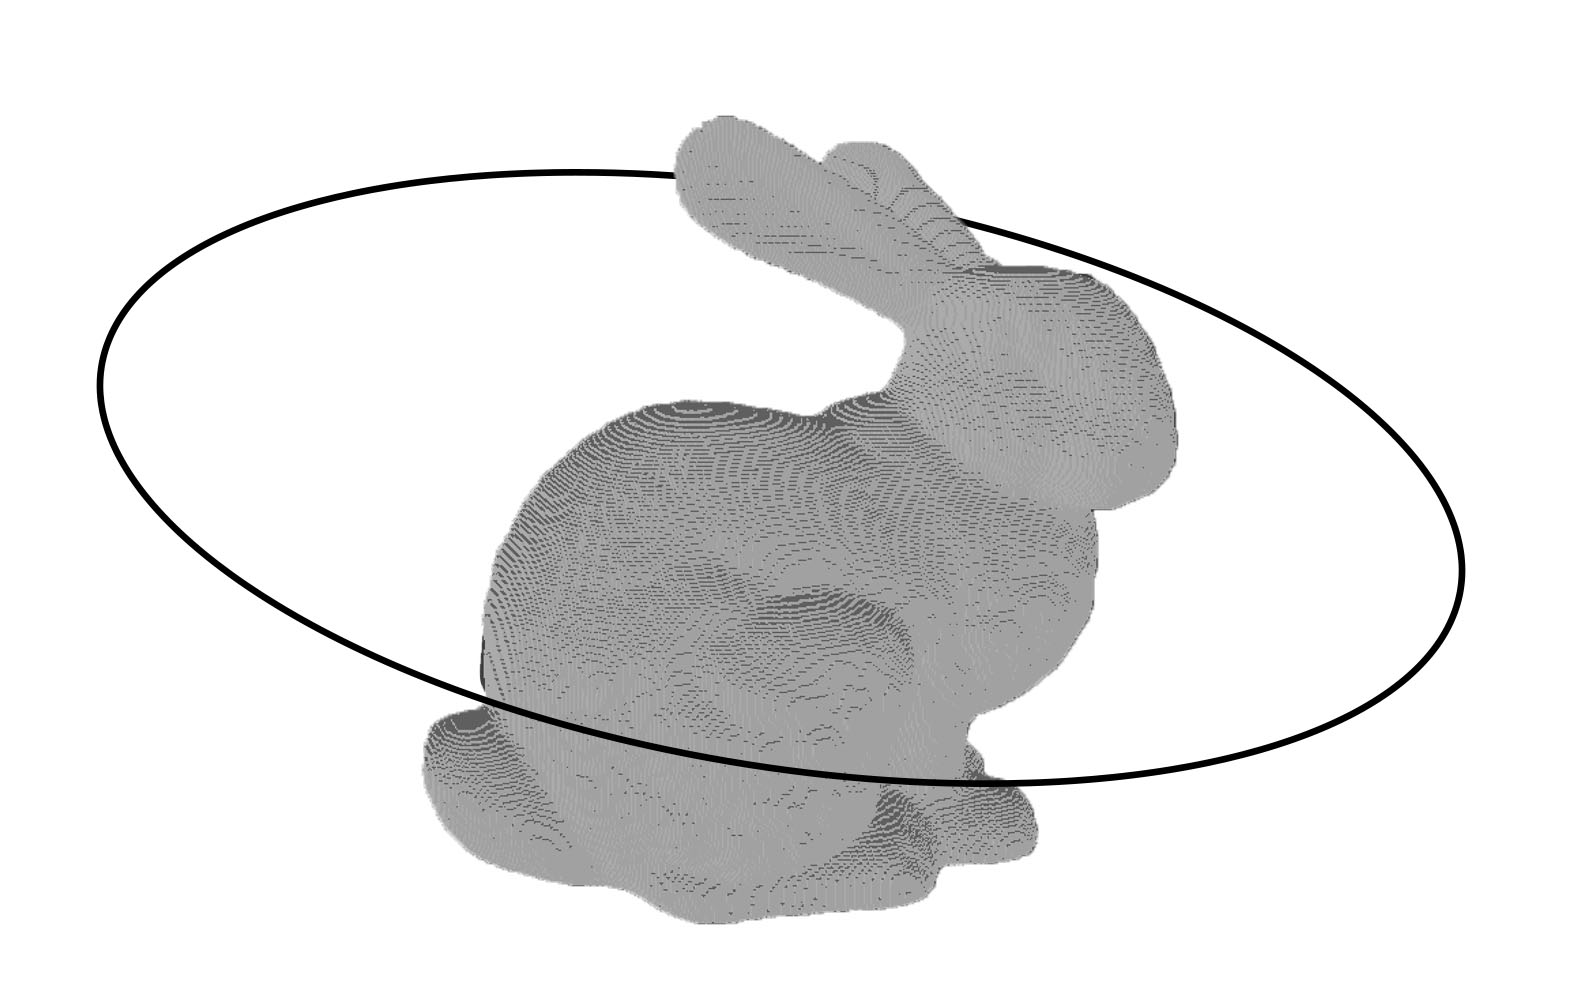
\includegraphics[width=200px]{images/graphics/test-anim-camera-path.jpg}
    \caption{During profiling, the camera is moved along an orbit around the voxel mesh, while being offset to compensate 
    for models, which behave differently when viewed from an angle. The visualization is not to scale, the models 
    are always completely visible and not culled by view frustum culling.}
    \label{fig:test-anim-camera-path}
\end{figure}

\noindent
[@TODO: Consider replacing the last "algorithm" with the actual subelement of the algo (scene data / data dispatch / ...)] 
Another aspect to consider is the model data structure. The voxel models are volumetric representations and thus 
not hollow. This leaves a large portion of the computation to be irrelevant and allows for the occlusion culling to 
optimize the data flow. Different types of models were used to challenge the culling algorithm in different ways. 
In concept, the culling should be optimal on large, dense models with even faces. Consequently, models with 
slopes and holes were tested to see how best occluders can be computed for diverse geometry. Smaller models might 
also pose a challenge for the optimization, especially when the octree nodes cannot be filled completely. Also, 
different voxel resolutions were used to achieve different amounts of octree nodes in the scene. All these different 
aspects aim to show the strengths and weaknesses of the algorithm and how it can be optimally used in practice. \\

\noindent
The resolution of the voxelization process played a central role in the experimentation process.
For the experiment, the voxel scenes were constrained to be a power of two in length per axis, and a resolution 
of $\emph{256} \times \emph{256} \times \emph{256}$ was used for the performance profiling, resulting in a maximum 
of \emph{16.777.216} voxels. In practice, the maximum amount of voxels was limited by how the data was dispatched 
by the \ac{GPU}. In the implementation, the shader model used (HLSL Shader Model 6.6) was limited to a maximum 
amount of 65.536 threadgroups. That means that the threadgroup size and the amount of constructed octree nodes 
influenced the possible resolutions of the scenes. This limitation can be overcome by scheduling more than one draw 
call, but for this experiment, only one draw call was used. Consequently, the actual maximum amount of voxels in the 
scene was around 3-4 million voxels, which was considered enough for this experiment.


\subsection*{Timings} \label{subsec-timings}

The time spent for various computations is relevant for the selection of the best algorithm. This is a central 
tool to see how the implementation performs overall in the context of the framework used. Consequently, the 
timingss for all major pipeline steps were conidered, as well as the overall time spent on \ac{CPU} and \ac{GPU} 
computations. \\

\noindent 
The overall framerate of the application was artificially clamped to 30, 60, or 120 \emph{Hz} by \emph{Diligent Engine}, 
depending on the connected monitor, which occasionally resulted in an abrupt changes of frame times. This also means 
that the overall frame time was not reliably showing the \ac{CPU} workload. However, measuring only the internal render 
and update routines provided more reliable results. This is why the overall frame time isn't used for further analysis, 
but is listed in Appendix \ref{cpt-appendix}.


\subsection*{Visibility and Culling} \label{subsec-visibility-and-culling}

In order to evaluate the general functionality and effectiveness of the pipeline, the voxel model was analyzed 
with and without the occlusion culling applied. The amount of culled voxels was compared to the total amount of 
voxels, resulting in an overview of how much geometry could be culled for different scene setups. The same is 
valid for the amount of octree nodes. They could also be compared to the number of best occluders. The more best 
occluders present in a scene, the higher the probability to occlude other voxels or octree nodes. To evaluate 
how much can be optimized during the depth prepass, the number of best occluders was compared to the number 
of voxels representing the best occluders. \\

\noindent
Finally, the actual amount of processed triangles was considered in order to show the actual geometry processed 
by the \ac{GPU}. This data indicates how much work is being scheduled for the vertex transformations, the rasterizer, 
and the pixel shader. Ultimately, it decides over the amount of overdraw and should therefore be kept at a minimum.


\subsection*{Measuring Tools} \label{subsec-measuring-tools}

To measure timings and data precisely, a few external tools were used. All tools are part of the industry 
standard and were therefore assumed to be mostly reliable. Still, measuring performance usually comes with 
a minimal overhead, which means that the results most likely vary in precision. Also, some of the tools 
provided various ways of sampling the data. Some data was measured while the profiled application was 
running, and other data was acquired by replaying the command list of the \ac{GPU}. Consequently, all 
measurements referring to one aspect of the application were compared against measurements using the same 
tool and configuration, if not explicitly specified otherwise. \\

\noindent
For the collection of data output, \emph{RenderDoc} \cite{RenderDoc} was used. It is a free, MIT-licensed 
rendering debugger, widely used in the industry. For \emph{NVIDIA}-specific \ac{GPU} profiling, \emph{NVIDIA NSight} 
\cite{NSight} was used, which is another industry standard profiling and debugging tool. It is only available for 
inspection of \emph{NVIDIA} graphics card computations but provided valuable insights into the rendering pipeline 
and hardware usage. The last tool used is \emph{Microsoft's PIX} \cite{PIX}, which is another performance debugging 
and profiling tool for \emph{Windows} platforms using \emph{Microsoft's DirectX} \ac{API}. \\

\noindent
The culling result measurements were directly sampled from the \emph{task shader} over the course of the testing 
animation, using \emph{RenderDoc} and emph{PIX}. They were generally independent from the hardware and rather 
depended on the camera position and viewing angle as well as on model resolution. Also, the screen resolution 
affected the amount of mips generated for the \ac{HiZ} pyramid, so it was fixed to $1280 \times 900$ pixels. 
All of the aspects above were standardized for each model over all test runs.


\subsection*{Experimental Environment} \label{subsec-experimental-environment}

[@TODO: Rethink section title]
For the experiment, different hardware setups were used to compare the runtime performance in different environments.
Some more modern hardware was used to profile the best-case computations, and older hardware was used for the results 
to different versions of hardware features and capabilities.

\begin{table}[h]          % System setup table
    \begin{tabular}{|lll|}
        \hline
        \multicolumn{3}{|c|}{\textbf{Test setups}}                                                                              \\ \hline
        \multicolumn{1}{|l|}{}                     & \multicolumn{1}{l|}{\textbf{Setup 1}}          & \textbf{Setup 2}          \\ \hline
        \multicolumn{1}{|l|}{\textbf{System Type}} & \multicolumn{1}{l|}{Desktop}                   & Laptop                    \\
        \multicolumn{1}{|l|}{\textbf{CPU}}         & \multicolumn{1}{l|}{AMD Ryzen 9 9950X}         & Intel Ultra 7 155H        \\
        \multicolumn{1}{|l|}{\textbf{Cores}}       & \multicolumn{1}{l|}{16 (32)}                   & 16 (22)                   \\
        \multicolumn{1}{|l|}{\textbf{RAM}}         & \multicolumn{1}{l|}{96 GB}                     & 16 GB                     \\
        \multicolumn{1}{|l|}{\textbf{GPU}}         & \multicolumn{1}{l|}{NVIDIA GeForce RTX 4090}   & Intel Arc Graphics        \\
        \multicolumn{1}{|l|}{\textbf{VRAM}}        & \multicolumn{1}{l|}{24 GB}                     & 128 MB (+ 8972 MB shared) \\
        \multicolumn{1}{|l|}{\textbf{OS}}          & \multicolumn{1}{l|}{Windows 10}                & Windows 11                \\
        \multicolumn{1}{|l|}{\textbf{Model}}       & \multicolumn{1}{l|}{-}                         & ASUS Zenbook 14 (2024)    \\ \hline
    \end{tabular}
    \caption{The experimental setups used to profile the applications performance.}
    \label{tbl:hardware-setup}
\end{table}

\noindent
Note that the use of the Mesh Shading pipeline requires graphics cards that support the pipeline in the first place. 
For \emph{NVIDIA} \ac{GPU}s, this is the \emph{Turing} lineup (\emph{NVIDIA RTX 20 series}), and for \emph{AMD} cards, 
this would be the \emph{RDNA 2} lineup (\emph{AMD RX 6000 series}). \emph{Intel} \ac{GPU}s support the feature as 
well, starting from their first installment in the dedicated desktop \ac{GPU} series \emph{Intel Arc}. The specs of 
the test setups are listed in table \ref{tbl:hardware-setup}. \\


\subsection*{Models} \label{subsec-models}

\begin{figure}[h]
  \centering
  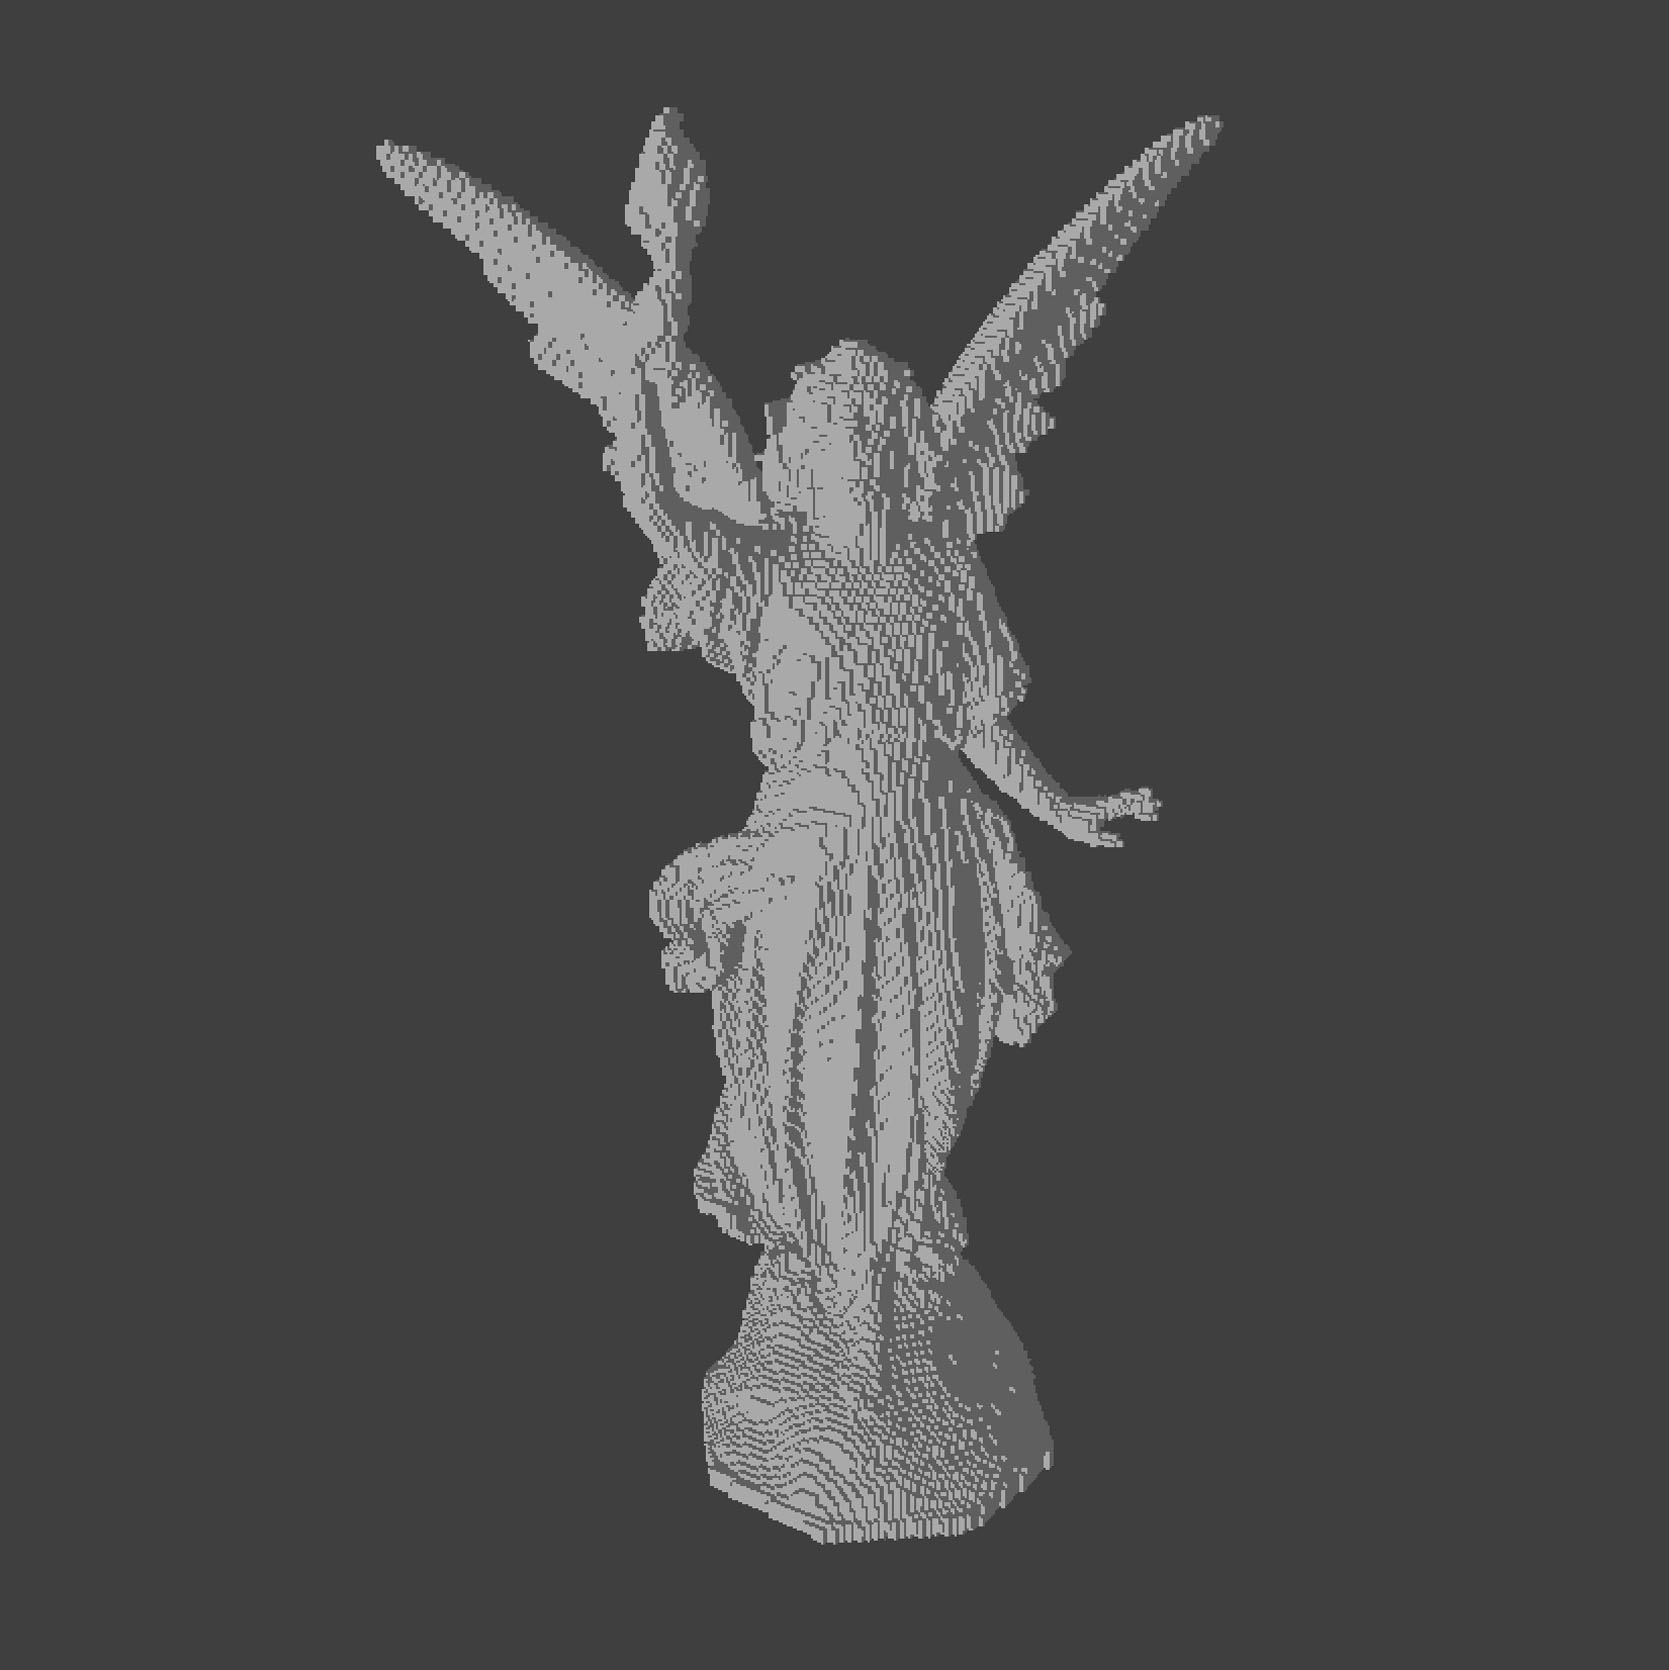
\includegraphics[width=80px]{images/graphics/model-lucy.jpg}
  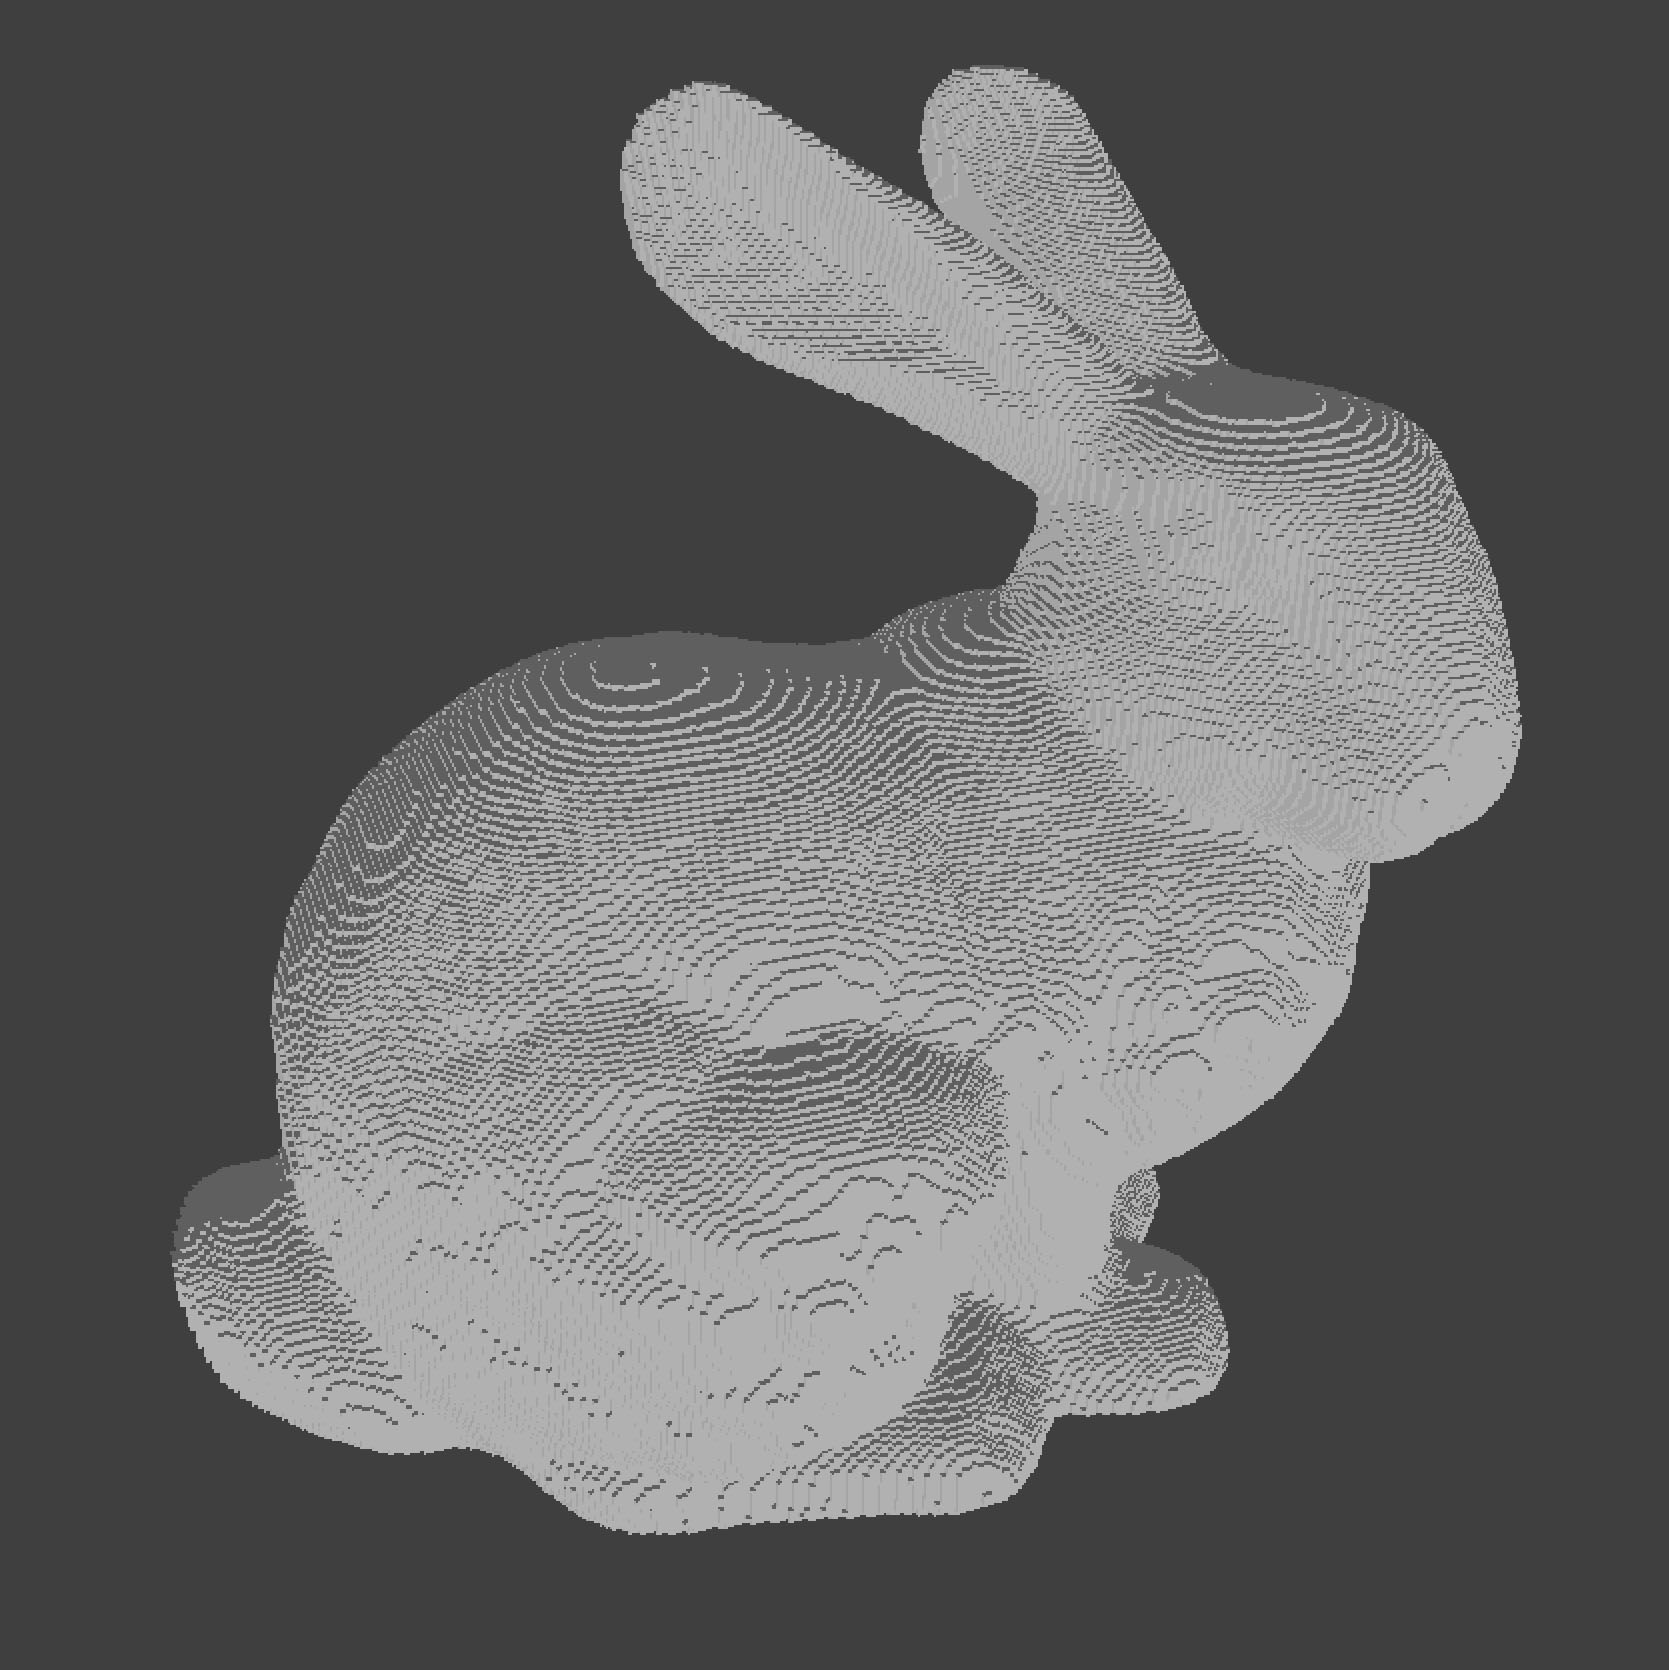
\includegraphics[width=80px]{images/graphics/model-bunny.jpg}
  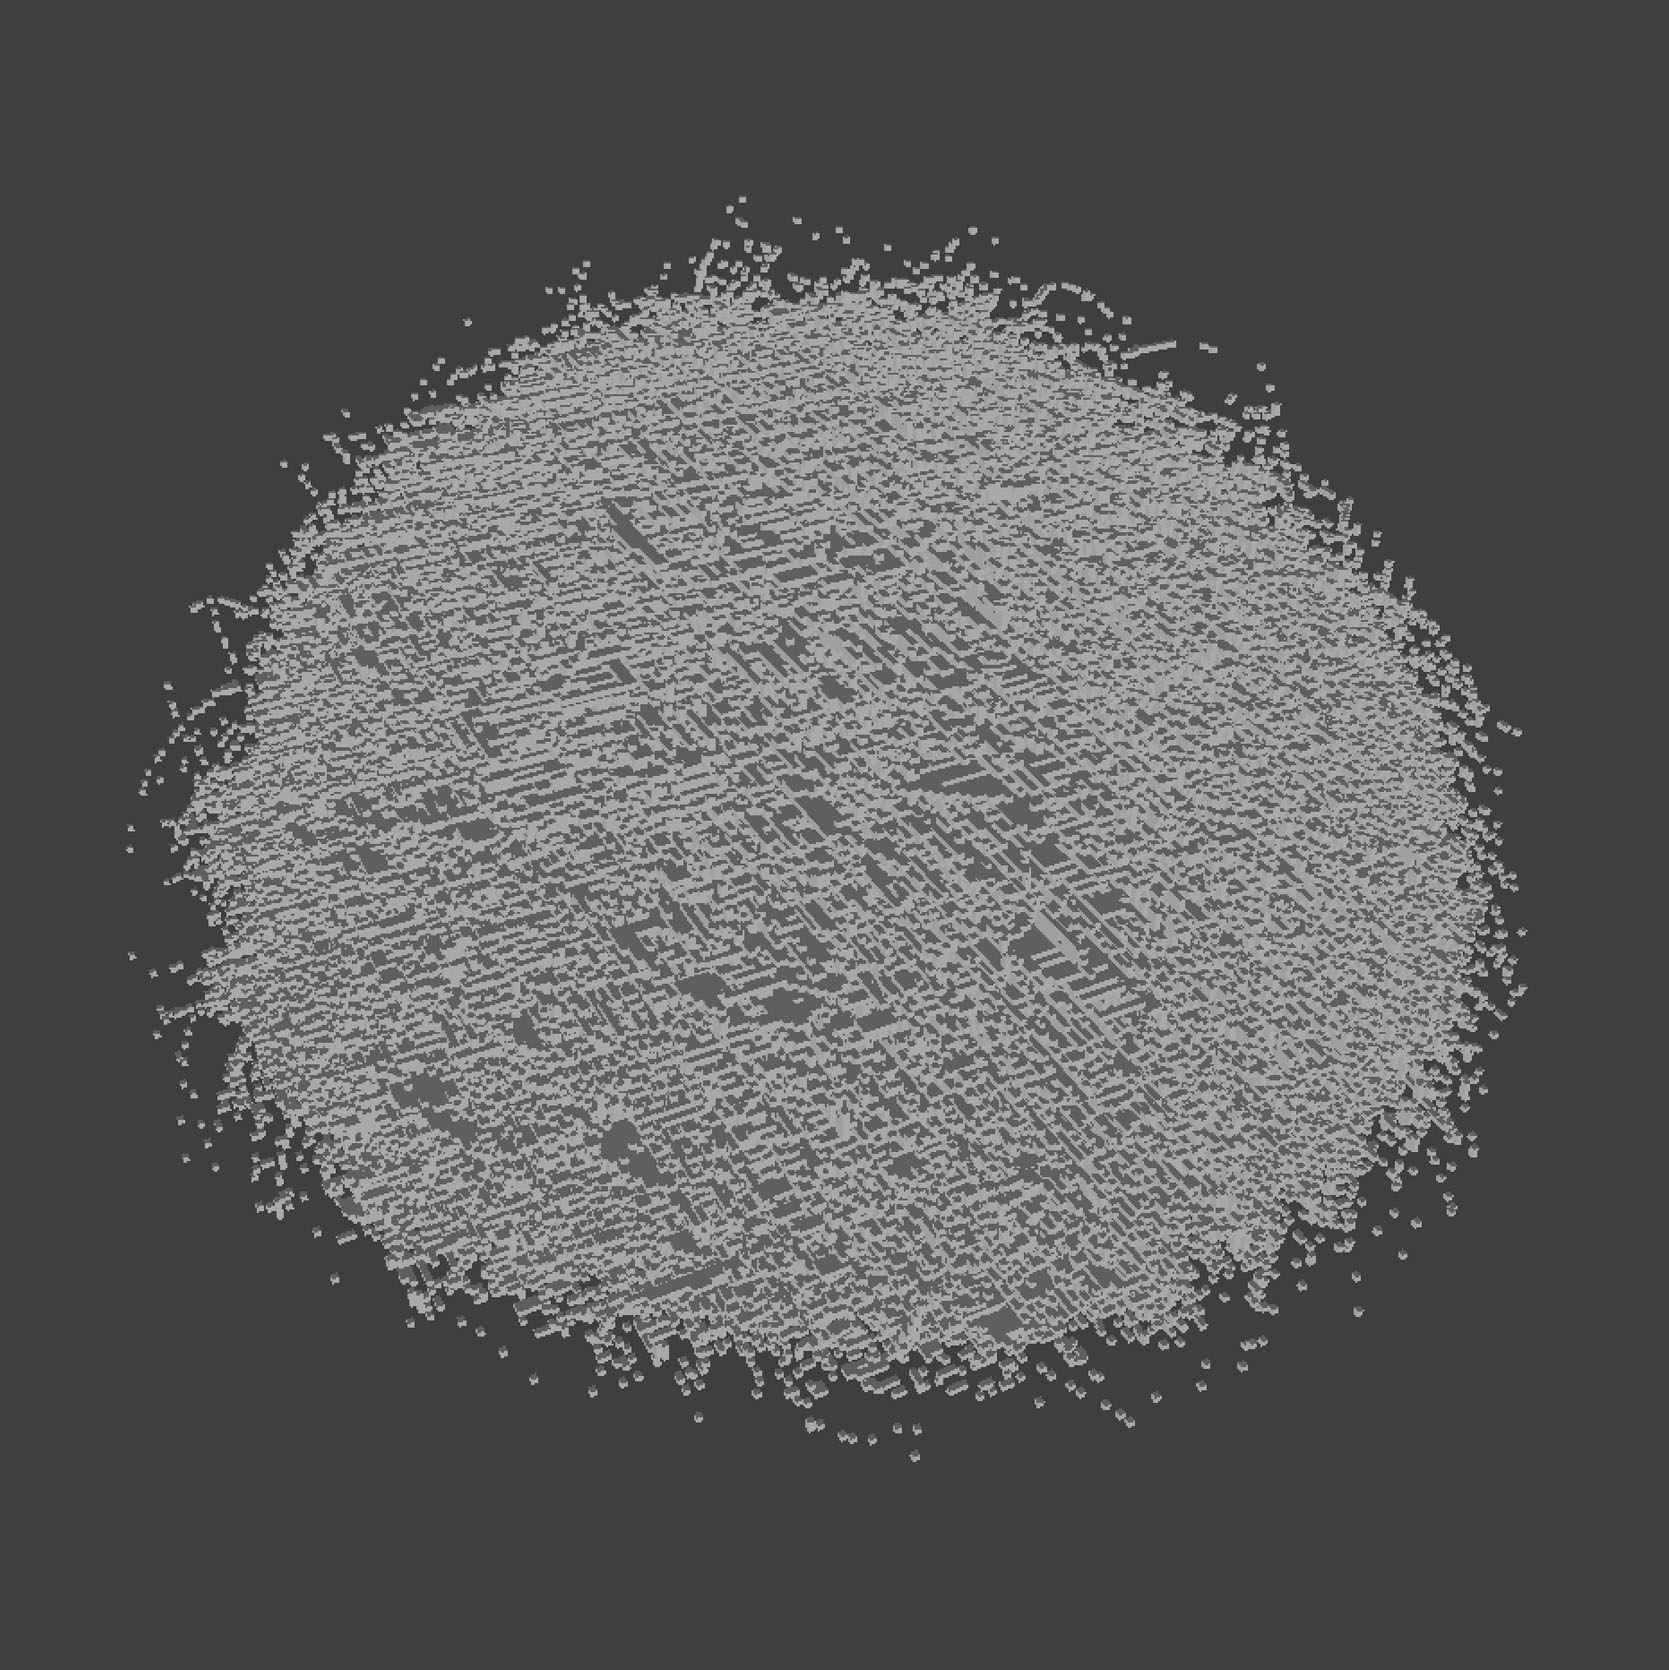
\includegraphics[width=80px]{images/graphics/model-hairball.jpg}
  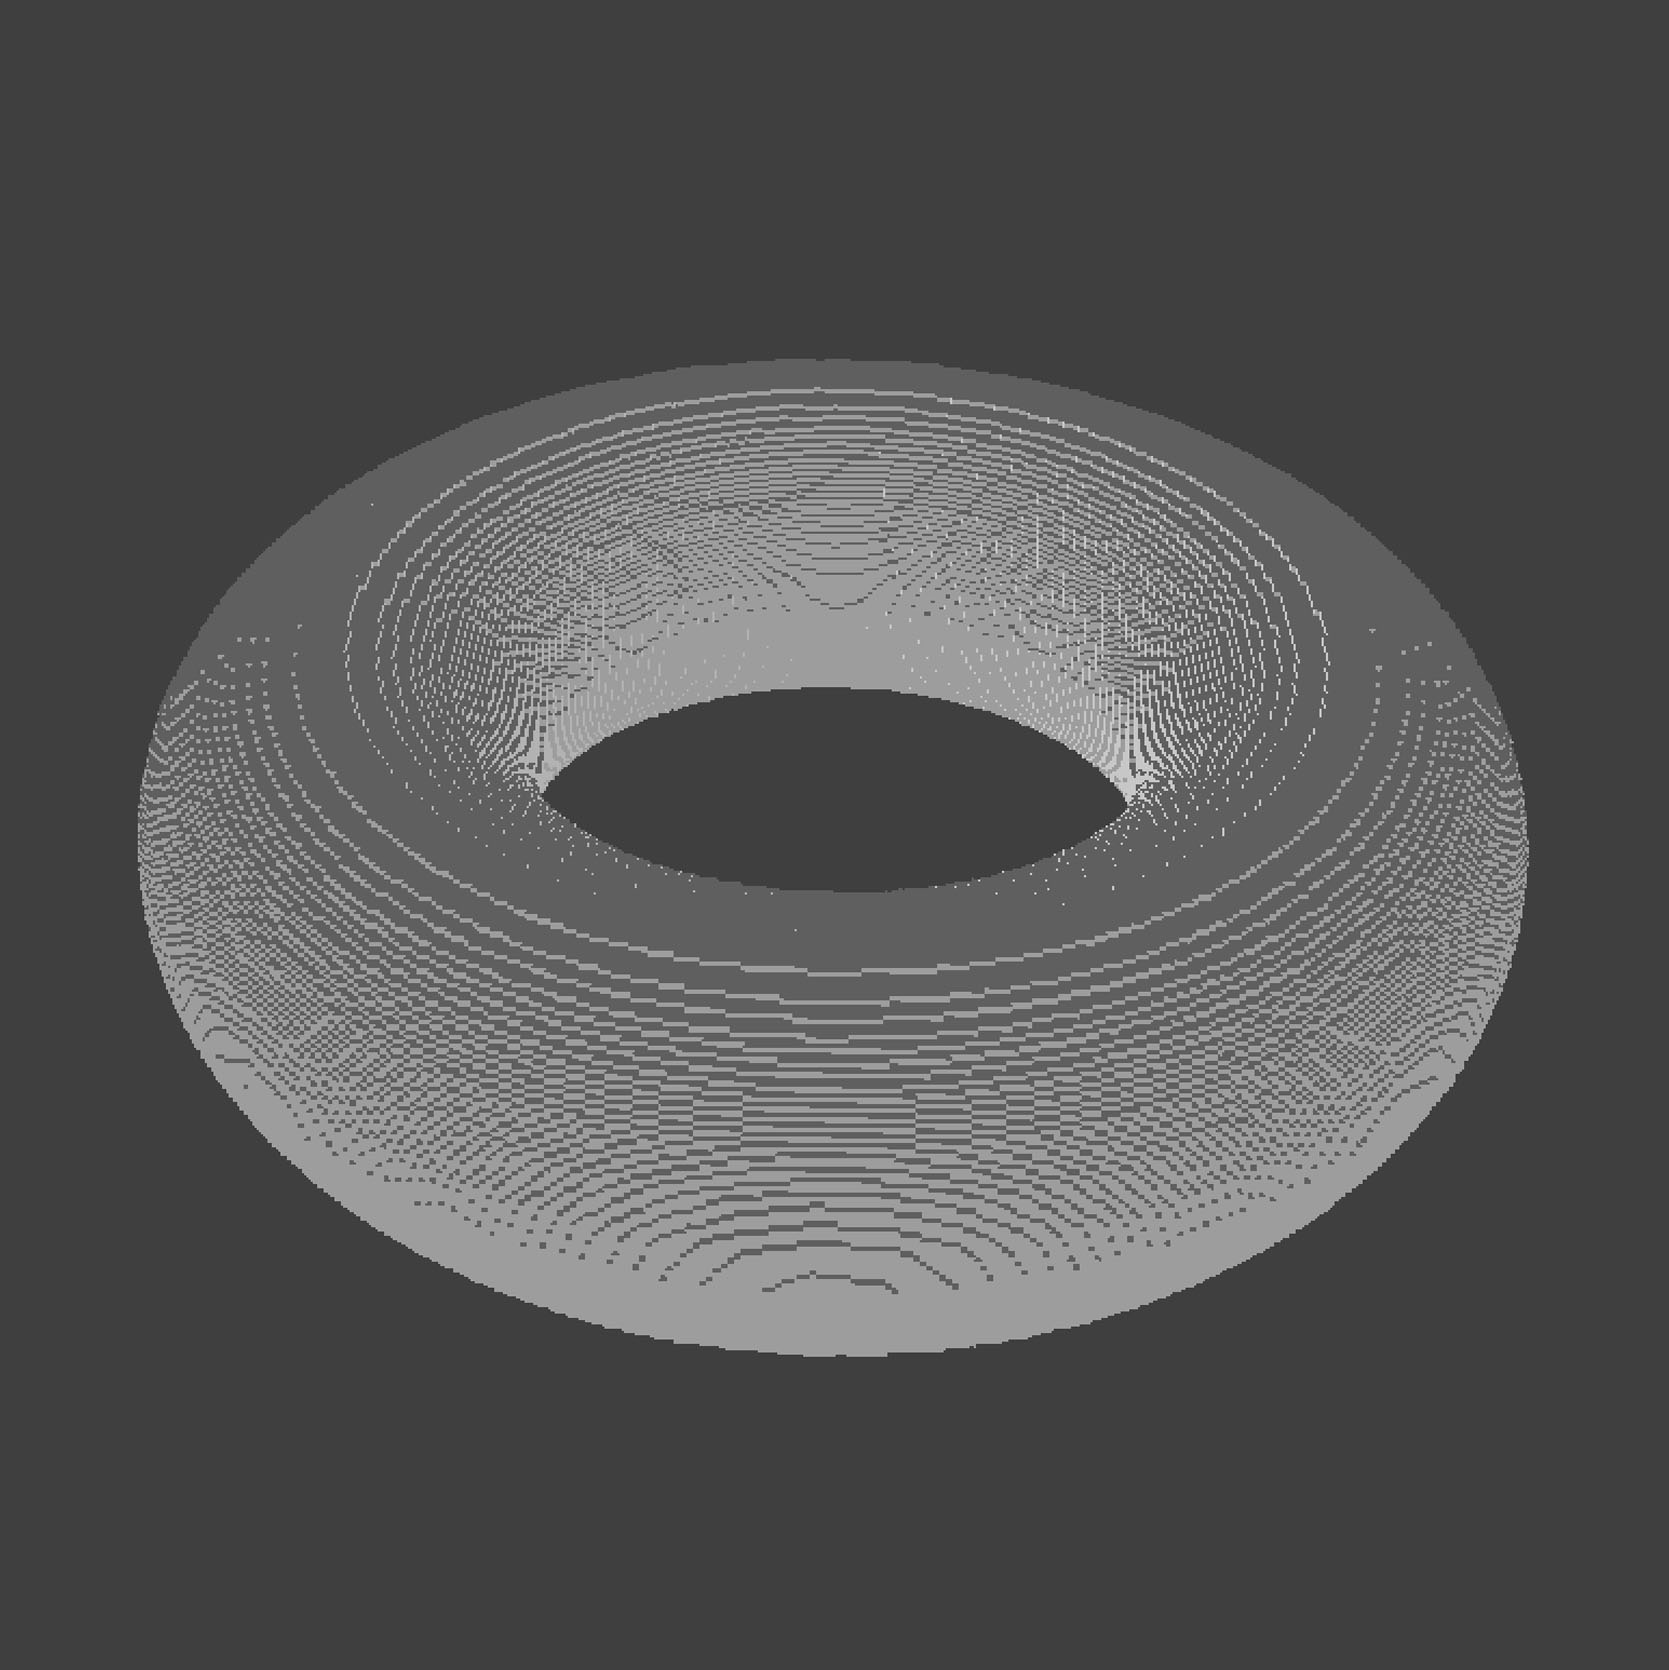
\includegraphics[width=80px]{images/graphics/model-torus.jpg}
  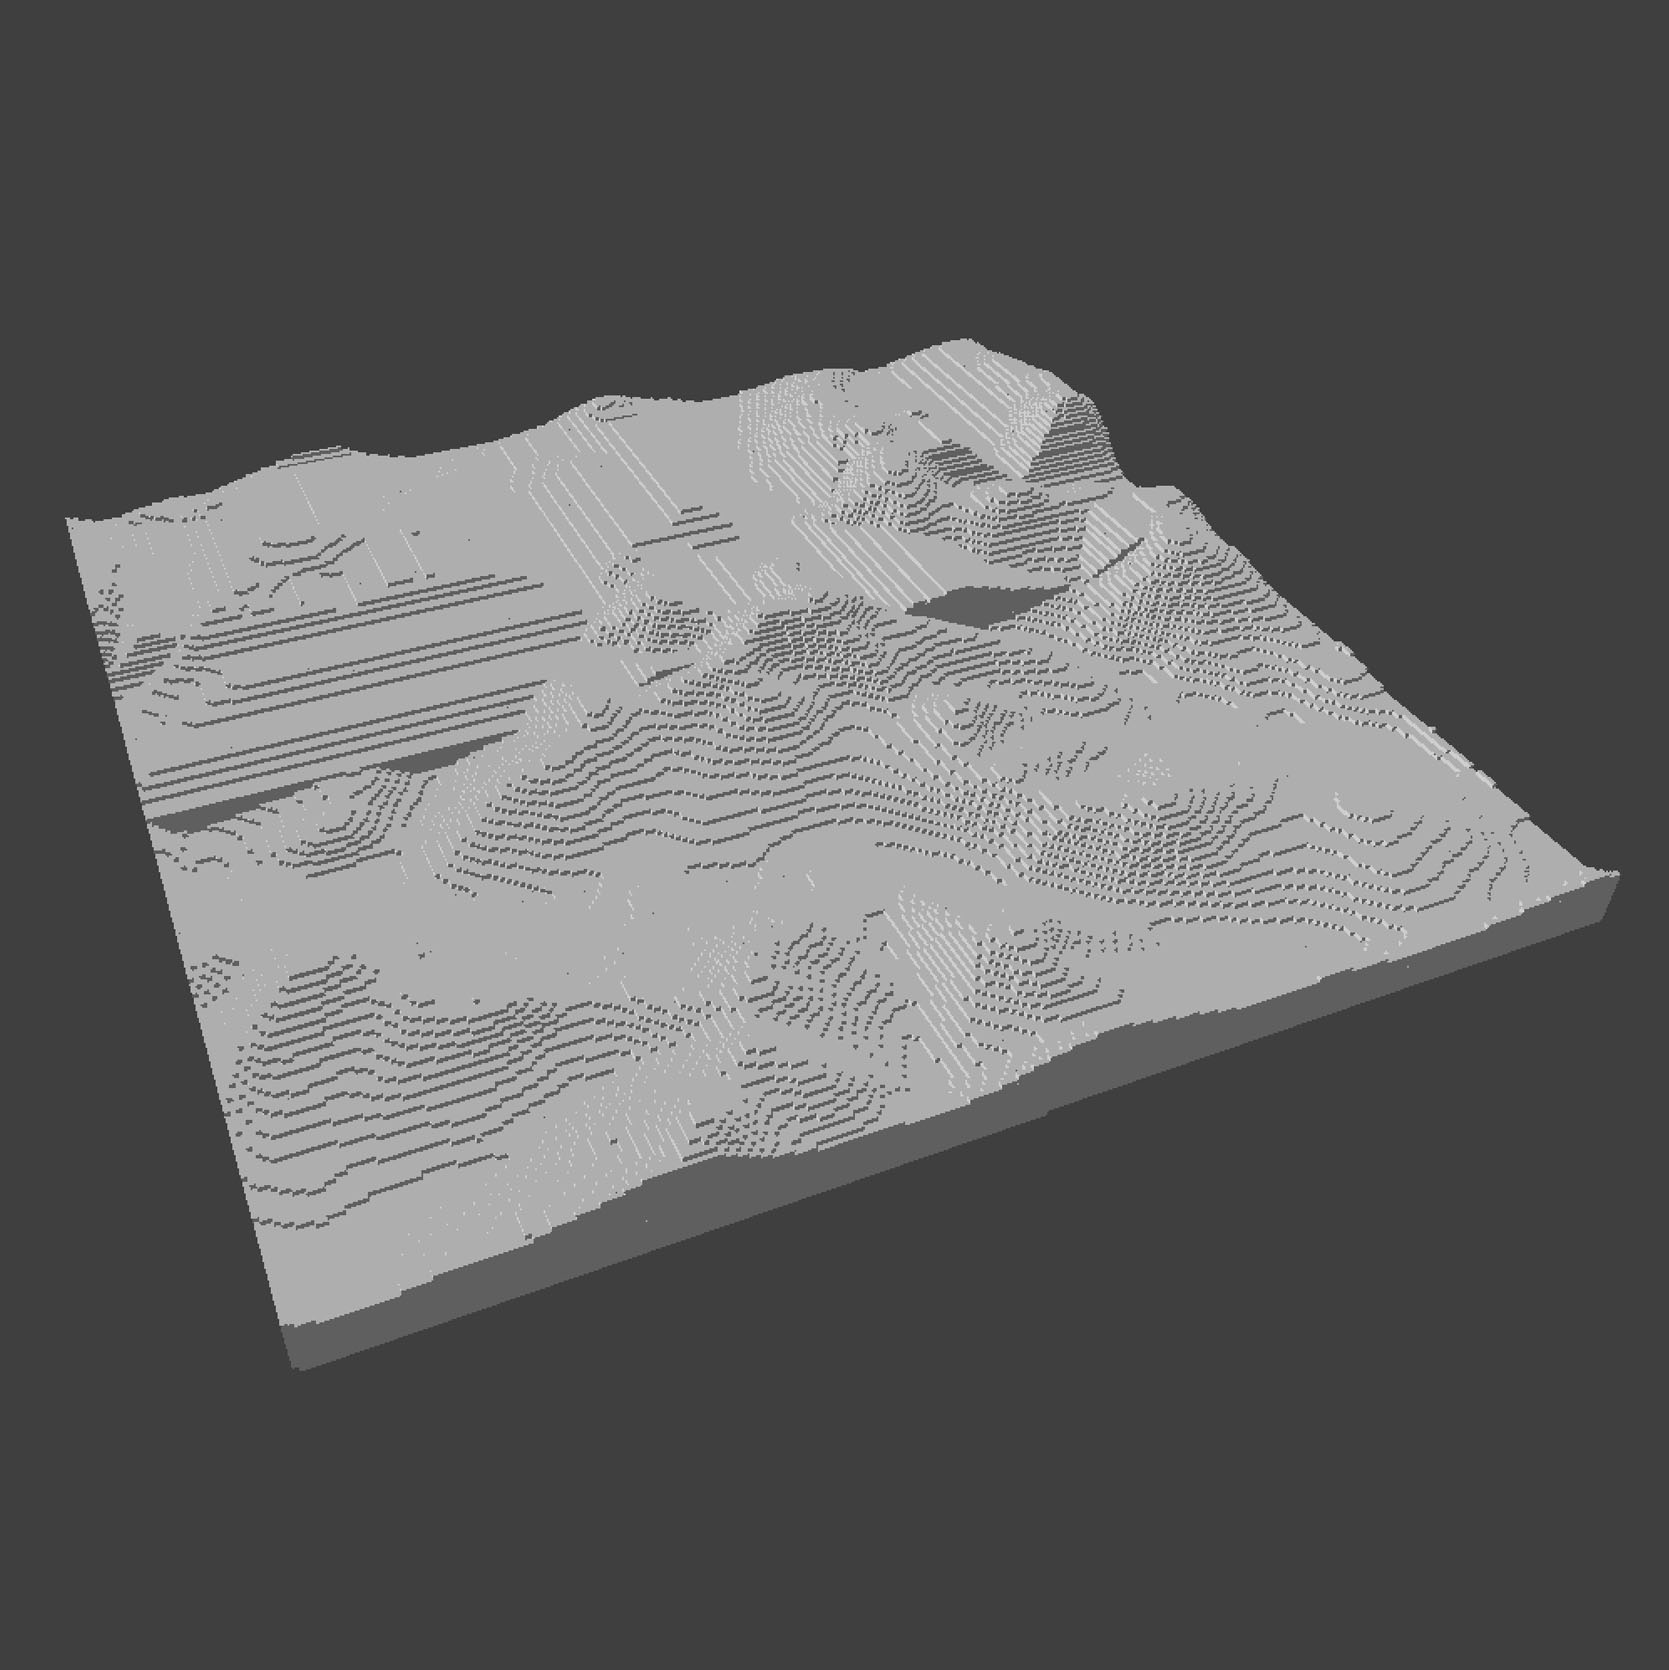
\includegraphics[width=80px]{images/graphics/model-terrain.jpg}
  \caption{The models used for the experiment.}
  \label{fig:experiment-models}
\end{figure}

\noindent
The models that were used in the tests are \emph{Lucy} (Stanford 3D Scanning Repository), the 
\emph{Stanford Bunny} (Stanford 3D Scanning Repository), the \emph{Hairball}, a \emph{Torus}, 
and a \emph{Terrain} scene. All of these models provide different characteristics, which tested 
the pipeline in a variety of ways. They were voxelized to a scene size of $256^3$ and occupy 
different amounts of space in the scene.

[@TODO: Write a bit more here.]



[@TODO: Add memory footprint to data throughput]


\section{Experimental Results}

In this section, the experimental results are presented and discussed for each model tested.
For each model, the culling results include data that isn't dependent on specific hardware. 
After that, the profiling measurements are discussed, which relate to the hardware setup presented 
in \ref{subsec-experimental-environment}. The data analysis is structured similarly for all models,
comparing the \ac{PONOC} configuration to the \ac{PMOC} configuration. Finally, an overview 
is presented that summarizes all the relevant data in a compact visualization.

[@TODO: Update (Prepass) Labels (like Generate HiZ Pyramid instead of GenMipChain)]

\subsection*{Best Occluder Selection}

To evaluate the best occluder selection, all models were tested in terms of the octree's 
query for the best occluders. 

\begin{table}[htbp]
  \begin{center}
    \begin{tabular}{|c|c|c|c|}
      \hline
      \textbf{}&\multicolumn{3}{|c|}{\textbf{Best Occluder Selection - $256^3$}} \\
      \cline{2-4} 
      \textbf{Scene} & \textbf{\textit{Voxel Count}}& \textbf{\textit{Best Occluder Count}}& \textbf{\textit{Time (ms)}} \\
      \hline
      Lucy        & 331,254   & 1600 & 0.317 \\
      Bunny       & 3,379,738 & 8256 & 3.752 \\
      Torus       & 2,311,006 & 7168 & 2.681 \\
      Terrain     & 953,362   & 6976 & 1.267 \\
      Hairball    & 1,652,435 & 5056 & 2.377 \\
      \hline
    \end{tabular}
    \caption{Measurements of best occluder query.}
  \label{tab:best-occluder-query}
  \end{center}
\end{table}


\subsection*{Stanford Lucy}

The \emph{Lucy} model is tall and slim, which means that its volume is distributed more over one axis 
than over the other two axis. This is assumed to provide interesting insights into how such an object 
self-occludes the voxels when viewed from different perspectives. It also has a few narrow parts where 
no best occluders are expected.

\subsubsection*{Culling Results} \label{subsubsec-culling-results-lucy}

% --------------------------------------- LUCY 256 ---------------------------------------

\begin{figure}[!htb]              % Lucy 256 Culling Res
    \begin{center}
      \begin{tikzpicture}
        \begin{axis}[
            width=\linewidth, % Scale the plot to \linewidth
            height=100px,
            xlabel={Frames},
            ylabel={VComputed Voxels},
            grid,
            xmin=0,
            xmax=2392,
            ymin=60000,
            ymax=160000,
            legend style={at={(0.5,1.7)}, anchor=north, legend columns=2},
          ]
          \addplot[blue, no marks, solid] table[col sep=comma, x=frame, y=visible_voxels]{./plotdata/lucy_256_voxels.csv};
          \addplot[blue, dotted, no marks, domain=0:2393, samples=50] {140842};
          \addplot[red, no marks, solid] table[col sep=comma, x=frame, y=visible_voxels]{./plotdata/lucy_256_voxels_pmoc.csv};
          \addplot[red, dotted, no marks, domain=0:2393, samples=50] {84082};
          \legend{Per-Octree Occlsion Culling, Per-Meshlet Occlusion Culling}
        \end{axis}
      \end{tikzpicture}
      \begin{tikzpicture}
        \begin{axis}[
            width=\linewidth, % Scale the plot to \linewidth
            height=100px,
            xlabel={Frames},
            ylabel={Computed Nodes},
            grid,
            xmin=0,
            xmax=2392,
            ymin=1800,
            ymax=4000,
            legend style={at={(0.5,1.7)}, anchor=north, legend columns=2},
          ]
          \addplot[blue, no marks, solid] table[col sep=comma, x=frame, x expr=\thisrow{frame} * 2392 / 2392, y=visible_nodes]{./plotdata/lucy_256_nodes.csv};
          \addplot[blue, dotted, no marks, domain=0:2393, samples=50] {3460};
          \addplot[red, no marks, solid] table[col sep=comma, x=frame, x expr=\thisrow{frame} * 2392 / 2395, y=visible_nodes]{./plotdata/lucy_256_nodes_pmoc.csv};
          \addplot[red, dotted, no marks, domain=0:2393, samples=50] {2483};
          \legend{Per-Octree Occlsion Culling, Per-Meshlet Occlusion Culling}
        \end{axis}
      \end{tikzpicture}
      \caption{First: The amount of visible voxels over the course of the test animation. 
      Second: The amount of visible octree nodes over the course of the test animation.}
      \label{plt:lucy-256-culling-culling-results}
    \end{center}
  \end{figure}

% ----------------------------------------------------------------------------------------

\noindent
Figure \ref{plt:lucy-256-culling-culling-results} shows the amount of visible voxels and visible octree 
nodes for both the \ac{PONOC} (upper graph) and the \ac{PMOC} 
(lower graph) configuration. \\

\noindent [@TODO: Fix plot color references]
The average amount of visible voxels was \emph{140,842} for \ac{PONOC}, which is marked 
as the blue dotted line, and \emph{84,082} for \ac{PMOC}, marked in red. The average 
amount of visible octree nodes was \emph{3,460} for \ac{PONOC}, which is marked as the 
blue dotted line, and \emph{2,483} for \ac{PMOC}, which is marked as the red dotted 
line. \\

\noindent
[@TODO: Consider moving explanations and further analysis to discussion part.]
It is obvious that the per-meshlet culling significantly reduced the amount of dispatched voxels and octree nodes, 
which lead to less load for the rasterizer and the pixel shader. The amount of octree nodes decreased when using 
per-meshlet culling because octree nodes could be culled, even when their corners were visible by the camera. 
For instance, when considering a node that holds just 5 voxels, which are all overlapped by a part of the model, 
this octree node will be inherently culled when using per-meshlet culling. Contrary, when using per-octree culling, 
the culling is dependent on the visibility of any of the octree node's corners, which can result in a node being not 
culled, even though all voxels within that node remain occluded. \\

\noindent 
Both curves indicate how the model fits the overall culling algorithm. For instance, the \emph{Stanford Lucy} 
model has a relatively even curve over time. Of course, this is a dynamic measure and highly depends on the 
angle of the camera. Still, the compact, tall model provides a good amount of best occluders to occlude a 
relatively even number of voxels when viewed from the side. \\

\noindent
Considering the average amount of visible voxels, the per-octree algorithm was able to cull $57.5\%$ of all 
voxels. On average, the per-meshlet culling even managed to omit $74.6\%$ of all voxels. 

\subsubsection*{CPU Performance Results} \label{subsubsec-cpu-performance-results-lucy}

\begin{figure}[!htb]              % Lucy renderTimes
  \begin{center}
    \begin{tikzpicture}
      \begin{axis}[
          width=\linewidth,
          height=100px,
          xlabel={Frames},
          ylabel={Update Time (s)},
          grid,
          xmin=0,
          xmax=2392,
          ymin=0,
          ymax=0.00005,
          legend style={at={(0.5,1.7)}, anchor=north, legend columns=2},
        ]
        \addplot[brown!60, no marks, solid] table[col sep=comma, x=frame, x expr=\thisrow{frame} * 2392 / 1648, y=time]{./plotdata/cpu/lucy_256_updateTime_nocull.csv};
        \addplot[blue, no marks, solid] table[col sep=comma, x=frame, x expr=\thisrow{frame} * 2392 / 1863, y=time]{./plotdata/cpu/lucy_256_updateTime_pooc.csv};
        \addplot[red, no marks, solid] table[col sep=comma, x=frame, x expr=\thisrow{frame} * 2392 / 1867, y=time]{./plotdata/cpu/lucy_256_updateTime.csv};
        \legend{No Occlusion Culling, Per-Octree Occlsion Culling, Per-Meshlet Occlusion Culling}
      \end{axis}
    \end{tikzpicture}
    \begin{tikzpicture}
      \begin{axis}[
          width=\linewidth,
          height=100px,
          xlabel={Frames},
          ylabel={Render Time (s)},
          grid,
          xmin=0,
          xmax=2392,
          ymin=0,
          ymax=0.00025,
          legend style={at={(0.5,1.7)}, anchor=north, legend columns=2},
        ]
        \addplot[brown!60, no marks, solid] table[col sep=comma, x=frame, x expr=\thisrow{frame} * 2392 / 1648, y=time]{./plotdata/cpu/lucy_256_renderTime_nocull.csv};
        \addplot[blue, no marks, solid] table[col sep=comma, x=frame, x expr=\thisrow{frame} * 2392 / 1863, y=time]{./plotdata/cpu/lucy_256_renderTime_pooc.csv};
        \addplot[red, no marks, solid] table[col sep=comma, x=frame, x expr=\thisrow{frame} * 2392 / 1867, y=time]{./plotdata/cpu/lucy_256_renderTime.csv};
        \legend{No Occlusion Culling, Per-Octree Occlsion Culling, Per-Meshlet Occlusion Culling}
      \end{axis}
    \end{tikzpicture}
    \caption{Overview of the render times over the course of the test animation. The first graph shows the time 
    each frame took to execute the \emph{Update()} function on the \ac{CPU}. The second graph shows the time each 
    frame took to execute the \emph{Render()} function on the \ac{CPU}. This includes the completion of the 
    \ac{GPU} computations.}
    \label{plt:lucy-256-culling-cpu-time}
  \end{center}
\end{figure}

\noindent
Figure \ref{plt:lucy-256-culling-cpu-time} shows the \ac{CPU} computations over the course of the test animation.
The first graphs shows the computation of the \ac{CPU} \emph{Update()} function, which includes updating the camera's 
view and projection matrices. This function was expected to be static in runtime, regardless of the culling configuration. 
The graph shows that this is generally correct, as both are not significantly diverging.\\

\noindent
The second graph shows the isolated computation time of the \ac{CPU} \emph{Render()} function. It is a good indicator of 
how the computation time changed, and it includes the \ac{GPU} work that was called during the function, like 
\emph{DispatchMesh()} during the depth prepass and the final draw call. \\

\noindent
In general, the time spent on the most significant \ac{CPU} computations was pretty much static for this specific 
model. This result is as expected, as most of the work was executed on the \ac{GPU}, including the creation of the 
voxel meshes. After all, this approach is \ac{GPU}-driven at its core, so the bandwidth is small and the culling 
completely happens on the \ac{GPU} end of the pipeline.

\subsubsection*{GPU Performance Results} \label{subsubsec-gpu-performance-results-lucy}

On the \ac{GPU}, the \ac{PMOC} turned out to be faster in computation. As the occlusion 
culling algorithm intended, the time spent drawing the meshes could be reduced by $30\%$ on average for this 
particular model.

\begin{figure}[!htb]      % Lucy GPU Results
  \centering
  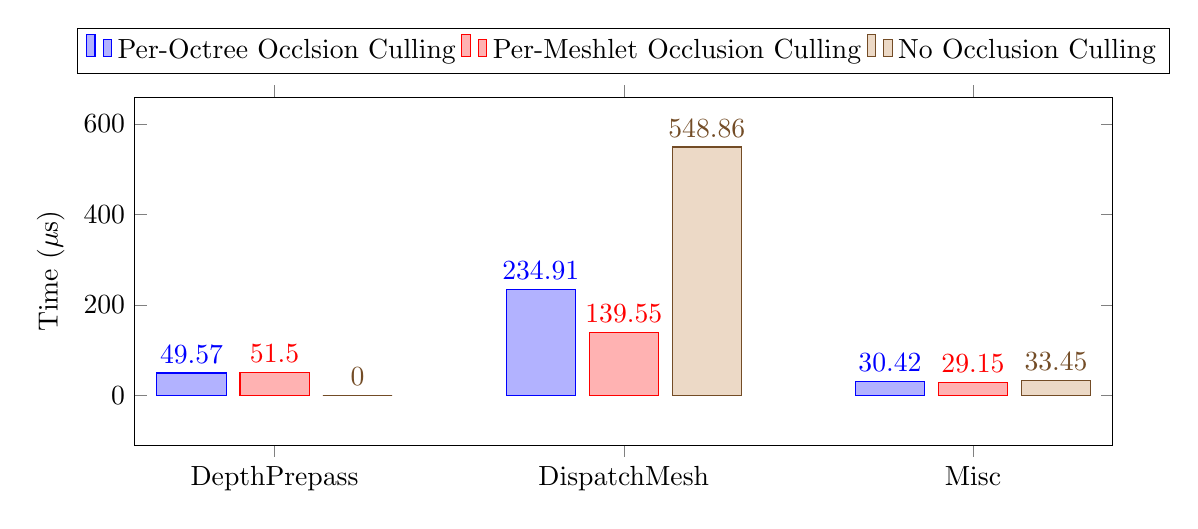
\begin{tikzpicture}
    \begin{axis}[
        height=6cm,
        width=14cm,
        x tick label style={/pgf/number format/1000 sep=},
        ylabel={Time ($\mu$s)},
        legend style={at={(0.5,1.2)}, anchor=north, legend columns=-1},
        symbolic x coords={DepthPrepass, DispatchMesh, Misc},
        xtick=data,
        ybar=0.4,
        bar width=25pt,
        ymin=0,
        nodes near coords,
        enlargelimits=0.2,
    ]
    \addplot+[bar shift=-30pt] coordinates {(DepthPrepass,49.57) (DispatchMesh,234.91) (Misc,30.42)};
    \addplot+[bar shift=0pt] coordinates {(DepthPrepass,51.50) (DispatchMesh,139.55) (Misc,29.1476)};
    \addplot+[bar shift=30pt] coordinates {(DepthPrepass,0) (DispatchMesh,548.86) (Misc,33.45)};
    \legend{Per-Octree Occlsion Culling, Per-Meshlet Occlusion Culling, No Occlusion Culling}
    \end{axis}
  \end{tikzpicture}

  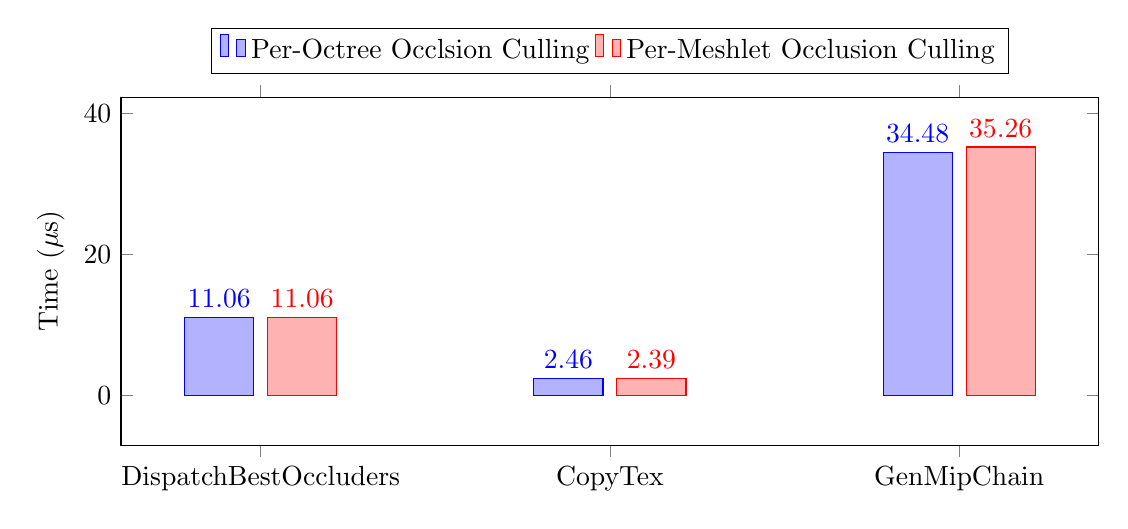
\begin{tikzpicture}
    \begin{axis}[
        height=6cm,
        width=14cm,
        x tick label style={/pgf/number format/1000 sep=},
        ylabel={Time ($\mu$s)},
        legend style={at={(0.5,1.2)}, anchor=north, legend columns=-1},
        symbolic x coords={DispatchBestOccluders, CopyTex, GenMipChain},
        xtick=data,
        ybar=0.4,
        bar width=25pt,
        ymin=0,
        nodes near coords,
        enlargelimits=0.2,
    ]
    \addplot+[bar shift=-15pt] coordinates {(DispatchBestOccluders,11.06) (CopyTex,2.46) (GenMipChain,34.48)};
    \addplot+[bar shift=15pt] coordinates {(DispatchBestOccluders,11.06) (CopyTex,2.39) (GenMipChain,35.26)};
    \legend{Per-Octree Occlsion Culling, Per-Meshlet Occlusion Culling}
    \end{axis}
  \end{tikzpicture}

  \caption{First: The complete time measured on the \ac{GPU}. The \emph{Depth Prepass} is the extra overhead 
  introduced by the \ac{HZB}. The \emph{Dispatch Mesh} is the drawing of the meshes, including the occlusion 
  culling. \emph{Miscellaneous} includes a small amount of \emph{Barriers} used for synchronisation and the 
  rendering of some debug \ac{UI}. It is considered to be more or less static in computation time and is not 
  part of the actual algorithm measured in this experiment. Second: The time measured in the \emph{Depth Prepass}. 
  The \emph{Dispatch Best Occluders} is the drawing to the depth buffer. The \emph{Copy Depth Buffer} computation 
  copies the depth buffers content into the final \ac{HiZ} resource. Finally, \emph{Generate HiZ Pyramid} shows 
  the \ac{HiZ} creation, which is done sequentially.}
\end{figure}

\noindent
The comparison of the depth prepass shows a small difference in computation time. The per-octree node configuration 
terminated faster by $1.93$ microseconds on average. In this case, the difference was created by small deviations in 
copying the depth buffer and computing the mip maps. 

\subsubsection*{Overdraw}

\begin{figure}[!htb]
  \centering
  
\includegraphics[height=100px]{images/graphics/overdraw-lucy1-nocull.png}
  
\includegraphics[height=100px]{images/graphics/overdraw-lucy1-pooc.png}
  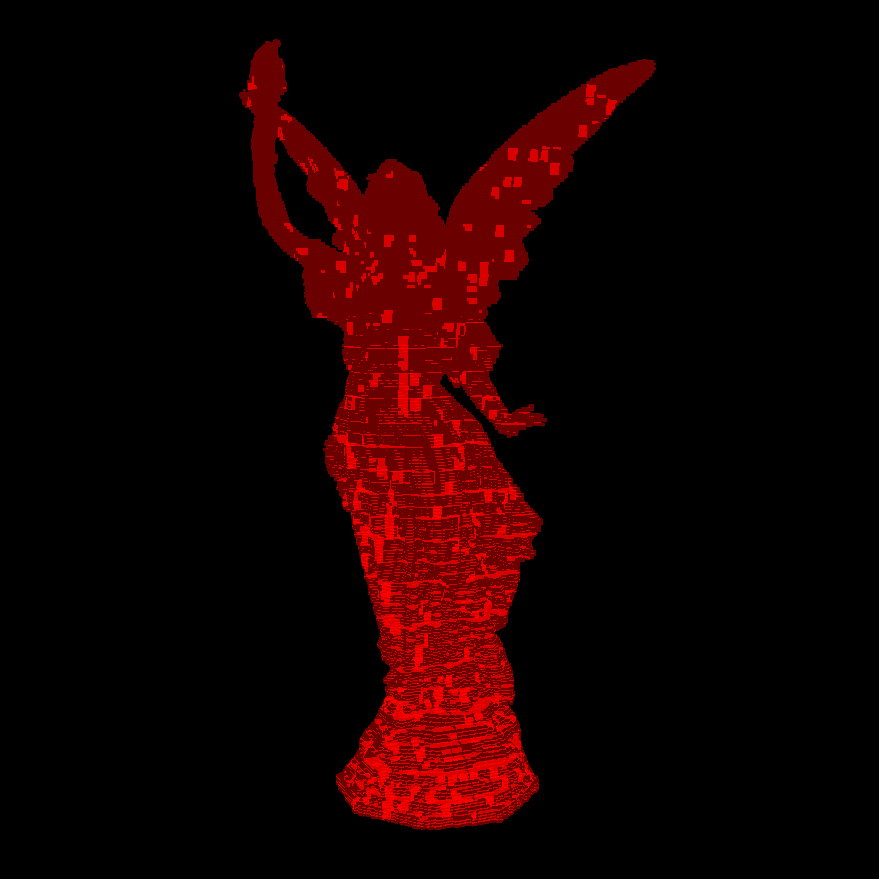
\includegraphics[height=100px]{images/graphics/overdraw-lucy1-pmoc.png}
  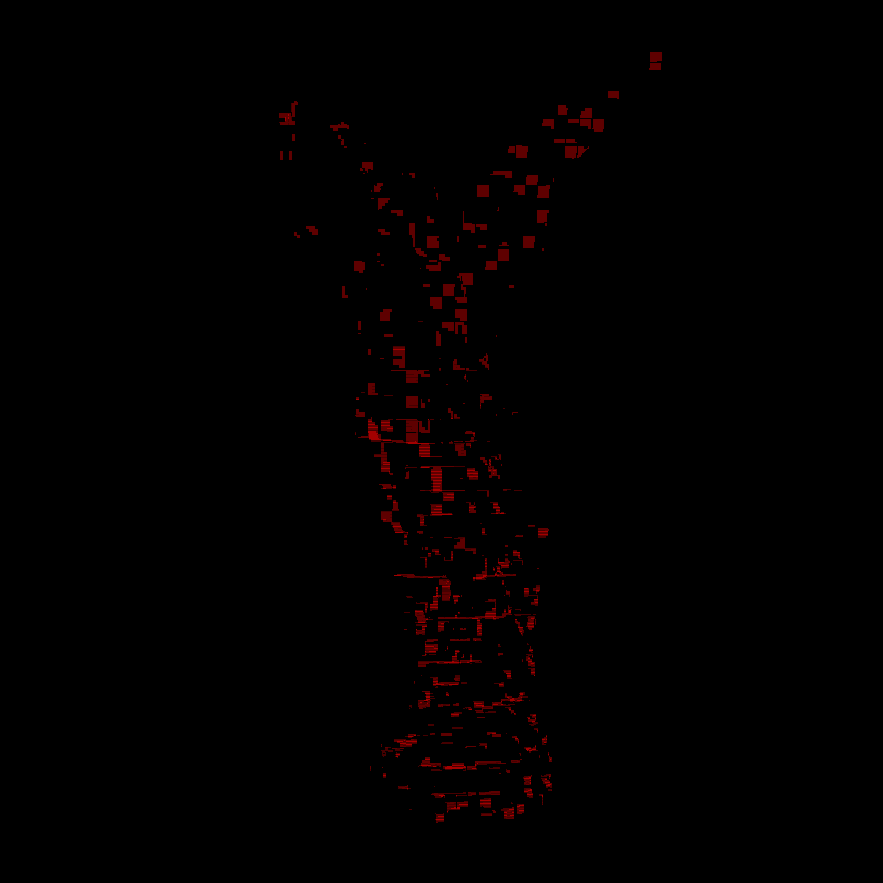
\includegraphics[height=100px]{images/graphics/overdraw-lucy1-diff.png}

  \begin{subfigure}{100px}
    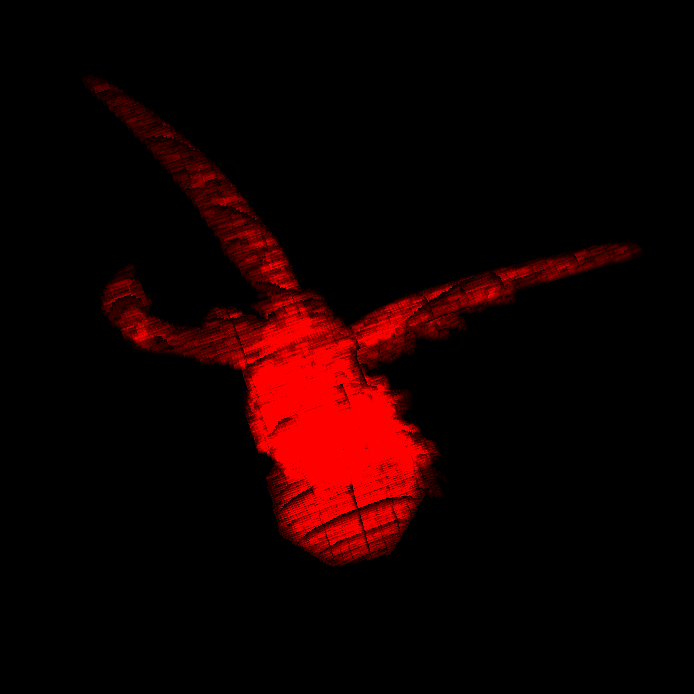
\includegraphics[height=100px]{images/graphics/overdraw-lucy2-nocull.png}
    \caption{}
    \parbox{\linewidth}{\centering\footnotesize No Occlusion\\Culling}
  \end{subfigure}
  \begin{subfigure}{100px}
    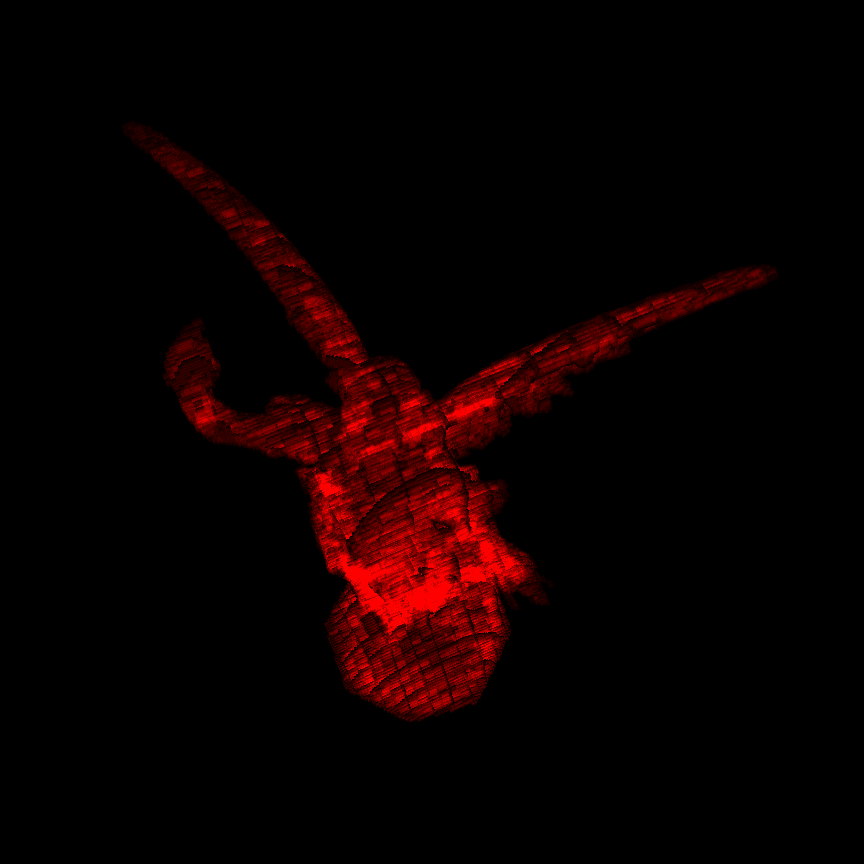
\includegraphics[height=100px]{images/graphics/overdraw-lucy2-pooc.png}
    \caption{}
    \parbox{\linewidth}{\centering\footnotesize Per-Octree Node\\Occlusion Culling}
  \end{subfigure}
  \begin{subfigure}{100px}
    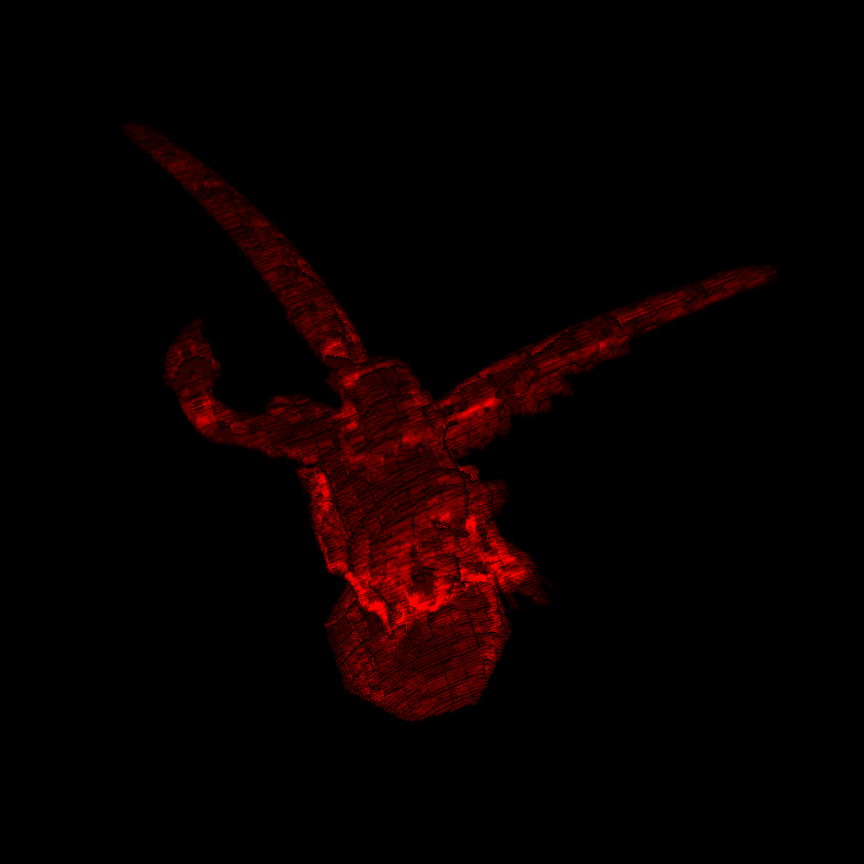
\includegraphics[height=100px]{images/graphics/overdraw-lucy2-pmoc.png}
    \caption{}
    \parbox{\linewidth}{\centering\footnotesize Per-Meshlet\\Occlusion Culling}
  \end{subfigure}
  \begin{subfigure}{100px}
    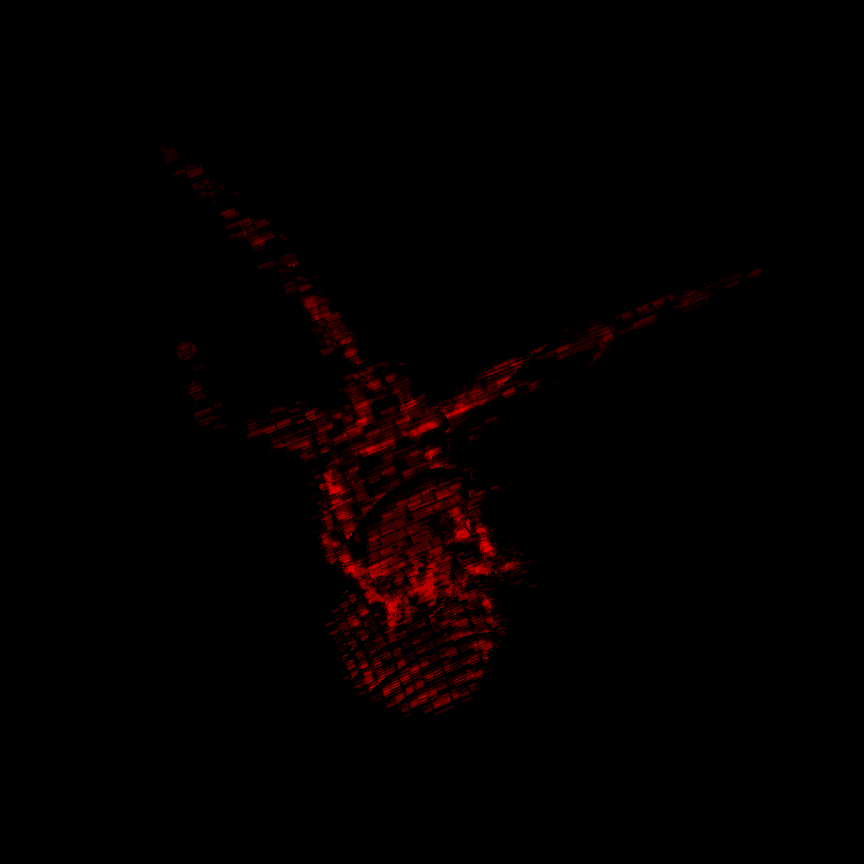
\includegraphics[height=100px]{images/graphics/overdraw-lucy2-diff.png}
    \caption{}
    \parbox{\linewidth}{\centering\footnotesize Difference\\(b) vs. (c)}
  \end{subfigure}

  \caption{Overdraw of the pixels from two different camera angles. 
  The image values are enhanced for better visualization.}
  \label{fig:lucy-overdraw}
\end{figure}

\noindent
Figure \ref{fig:lucy-overdraw} shows that the \ac{PONOC} had more 
overdrawn pixels than the \ac{PMOC} configuration. While the 
\ac{PONOC} resulted in a maximum overdraw of 38 draws per pixel, 
the \ac{PMOC} was able to reduce this to a maximum of 27 draws.
The comparison measurement without culling applied resulted in a maximum of 78 draws. 
The side view featured only a maximum of 7 draws per pixel in both configurations.


\clearpage




\subsection*{Stanford Bunny}

The \emph{Stanford Bunny} is a large and dense model with a lot of voxels in any possible resolution.
It also has different features to it, one of them being the curved surface, resulting in a lot of octree 
nodes not being filled completely. On the other hand, because of its large volume, the model is assumed 
to be efficient when rendering the best occluders, aggregating a lot of smaller octree nodes to larger 
approximations.

\subsubsection*{Culling Results} \label{subsubsec-culling-results-bunny}

% --------------------------------------- BUNNY 256 --------------------------------------

\begin{figure}[!htb]              % Bunny 256 Voxels Test Anim
    \begin{center}
      \begin{tikzpicture}
        \begin{axis}[
            width=\linewidth, % Scale the plot to \linewidth
            height=100px,
            xlabel={Frames},
            ylabel={VComputed Voxels},
            grid,
            xmin=0,
            xmax=1186,
            ymin=100000,
            ymax=500000,
            legend style={at={(0.5,1.7)}, anchor=north, legend columns=2},
          ]
          \addplot[blue, no marks, solid] table[col sep=comma, x=frame, x expr=\thisrow{frame} * 1186 / 1186, y=visible_voxels]{plotdata/bunny_256_voxels.csv};
          \addplot[blue, dotted, no marks, domain=0:1186, samples=50] {385210};
          \addplot[red, no marks, solid] table[col sep=comma, x=frame, x expr=\thisrow{frame} * 1186 / 1490, y=visible_voxels]{plotdata/bunny_256_voxels_pmoc.csv};
          \addplot[red, dotted, no marks, domain=0:1186, samples=50] {180266};
          \legend{Per-Octree Occlsion Culling, Per-Meshlet Occlusion Culling}
        \end{axis}
      \end{tikzpicture}

      \begin{tikzpicture}
        \begin{axis}[
            width=\linewidth, % Scale the plot to \linewidth
            height=100px,
            xlabel={Frames},
            ylabel={Computed Nodes},
            grid,
            xmin=0,
            xmax=1186,
            ymin=3000,
            ymax=10000,
            legend style={at={(0.5,1.7)}, anchor=north, legend columns=2},
          ]
          \addplot[blue, no marks, solid] table[col sep=comma, x=frame, x expr=\thisrow{frame} * 1186 / 1186, y=visible_nodes]{./plotdata/bunny_256_nodes.csv};
          \addplot[blue, dotted, no marks, domain=0:1186, samples=50] {8519};
          \addplot[red, no marks, solid] table[col sep=comma, x=frame, x expr=\thisrow{frame} * 1186 / 1490, y=visible_nodes]{./plotdata/bunny_256_nodes_pmoc.csv};
          \addplot[red, dotted, no marks, domain=0:1186, samples=50] {5415};
          \legend{Per-Octree Occlsion Culling, Per-Meshlet Occlusion Culling}
        \end{axis}
      \end{tikzpicture}

      \caption{First: The amount of visible voxels over the course of the test animation. 
      Second: The amount of visible octree nodes over the course of the test animation.}
      \label{plt:bunny-256-culling-res-voxels}
    \end{center}
  \end{figure}
% ----------------------------------------------------------------------------------------

\noindent
Similar to the first model, the \emph{Stanford Bunny} also discarded a significant amount of 
voxels in both of the applied culling configurations. The average culling ratio was $88.6\%$ 
for the \ac{PONOC} and $94.6\%$ for the per-meshlet culling. This immense 
amount of occlusion was due to the already large amount of \emph{3,379,738} total voxels in the 
mesh and the large volume of the model, which provided a good basis for the generation of the 
best occluders. \\


\noindent
The average amount of visible voxels was \emph{385,210} for \ac{PONOC}, which is 
marked as the blue dotted line, and \emph{180,266} for \ac{PMOC}, marked in red.
The average amount of visible octree nodes was \emph{8,519} for \ac{PONOC}, which 
is marked as the blue dotted line, and \emph{5,415} for \ac{PMOC}, which is marked
as the red dotted line.

\subsubsection*{CPU Performance Results} \label{subsubsec-cpu-performance-results-bunny}

\begin{figure}[!htb]              % Bunny cpu
  \begin{center}
    \begin{tikzpicture}
      \begin{axis}[
          width=\linewidth,
          height=100px,
          xlabel={Frames},
          ylabel={Update Time (s)},
          grid,
          xmin=0,
          xmax=1186,
          ymin=0,
          ymax=0.00005,
          legend style={at={(0.5,1.7)}, anchor=north, legend columns=2},
        ]
        \addplot[brown!60, no marks, solid] table[col sep=comma, x=frame, x expr=\thisrow{frame} * 1186 / 1236, y=time]{./plotdata/cpu/bunny_256_updateTime_nocull.csv};
        \addplot[blue, no marks, solid]  table[col sep=comma, x=frame, x expr=\thisrow{frame} * 1186 / 1574, y=time]{./plotdata/cpu/bunny_256_updateTime_pooc.csv};
        \addplot[red, no marks, solid] table[col sep=comma, x=frame, x expr=\thisrow{frame} * 1186 / 1700, y=time]{./plotdata/cpu/bunny_256_updateTime.csv};
        \legend{No Occlusion Culling, Per-Octree Occlsion Culling, Per-Meshlet Occlusion Culling}
      \end{axis}
    \end{tikzpicture}
    \begin{tikzpicture}
      \begin{axis}[
          width=\linewidth,
          height=100px,
          xlabel={Frames},
          ylabel={Render Time (s)},
          grid,
          xmin=0,
          xmax=1186,
          ymin=0,
          ymax=0.00025,
          legend style={at={(0.5,1.7)}, anchor=north, legend columns=2},
        ]
        \addplot[brown!60, no marks, solid] table[col sep=comma, x=frame, x expr=\thisrow{frame} * 1186 / 1236, y=time]{./plotdata/cpu/bunny_256_renderTime_nocull.csv};
        \addplot[blue, no marks, solid] table[col sep=comma, x=frame, x expr=\thisrow{frame} * 1186 / 1574, y=time]{./plotdata/cpu/bunny_256_renderTime_pooc.csv};
        \addplot[red, no marks, solid] table[col sep=comma, x=frame, x expr=\thisrow{frame} * 1186 / 1700, y=time]{./plotdata/cpu/bunny_256_renderTime.csv};
        \legend{No Occlusion Culling, Per-Octree Occlsion Culling, Per-Meshlet Occlusion Culling}
      \end{axis}
    \end{tikzpicture}
    \caption{Overview of the render times over the course of the test animation. The first graph shows the time 
    each frame took to execute the \emph{Update()} function on the \ac{CPU}. The second graph shows the time each 
    frame took to execute the function \emph{Render()} on the \ac{CPU}. This includes the completion of the 
    \ac{GPU} computations.}
    \label{plt:bunny-256-culling-cpu-time}
  \end{center}
\end{figure}


\noindent
Like with the \emph{Lucy} model, the \emph{Bunny} showed no significant difference in \ac{CPU} computation time. 
In Figure \ref{plt:bunny-256-culling-cpu-time}, the second graph shows a small amount of frames between frames 280 
and 380, which seem to have been faster in execution using the \ac{PMOC}. However, it is not 
obvious why there would be any difference here. Similarly, the first graph also shows small differences that are 
not considered significant enough to make any assumptions about them. Therefore, for this particular model, the 
\ac{CPU} compute times are also considered to be static between both configurations.

\subsubsection*{GPU Performance Results} \label{subsubsec-gpu-performance-results-bunny}

\begin{figure}[!htb]
  \centering
  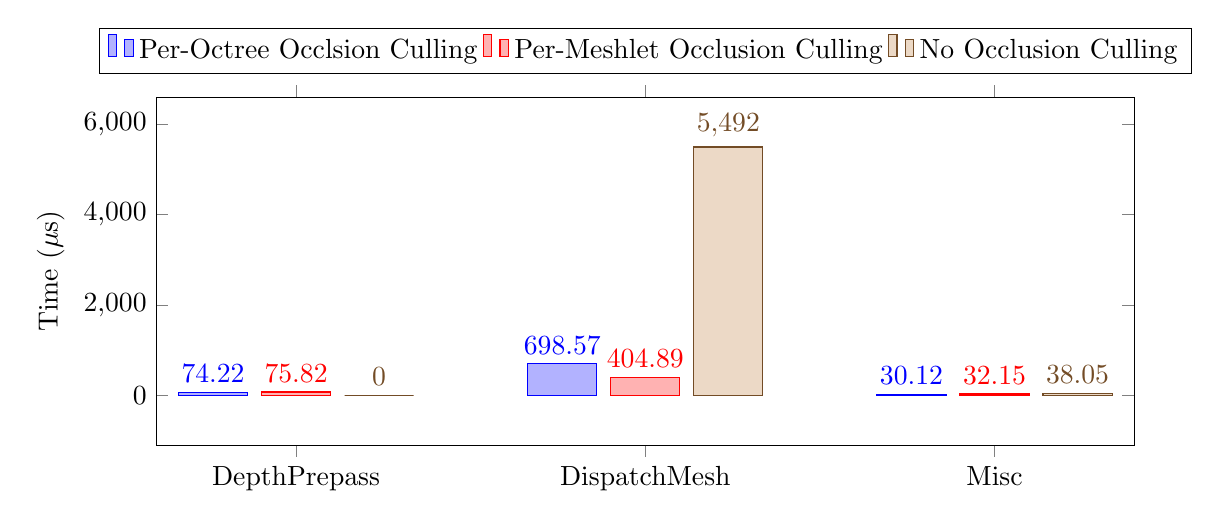
\begin{tikzpicture}
    \begin{axis}[
        height=6cm,
        width=14cm,
        x tick label style={/pgf/number format/1000 sep=},
        ylabel={Time ($\mu$s)},
        legend style={at={(0.5,1.2)}, anchor=north, legend columns=-1},
        symbolic x coords={DepthPrepass, DispatchMesh, Misc},
        xtick=data,
        ybar=0.4,
        bar width=25pt,
        ymin=0,
        nodes near coords,
        enlargelimits=0.2,
    ]
    \addplot+[bar shift=-30pt] coordinates {(DepthPrepass,74.22) (DispatchMesh,698.57) (Misc,30.12)};
    \addplot+[bar shift=0pt] coordinates {(DepthPrepass,75.82) (DispatchMesh,404.89) (Misc,32.1526)};
    \addplot+[bar shift=30pt] coordinates {(DepthPrepass,0) (DispatchMesh,5492.00) (Misc,38.0522)};
    \legend{Per-Octree Occlsion Culling, Per-Meshlet Occlusion Culling, No Occlusion Culling}
    \end{axis}
  \end{tikzpicture}

  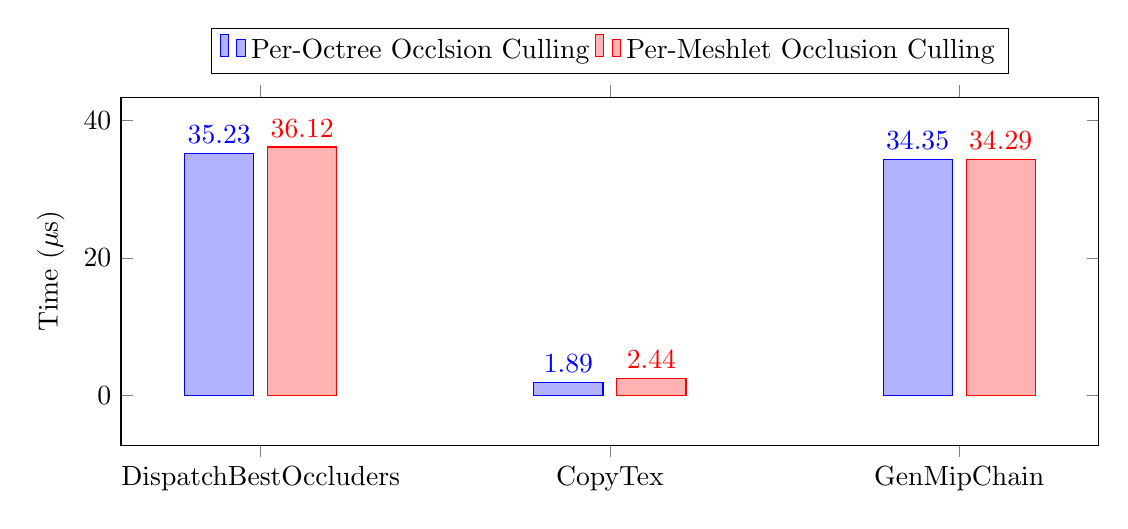
\begin{tikzpicture}
    \begin{axis}[
        height=6cm,
        width=14cm,
        x tick label style={/pgf/number format/1000 sep=},
        ylabel={Time ($\mu$s)},
        legend style={at={(0.5,1.2)}, anchor=north, legend columns=-1},
        symbolic x coords={DispatchBestOccluders, CopyTex, GenMipChain},
        xtick=data,
        ybar=0.4,
        bar width=25pt,
        ymin=0,
        nodes near coords,
        enlargelimits=0.2,
    ]
    \addplot+[bar shift=-15pt] coordinates {(DispatchBestOccluders,35.23) (CopyTex,1.89) (GenMipChain,34.35)};
    \addplot+[bar shift=15pt] coordinates {(DispatchBestOccluders,36.12) (CopyTex,2.44) (GenMipChain,34.29)};
    \legend{Per-Octree Occlsion Culling, Per-Meshlet Occlusion Culling}
    \end{axis}
  \end{tikzpicture}

  \caption{First: The complete time measured on the \ac{GPU}. The \emph{Depth Prepass} is the extra overhead 
  introduced by the \ac{HZB}. The \emph{Dispatch Mesh} is the drawing of the meshes, including the occlusion 
  culling. \emph{Miscellaneous} includes a small amount of \emph{Barriers} used for synchronisation and the 
  rendering of some debug \ac{UI}. It is considered to be more or less static in computation time and is not 
  part of the actual algorithm measured in this experiment. Second: The time measured in the \emph{Depth Prepass}. 
  The \emph{Dispatch Best Occluders} is the drawing to the depth buffer. The \emph{Copy Depth Buffer} computation 
  copies the depth buffers content into the final \ac{HiZ} resource. Finally, \emph{Generate HiZ Pyramid} 
  shows the \ac{HiZ} creation, which is done sequentially.}
\end{figure}

\noindent
The \ac{GPU} performance shows a significant difference when comparing both configurations. The per-meshlet 
occlusion culling was able to decrease the time spent on \emph{DispatchMesh} by $36.1\%$ on average as compared 
to the \ac{PONOC}. On closer inspection, the depth prepass showed a minor difference 
in runtime, similar to the prepass of the \emph{Lucy} model. The difference in runtime is 1.6 microseconds, 
mostly due to differences in \ac{HiZ} dispatch and depth buffer copy. \\

\noindent
Compared to the \emph{Lucy} model, the depth prepass took considerably longer to compute. This was mainly due to 
the longer dispatch of the best occluders, which took about three times as long. The \emph{Bunny}'s amount of 
best occluders was 5.1 times as high as the amount of best occluders in the \emph{Lucy} model.

\subsubsection*{Overdraw} \label{subsubsec-overdraw-bunny}

\begin{figure}[!htb]
  \centering
  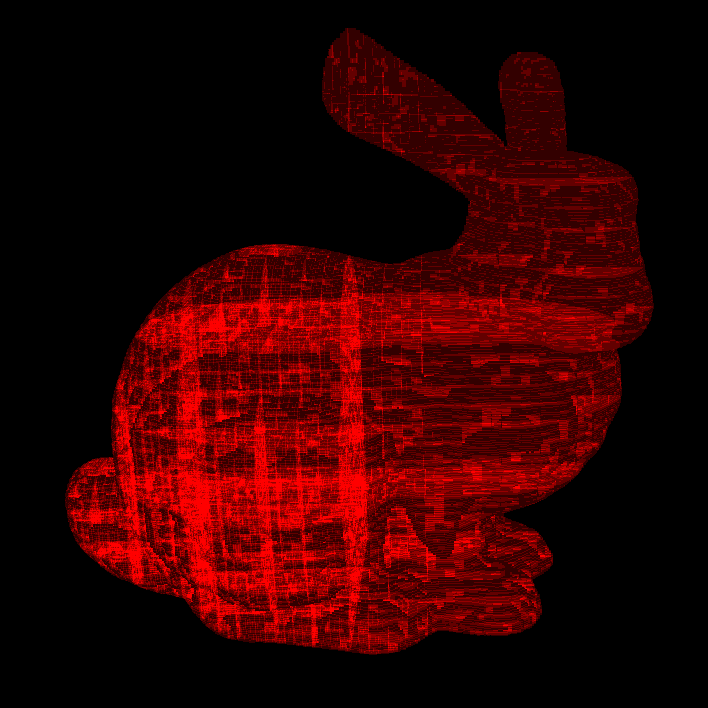
\includegraphics[width=100px]{images/graphics/overdraw-bunny1-nocull.png}
  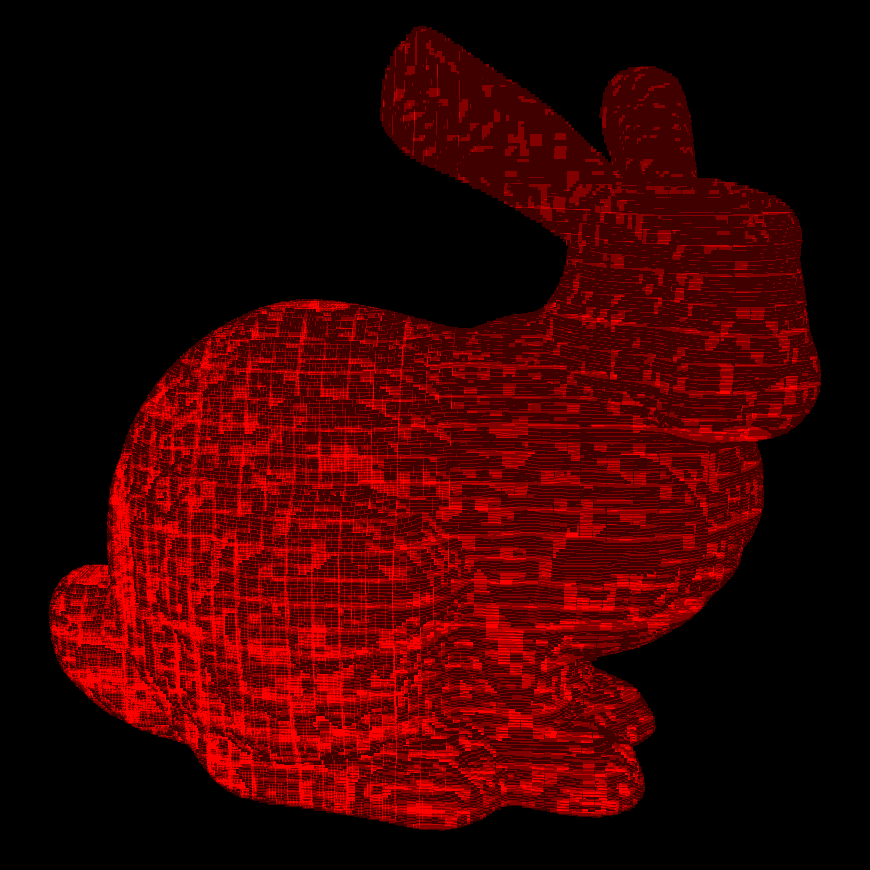
\includegraphics[width=100px]{images/graphics/overdraw-bunny1-pooc.png}
  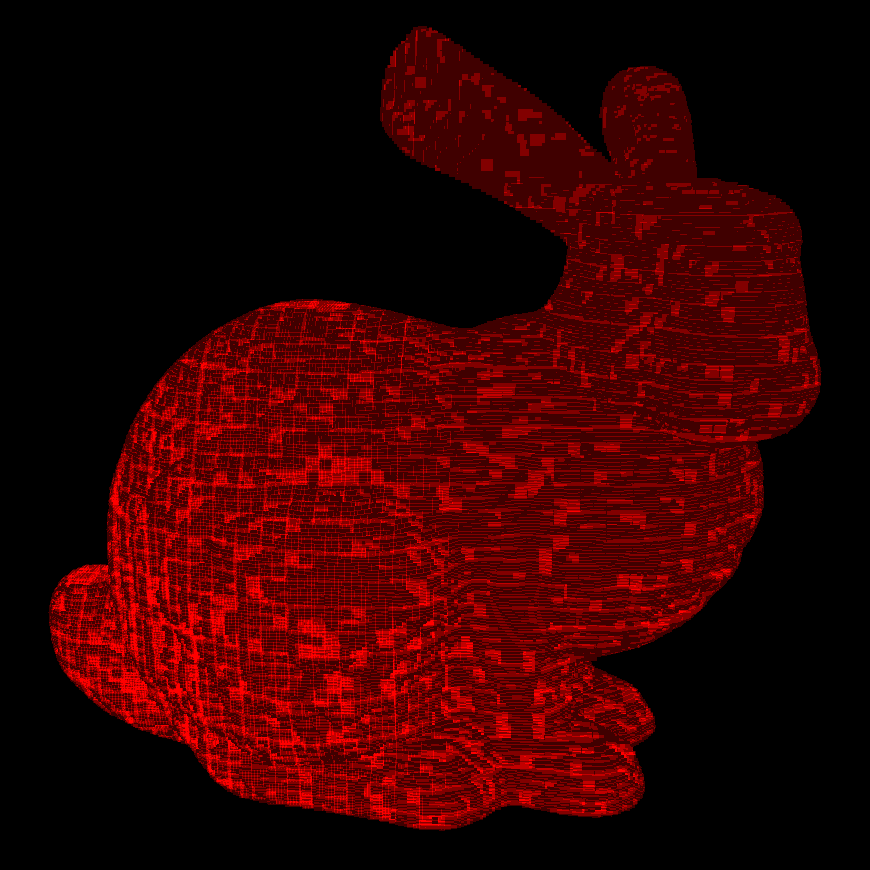
\includegraphics[width=100px]{images/graphics/overdraw-bunny1-pmoc.png}
  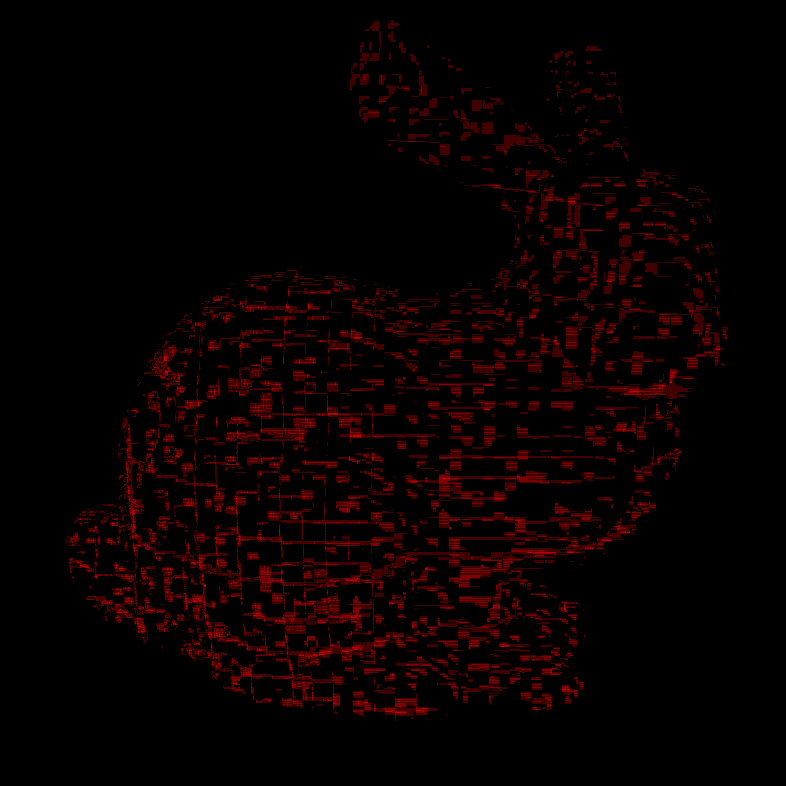
\includegraphics[width=100px]{images/graphics/overdraw-bunny1-diff.png}

  \begin{subfigure}{100px}
    
\includegraphics[width=100px]{images/graphics/overdraw-bunny2-nocull.png}
    \caption{}
    \parbox{\linewidth}{\centering\footnotesize No Occlusion\\Culling}
  \end{subfigure}
  \begin{subfigure}{100px}
    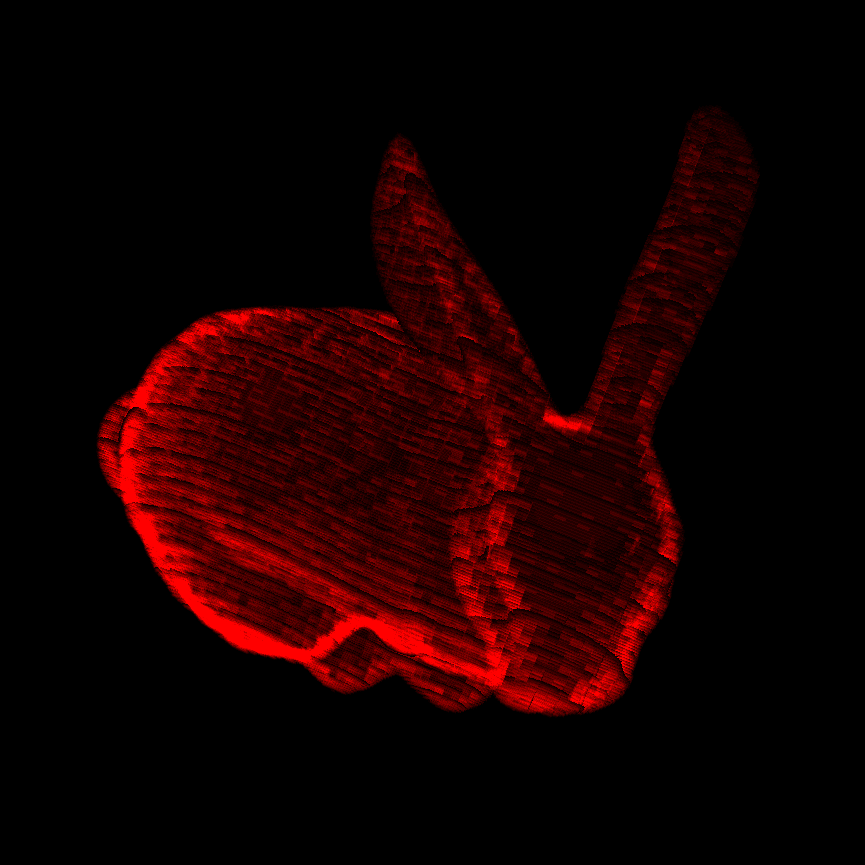
\includegraphics[width=100px]{images/graphics/overdraw-bunny2-pooc.png}
    \caption{}
    \parbox{\linewidth}{\centering\footnotesize Per-Octree Node\\Occlusion Culling}
  \end{subfigure}
  \begin{subfigure}{100px}
    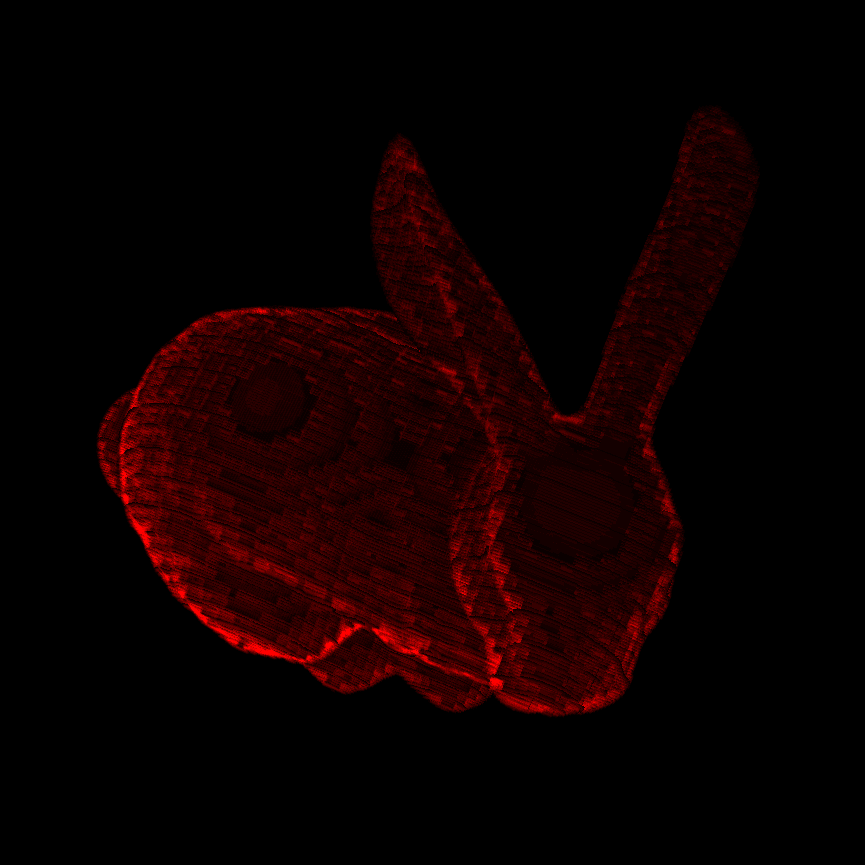
\includegraphics[width=100px]{images/graphics/overdraw-bunny2-pmoc.png}
    \caption{}
    \parbox{\linewidth}{\centering\footnotesize Per-Meshlet\\Occlusion Culling}
  \end{subfigure}
  \begin{subfigure}{100px}
    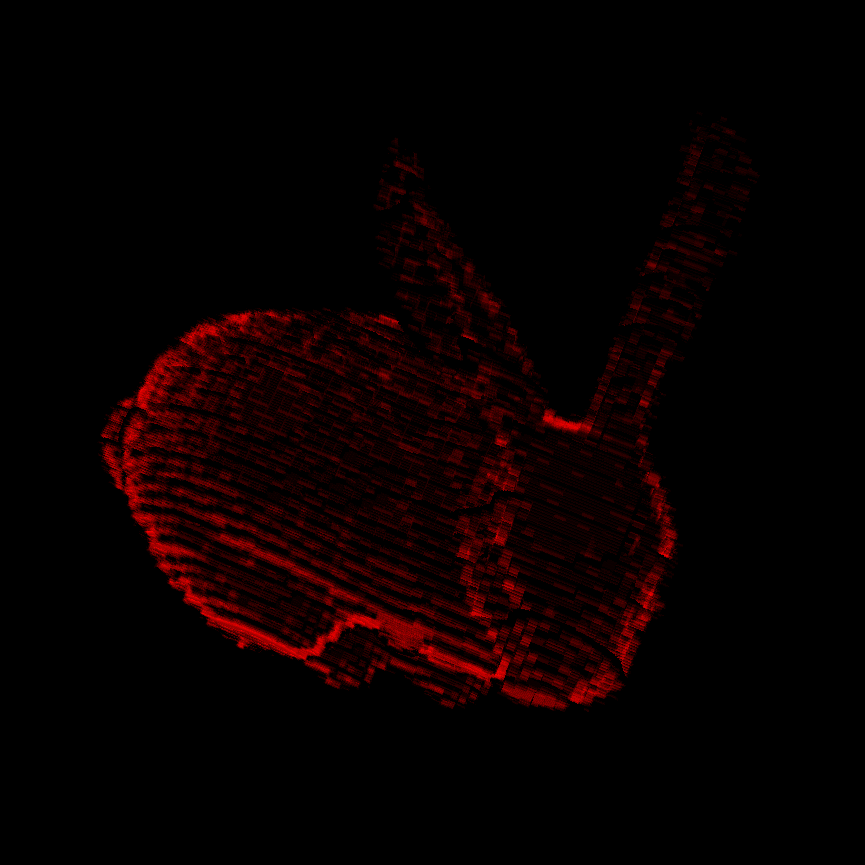
\includegraphics[width=100px]{images/graphics/overdraw-bunny2-diff.png}
    \caption{}
    \parbox{\linewidth}{\centering\footnotesize Difference\\(b) vs. (c)}
  \end{subfigure}

  \caption{Overdraw of the pixels from two different camera angles. 
  The image values are enhanced for better visualization.}
  \label{fig:bunny-overdraw}
\end{figure}

\noindent
Figure \ref{fig:bunny-overdraw} shows the overdraw of pixels from two different camera angles.
Both rows show that the \ac{PONOC} had more overdrawn pixels than the 
\ac{PMOC} configuration. The difference is in favor of per-meshlet 
culling, which had only a maximum of 43 draws to the same pixels as compared to 60 draws. Without 
the culling activated, the maximum amount of overdraw was measured to be 111 draws to the same pixel.
The camera angle clearly made a difference here, as the top view increased the amount of 
overdraw significantly. This is especially visible on the surface of the model, where a lot 
of rounded edges are present. \\

\noindent
The images also show how the per-octree node culling produces more overdraw on the surface than the 
per-meshlet culling because a larger portion of the voxels on the outside of the mesh were being 
culled. In Figure \ref{fig:bunny-overdraw}, this is visible as the broader red outline around the 
bunny.

\clearpage




\subsection*{Torus}

The \emph{Torus} provides a higher voxel count and a hole in it, which created an area where the 
octree isn't densely filled with voxels. This model was specifically used to test the algorithm's 
capabilities of culling voxels when the voxels were densely crowded in small parts of the scene and 
at the same time provided areas with no voxels at all. Also, the \emph{Torus} is an inherently round 
shape and therefore has a lot of partially filled octree nodes representing its surface. 

\subsubsection*{Culling Results} \label{subsubsec-culling-results-torus}

% --------------------------------------- TORUS 256 --------------------------------------

\begin{figure}[!htb]              % Torus 256 Voxels Test Anim
    \begin{center}
      \begin{tikzpicture}
        \begin{axis}[
            width=\linewidth, % Scale the plot to \linewidth
            height=100px,
            xlabel={Frames},
            ylabel={VComputed Voxels},
            grid,
            xmin=0,
            xmax=1087,
            ymin=70000,
            ymax=500000,
            legend style={at={(0.5,1.7)}, anchor=north, legend columns=2},
          ]
          \addplot[blue, no marks, solid] table[col sep=comma, x=frame, x expr=\thisrow{frame} * 1087 / 1087, y=visible_voxels]{./plotdata/torus_256_voxels.csv};
          \addplot[blue, dotted, no marks, domain=0:1087, samples=50] {359313};
          \addplot[red, no marks, solid] table[col sep=comma, x=frame, x expr=\thisrow{frame} * 1087 / 1845, y=visible_voxels]{./plotdata/torus_256_voxels_pmoc.csv};
          \addplot[red, dotted, no marks, domain=0:1087, samples=50] {170772};
          \legend{Per-Octree Occlsion Culling, Per-Meshlet Occlusion Culling}
        \end{axis}
      \end{tikzpicture}

      \begin{tikzpicture}
        \begin{axis}[
            width=\linewidth, % Scale the plot to \linewidth
            height=100px,
            xlabel={Frames},
            ylabel={Computed Nodes},
            grid,
            xmin=0,
            xmax=1087,
            ymin=1000,
            ymax=10000,
            legend style={at={(0.5,1.7)}, anchor=north, legend columns=2},
          ]
          \addplot[blue, no marks, solid] table[col sep=comma, x=frame, x expr=\thisrow{frame} * 1087 / 1087, y=visible_nodes]{./plotdata/torus_256_nodes.csv};
          \addplot[blue, dotted, no marks, domain=0:1087, samples=50] {7712};
          \addplot[red, no marks, solid] table[col sep=comma, x=frame, x expr=\thisrow{frame} * 1087 / 1845, y=visible_nodes]{./plotdata/torus_256_nodes_pmoc.csv};
          \addplot[red, dotted, no marks, domain=0:1087, samples=50] {4768};
          \legend{Per-Octree Occlsion Culling, Per-Meshlet Occlusion Culling}
        \end{axis}
      \end{tikzpicture}

      \caption{First: The amount of visible voxels over the course of the test animation. 
      Second: The amount of visible octree nodes over the course of the test animation.}
      \label{plt:torus-256-culling-res-voxels}
    \end{center}
  \end{figure}

% ----------------------------------------------------------------------------------------

\noindent
The \emph{Torus} model varied in culling efficiency depending on the view angle. As expected, the hole 
in the mesh turned out to be inefficient for the culling algorithm. When considering the occlusion ratio, 
both the \ac{PONOC} and the \ac{PMOC} performed significantly better 
when the torus was viewed from an angle, so the hole in the middle was occluded. The variation between 
the maximum amount of visible voxels and the minimum amount of voxels was the highest for the \emph{Torus} 
model, which is remarkable compared to the other models. Using this particular experimental setup, the 
lowest amount of visible voxels was $36.8\%$ of the maximum amount of visible voxels. This variation is 
also clearly evident in Figure \ref{plt:torus-256-culling-res-voxels}. \\ 

\noindent
In general, for per-octree culling, the average culling ratio was $84.4\%$, and $92.6\%$ for per-meshlet culling. 

\subsubsection*{CPU Performance Results} \label{subsubsec-cpu-performance-results-torus}

Similar to the other models, the \emph{Torus} showed very similar \ac{CPU} performances in both 
occlusion culling configurations. The measurements confirmed what could already be shown for the 
\emph{Bunny}: The time spent on the depth prepass directly correlates to the amount of best occluders 
for a given model.


\begin{figure}[!htb]              % Torus CPU times
  \begin{center}
    \begin{tikzpicture}
      \begin{axis}[
          width=\linewidth,
          height=100px,
          xlabel={Frames},
          ylabel={Update Time (s)},
          grid,
          xmin=0,
          xmax=1087,
          ymin=0,
          ymax=0.00005,
          legend style={at={(0.5,1.7)}, anchor=north, legend columns=2},
        ]
        \addplot[brown!60, no marks, solid] table[col sep=comma, x=frame, x expr=\thisrow{frame} * 1087 / 1262, y=time]{./plotdata/cpu/torus_256_updateTime_nocull.csv};
        \addplot[blue, no marks, solid] table[col sep=comma, x=frame, x expr=\thisrow{frame} * 1554 / 1863, y=time]{./plotdata/cpu/torus_256_updateTime_pooc.csv};
        \addplot[red, no marks, solid] table[col sep=comma, x=frame, x expr=\thisrow{frame} * 1087 / 1785, y=time]{./plotdata/cpu/torus_256_updateTime.csv};
        \legend{No Occlusion Culling, Per-Octree Occlsion Culling, Per-Meshlet Occlusion Culling}
      \end{axis}
    \end{tikzpicture}
    \begin{tikzpicture}
      \begin{axis}[
          width=\linewidth,
          height=100px,
          xlabel={Frames},
          ylabel={Render Time (s)},
          grid,
          xmin=0,
          xmax=1087,
          ymin=0,
          ymax=0.00025,
          legend style={at={(0.5,1.7)}, anchor=north, legend columns=2},
        ]
        \addplot[brown!60, no marks, solid] table[col sep=comma, x=frame, x expr=\thisrow{frame} * 1087 / 1262, y=time]{./plotdata/cpu/torus_256_renderTime_nocull.csv};
        \addplot[blue, no marks, solid] table[col sep=comma, x=frame, x expr=\thisrow{frame} * 1087 / 1554, y=time]{./plotdata/cpu/torus_256_renderTime_pooc.csv};
        \addplot[red, no marks, solid] table[col sep=comma, x=frame, x expr=\thisrow{frame} * 1087 / 1785, y=time]{./plotdata/cpu/torus_256_renderTime.csv};
        \legend{No Occlusion Culling, Per-Octree Occlsion Culling, Per-Meshlet Occlusion Culling}
      \end{axis}
    \end{tikzpicture}
    \caption{Overview of the render times over the course of the test animation. The upper graph shows the time 
    each frame took to execute the \emph{Update()} function on the \ac{CPU}. The lower graph shows the time each 
    frame took to execute the function \emph{Render()} on the \ac{CPU}. This includes the completion of the 
    \ac{GPU} computations.}
    \label{plt:torus-256-culling-cpu-time}
  \end{center}
\end{figure}

\subsubsection*{GPU Performance Results} \label{subsubsec-gpu-performance-results-torus}

The \ac{GPU} performance for the \emph{Torus} model was considerably better using the per-meshlet 
occlusion culling approach. While the depth prepass differed by only 0.54 microseconds in favor of the 
\ac{PONOC}, the complete time spent on the \ac{GPU} was decreased by $36.8\%$ 
using the \ac{PMOC} configuration as shown in Figure \ref{fig:torus-gpu-results}.

\begin{figure}[!htb]              % Torus GPU times
  \centering
  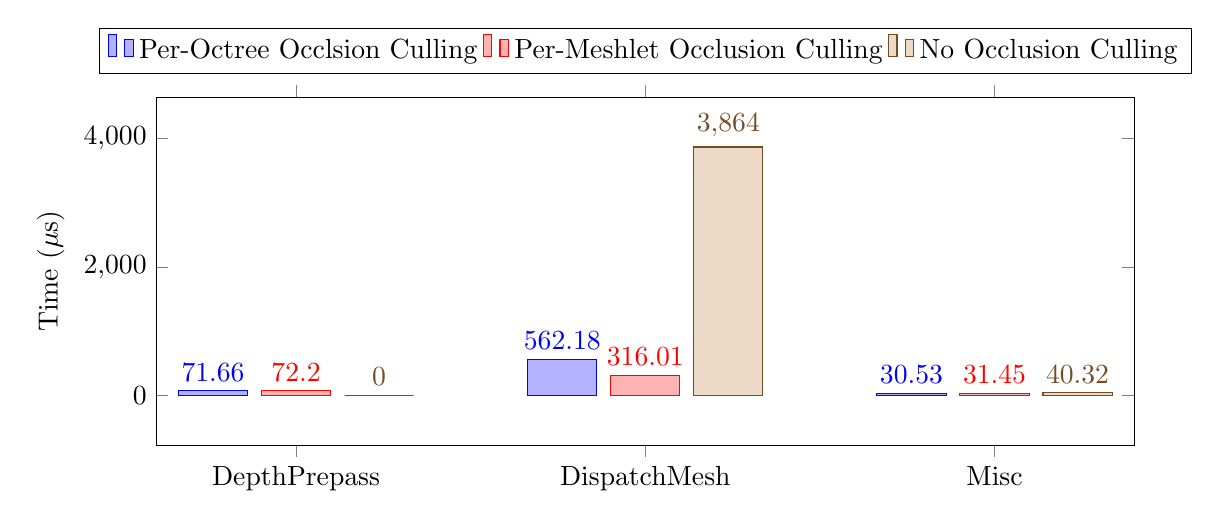
\begin{tikzpicture}
    \begin{axis}[
        height=6cm,
        width=14cm,
        x tick label style={/pgf/number format/1000 sep=},
        ylabel={Time ($\mu$s)},
        legend style={at={(0.5,1.2)}, anchor=north, legend columns=-1},
        symbolic x coords={DepthPrepass, DispatchMesh, Misc},
        xtick=data,
        ybar=0.4,
        bar width=25pt,
        ymin=0,
        nodes near coords,
        enlargelimits=0.2,
    ]
    \addplot+[bar shift=-30pt] coordinates {(DepthPrepass,71.66) (DispatchMesh,562.18) (Misc,30.53)};
    \addplot+[bar shift=0pt] coordinates {(DepthPrepass,72.20) (DispatchMesh,316.01) (Misc,31.4482)};
    \addplot+[bar shift=30pt] coordinates {(DepthPrepass,0) (DispatchMesh,3864.0) (Misc,40.31696)};
    \legend{Per-Octree Occlsion Culling, Per-Meshlet Occlusion Culling, No Occlusion Culling}
    \end{axis}
  \end{tikzpicture}

  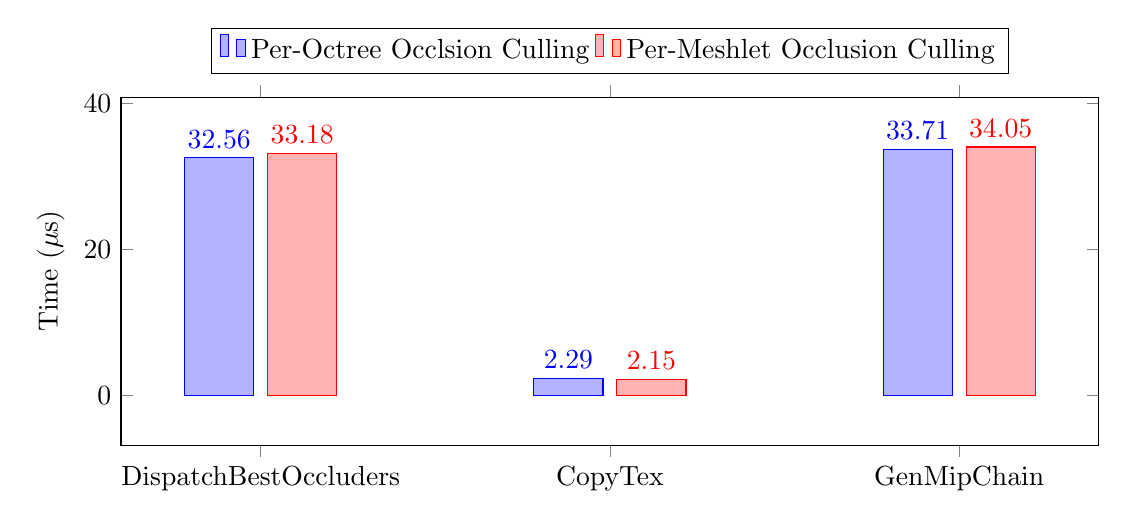
\begin{tikzpicture}
    \begin{axis}[
        height=6cm,
        width=14cm,
        x tick label style={/pgf/number format/1000 sep=},
        ylabel={Time ($\mu$s)},
        legend style={at={(0.5,1.2)}, anchor=north, legend columns=-1},
        symbolic x coords={DispatchBestOccluders, CopyTex, GenMipChain},
        xtick=data,
        ybar=0.4,
        bar width=25pt,
        ymin=0,
        nodes near coords,
        enlargelimits=0.2,
    ]
    \addplot+[bar shift=-15pt] coordinates {(DispatchBestOccluders,32.56) (CopyTex,2.29) (GenMipChain,33.71)};
    \addplot+[bar shift=15pt] coordinates {(DispatchBestOccluders,33.18) (CopyTex,2.15) (GenMipChain,34.05)};
    \legend{Per-Octree Occlsion Culling, Per-Meshlet Occlusion Culling}
    \end{axis}
  \end{tikzpicture}
  \caption{First: The complete time measured on the \ac{GPU}. The \emph{Depth Prepass} is the extra overhead 
  introduced by the \ac{HZB}. The \emph{Dispatch Mesh} is the drawing of the meshes, including the occlusion 
  culling. \emph{Miscellaneous} includes a small amount of \emph{Barriers} used for synchronisation and the 
  rendering of some debug \ac{UI}. It is considered to be more or less static in computation time and is not 
  part of the actual algorithm measured in this experiment. Second: The time measured in the \emph{Depth Prepass}. 
  The \emph{Dispatch Best Occluders} is the drawing to the depth buffer. The \emph{Copy Depth Buffer} computation 
  copies the depth buffers content into the final \ac{HiZ} resource. Finally, \emph{Generate HiZ Pyramid} shows 
  the \ac{HiZ} creation, which is done sequentially.}
  \label{fig:torus-gpu-results}
\end{figure}

\subsubsection*{Overdraw}

\begin{figure}[!htb]
  \centering
  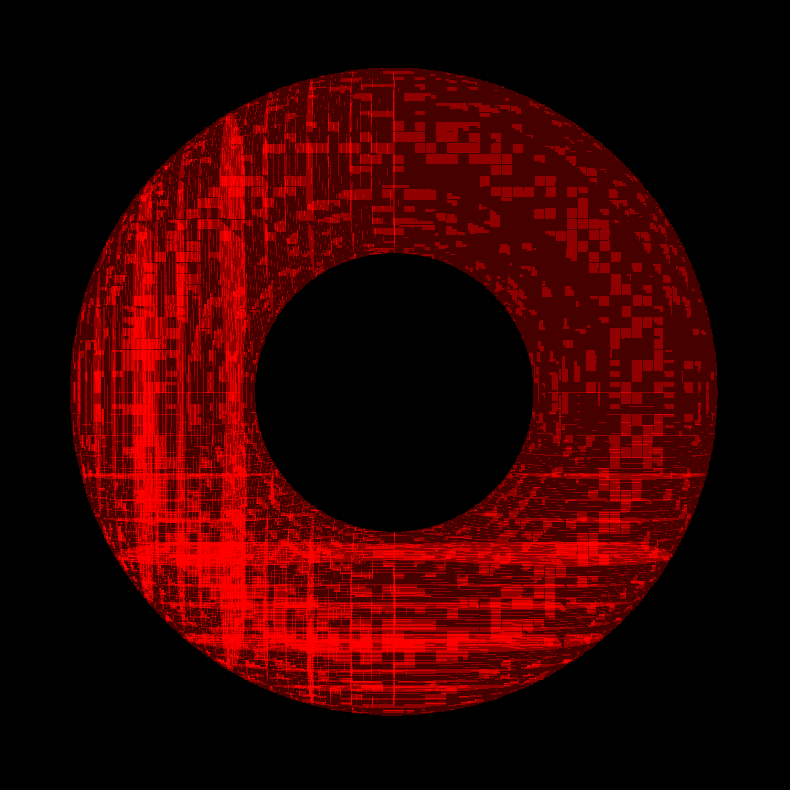
\includegraphics[height=100px]{images/graphics/overdraw-torus1-nocull.png}
  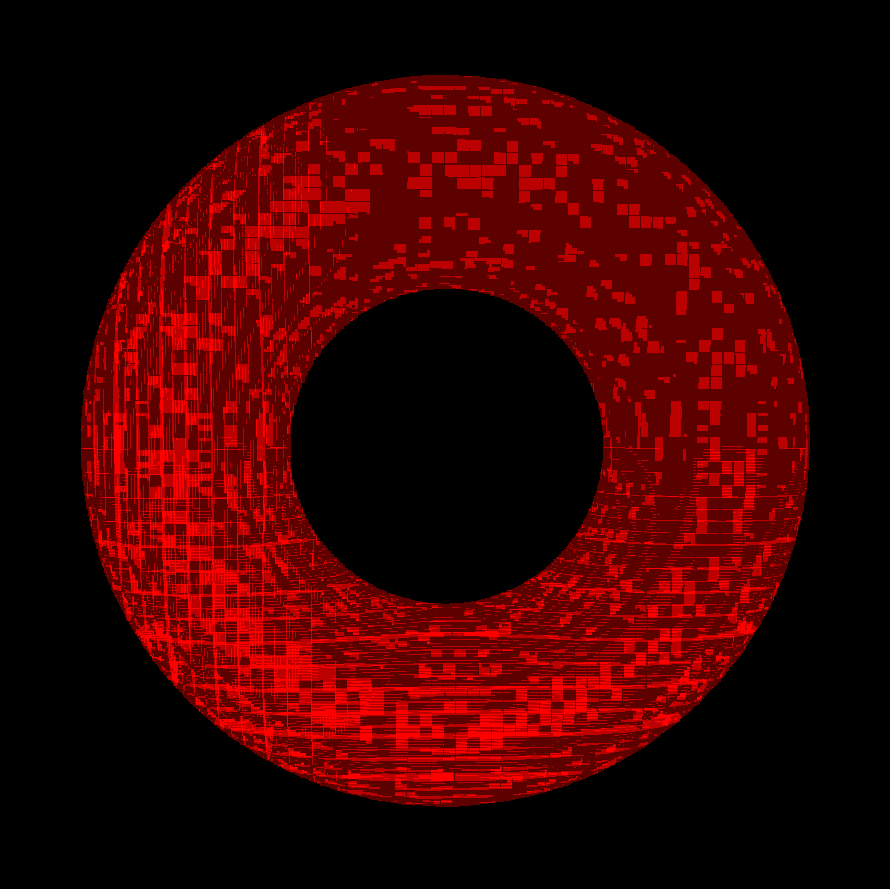
\includegraphics[height=100px]{images/graphics/overdraw-torus1-pooc.png}
  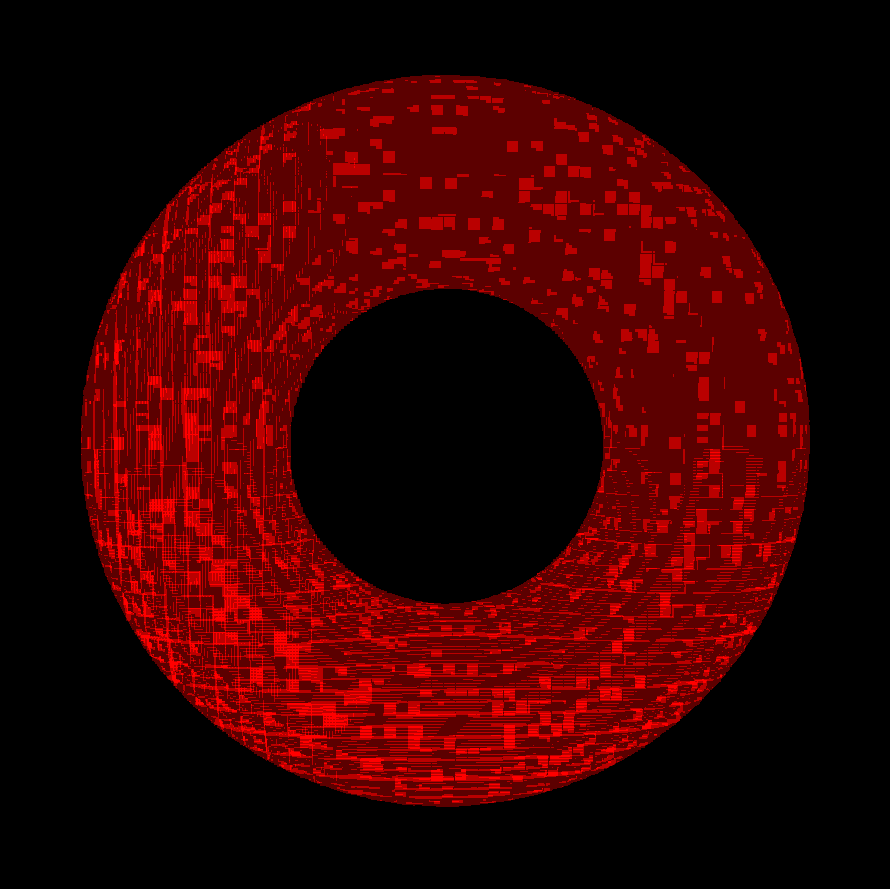
\includegraphics[height=100px]{images/graphics/overdraw-torus1-pmoc.png}
  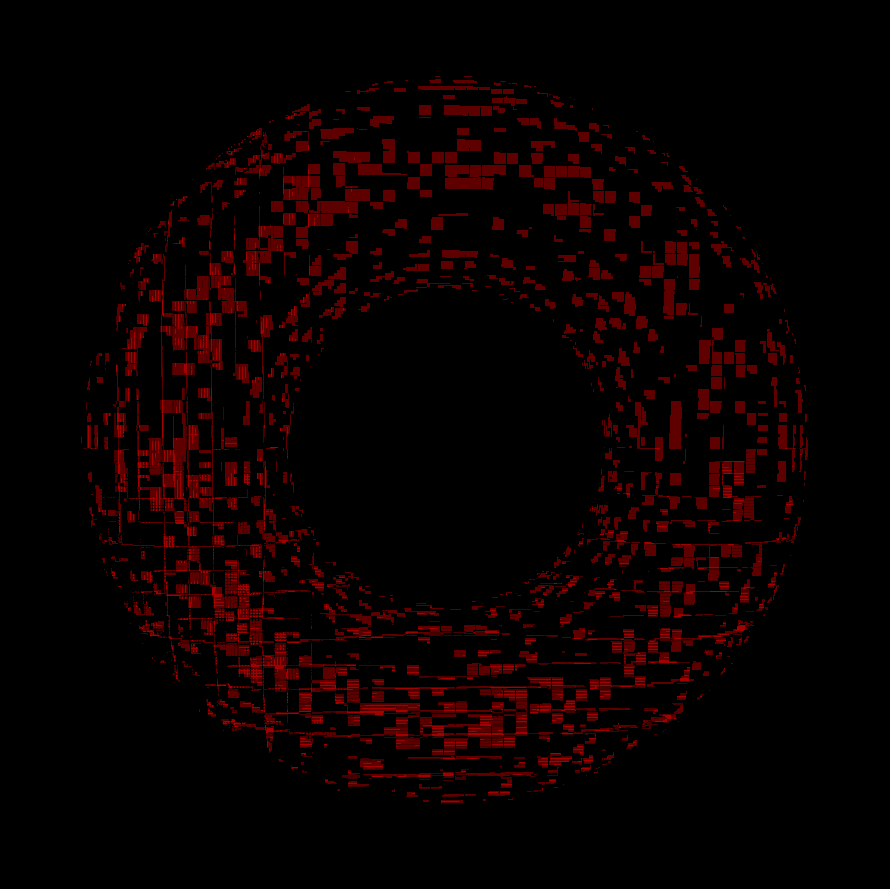
\includegraphics[height=100px]{images/graphics/overdraw-torus1-diff.png}

  \begin{subfigure}{100px}
    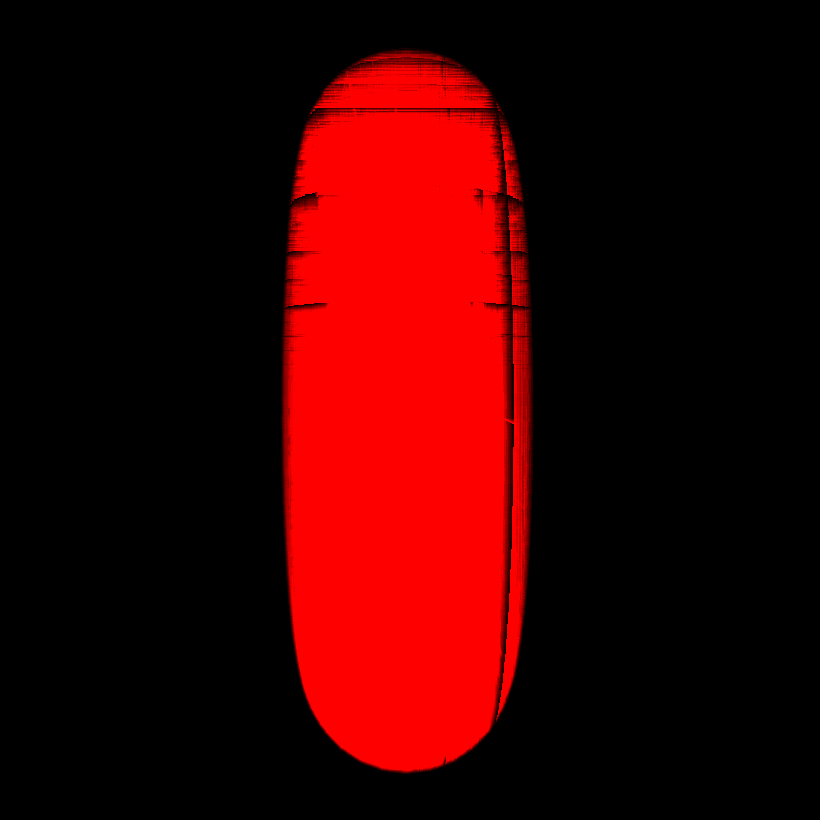
\includegraphics[height=100px]{images/graphics/overdraw-torus2-nocull.png}
    \caption{}
    \parbox{\linewidth}{\centering\footnotesize No Occlusion\\Culling}
  \end{subfigure}
  \begin{subfigure}{100px}
    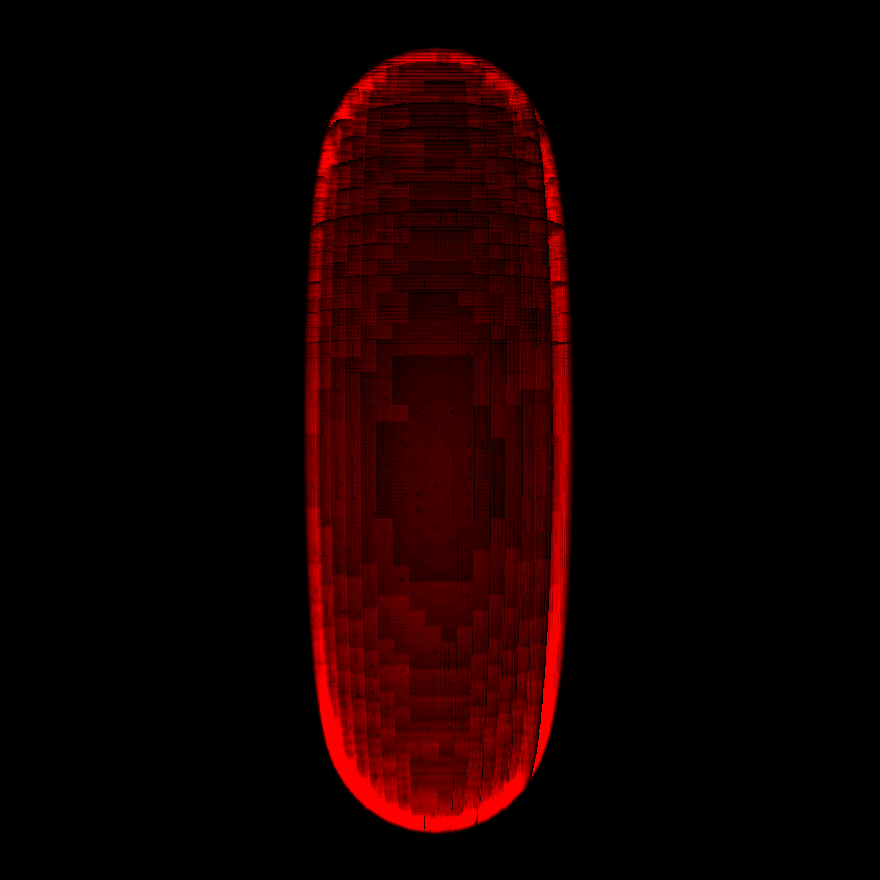
\includegraphics[height=100px]{images/graphics/overdraw-torus2-pooc.png}
    \caption{}
    \parbox{\linewidth}{\centering\footnotesize Per-Octree Node\\Occlusion Culling}
  \end{subfigure}
  \begin{subfigure}{100px}
    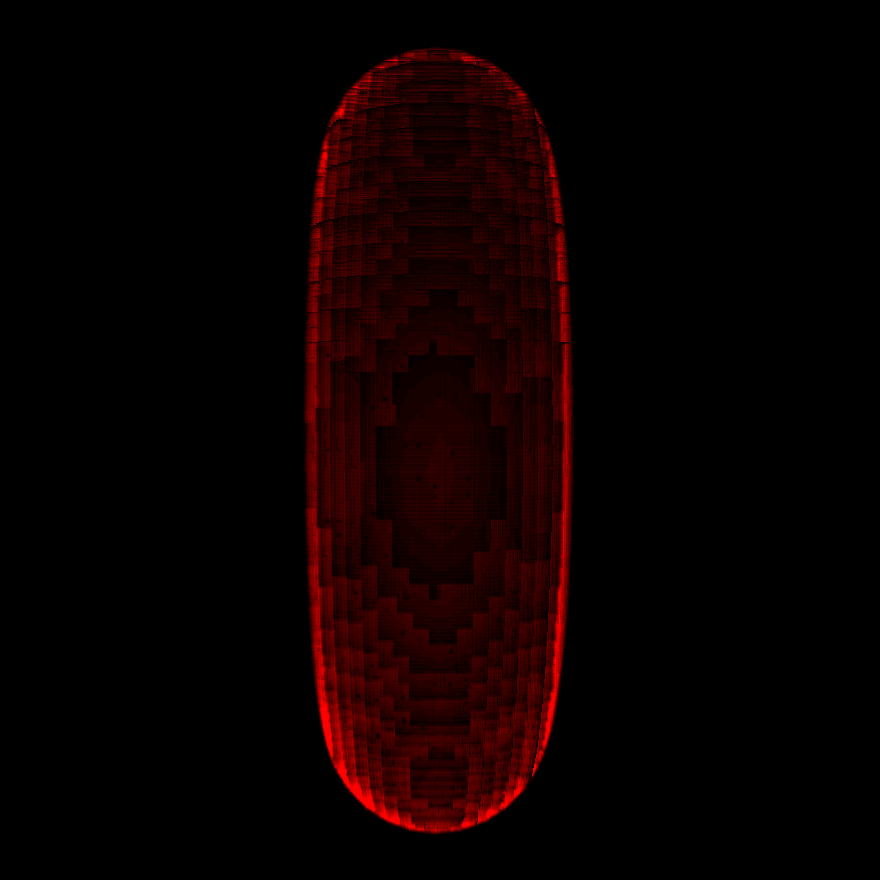
\includegraphics[height=100px]{images/graphics/overdraw-torus2-pmoc.png}
    \caption{}
    \parbox{\linewidth}{\centering\footnotesize Per-Meshlet\\Occlusion Culling}
  \end{subfigure}
  \begin{subfigure}{100px}
    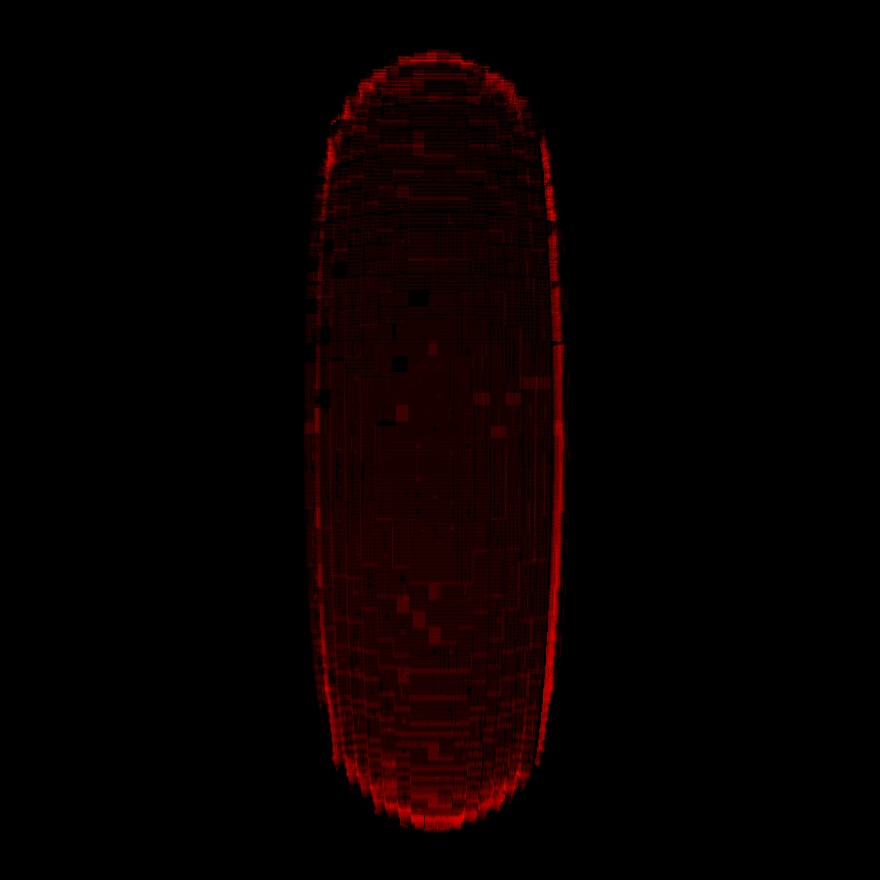
\includegraphics[height=100px]{images/graphics/overdraw-torus2-diff.png}
    \caption{}
    \parbox{\linewidth}{\centering\footnotesize Difference\\(b) vs. (c)}
  \end{subfigure}

  \caption{Overdraw of the pixels from two different camera angles. 
  The image values are enhanced for better visualization.}
  \label{fig:torus-overdraw}
\end{figure}

\noindent
Figure \ref{fig:torus-overdraw} shows the overdraw for the \emph{Torus} model from two 
camera perspectives. Clearly, the \ac{PMOC} configuration resulted 
in less overdraw, especially when viewed from the sides. As the second row of figure 
\ref{fig:torus-overdraw} shows, the edges were particularly overdrawn because of the 
missing depth information. Without culling, the maximum amount of overdraw was measured 
to be 267 draws to one pixel.


\clearpage




\subsection*{Terrain}

The \emph{Terrain} model aimed to replicate a relatively flat, open area that could be found in actual 
games like \emph{Minecraft}. Its surface is setup in a way that allows for only a small amount of best 
occluders to be formed. The terrain's hills are assumed to be occluding a large part of the scene, 
which again would help for rendering such a scene in a game.

\subsubsection*{Culling Results} \label{subsubsec-culling-results-terrain}

% -------------------------------------- TERRAIN 256 -------------------------------------

\begin{figure}[!htb]              % Terrain 256 Voxels Test Anim
    \begin{center}
      \begin{tikzpicture}
        \begin{axis}[
            width=\linewidth, % Scale the plot to \linewidth
            height=100px,
            xlabel={Frames},
            ylabel={VComputed Voxels},
            grid,
            xmin=0,
            xmax=1239,
            ymin=70000,
            ymax=500000,
            legend style={at={(0.5,1.7)}, anchor=north, legend columns=2},
          ]
          \addplot[blue, no marks, solid] table[col sep=comma, x=frame, x expr=\thisrow{frame} * 1239 / 1239, y=visible_voxels]{./plotdata/terrain_256_voxels.csv};
          \addplot[blue, dotted, no marks, domain=0:1239, samples=50] {396228};
          \addplot[red, no marks, solid] table[col sep=comma, x=frame, x expr=\thisrow{frame} * 1239 / 1759, y=visible_voxels]{./plotdata/terrain_256_voxels_pmoc.csv};
          \addplot[red, dotted, no marks, domain=0:1239, samples=50] {180440};
          \legend{Per-Octree Occlsion Culling, Per-Meshlet Occlusion Culling}

        \end{axis}
      \end{tikzpicture}

      \begin{tikzpicture}
        \begin{axis}[
            width=\linewidth, % Scale the plot to \linewidth
            height=100px,
            xlabel={Frames},
            ylabel={Computed Nodes},
            grid,
            xmin=0,
            xmax=1239,
            ymin=1000,
            ymax=10000,
            legend style={at={(0.5,1.7)}, anchor=north, legend columns=2},
          ]
          \addplot[blue, no marks, solid] table[col sep=comma, x=frame, x expr=\thisrow{frame} * 1239 / 1239, y=visible_nodes]{./plotdata/terrain_256_nodes.csv};
          \addplot[blue, dotted, no marks, domain=0:1239, samples=50] {8207};
          \addplot[red, no marks, solid] table[col sep=comma, x=frame, x expr=\thisrow{frame} * 1239 / 1759, y=visible_nodes]{./plotdata/terrain_256_nodes_pmoc.csv};
          \addplot[red, dotted, no marks, domain=0:1239, samples=50] {3832};
          \legend{Per-Octree Occlsion Culling, Per-Meshlet Occlusion Culling}

        \end{axis}
      \end{tikzpicture}

      \caption{First: The amount of visible voxels over the course of the test animation. 
      Second: The amount of visible octree nodes over the course of the test animation.}
      \label{plt:terrain-256-culling-res-voxels}
    \end{center}
  \end{figure}

% ----------------------------------------------------------------------------------------

\noindent
The \emph{Terrain} model showed a rather stable occlusion over time, with a ratio of about $58.4\%$ culled voxels 
using the per-octree culling configuration and about $81.1\%$ voxels being culled on average in the per-meshlet 
configuration. It was essential that the model in question had a minimal volume to it so the best occluders could 
be found and computed. \\

\noindent
The average amount of visible voxels was \emph{396,228} for \ac{PONOC}, which is marked as the 
blue dotted line, and \emph{180,440} for \ac{PMOC}, marked in red. The average amount of 
visible octree nodes was \emph{8,207} for \ac{PONOC}, which is marked as the blue dotted line, 
and \emph{3,832} for \ac{PMOC}, which is marked as the red dotted line.

\subsubsection*{CPU Performance Results} \label{subsubsec-cpu-performance-results-terrain}

Figure \ref{plt:terrain-256-culling-cpu-time} shows the \ac{CPU} performance over time, which in general 
resembles similar results as the other models discussed earlier. Again, there were a couple of frames that 
showed differences in frame time, although this could not be reliably attributed to any of the differences in 
the measured algorithm. 

\begin{figure}[!htb]              % Terrain CPU times
  \begin{center}
    \begin{tikzpicture}
      \begin{axis}[
          width=\linewidth,
          height=100px,
          xlabel={Frames},
          ylabel={Update Time (s)},
          grid,
          xmin=0,
          xmax=1239,
          ymin=0,
          ymax=0.00005,
          legend style={at={(0.5,1.7)}, anchor=north, legend columns=2},
        ]
        \addplot[brown!60, no marks, solid] table[col sep=comma, x=frame, x expr=\thisrow{frame} * 1239 / 1381, y=time]{./plotdata/cpu/terrain_256_updateTime_nocull.csv};
        \addplot[blue, no marks, solid] table[col sep=comma, x=frame, x expr=\thisrow{frame} * 1239 / 1572, y=time]{./plotdata/cpu/terrain_256_updateTime_pooc.csv};
        \addplot[red, no marks, solid] table[col sep=comma, x=frame, x expr=\thisrow{frame} * 1239 / 1813, y=time]{./plotdata/cpu/terrain_256_updateTime.csv};
        \legend{No Occlusion Culling, Per-Octree Occlsion Culling, Per-Meshlet Occlusion Culling}
      \end{axis}
    \end{tikzpicture}
    \begin{tikzpicture}
      \begin{axis}[
          width=\linewidth,
          height=100px,
          xlabel={Frames},
          ylabel={Render Time (s)},
          grid,
          xmin=0,
          xmax=1239,
          ymin=0,
          ymax=0.00025,
          legend style={at={(0.5,1.7)}, anchor=north, legend columns=2},
        ]
        \addplot[brown!60, no marks, solid] table[col sep=comma, x=frame, x expr=\thisrow{frame} * 1239 / 1381, y=time]{./plotdata/cpu/terrain_256_renderTime_nocull.csv};
        \addplot[blue, no marks, solid] table[col sep=comma, x=frame, x expr=\thisrow{frame} * 1239 / 1572, y=time]{./plotdata/cpu/terrain_256_renderTime_pooc.csv};
        \addplot[red, no marks, solid] table[col sep=comma, x=frame, x expr=\thisrow{frame} * 1239 / 1813, y=time]{./plotdata/cpu/terrain_256_renderTime.csv};
        \legend{No Occlusion Culling, Per-Octree Occlsion Culling, Per-Meshlet Occlusion Culling}
      \end{axis}
    \end{tikzpicture}
    \caption{Overview of the render times over the course of the test animation. The upper graph shows the time 
    each frame took to execute the \emph{Update()} function on the \ac{CPU}. The lower graph shows the time each 
    frame took to execute the function \emph{Render()} on the \ac{CPU}. This includes the completion of the 
    \ac{GPU} computations.}
    \label{plt:terrain-256-culling-cpu-time}
  \end{center}
\end{figure}

\subsubsection*{GPU Performance Results} \label{subsubsec-gpu-performance-results-terrain}

Figure \ref{fig:terrain-gpu-times} shows the time spent on the \ac{GPU} for the \emph{Terrain model}.
The model had a considerable amount of best occluders, which resulted in a prepass, which was similar 
in duration to other models with high best occluder counts, like the \emph{Bunny}. In contrast to 
the models discussed before, this time the per-meshlet culling configuration's prepass terminated faster 
than the per-octree node culling configuration. On average, the prepass execution time improved by 0.35 
microseconds for this model. \\

\noindent
Overall, the \emph{Terrain} model achieved a reduction in computation time of $41.9\%$ in favor of per-meshlet 
culling, while the depth prepass didn't change significantly.


\begin{figure}[!htb]
  \centering
  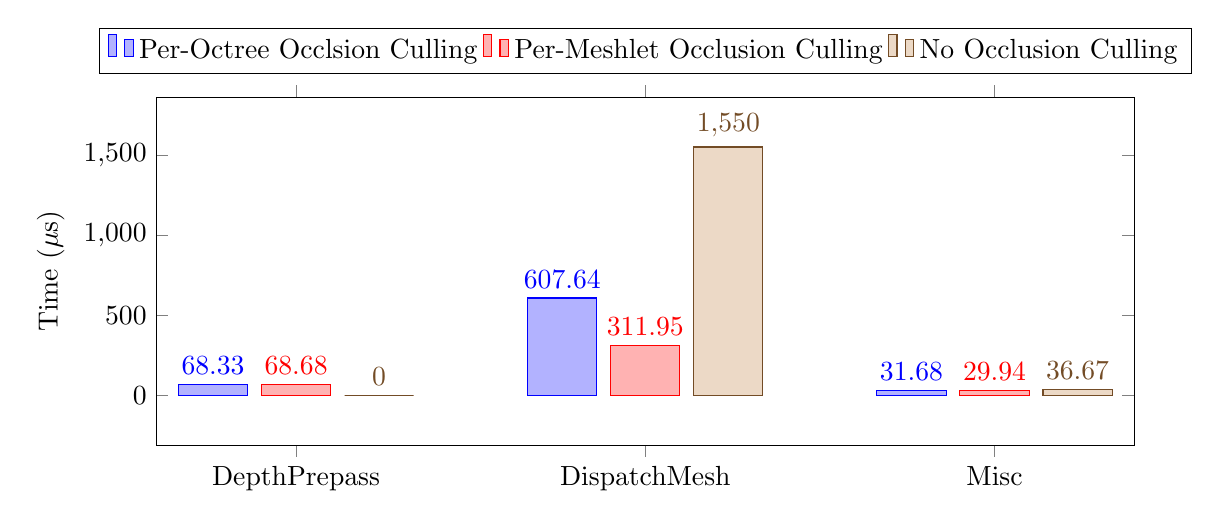
\begin{tikzpicture}
    \begin{axis}[
        height=6cm,
        width=14cm,
        x tick label style={/pgf/number format/1000 sep=},
        ylabel={Time ($\mu$s)},
        legend style={at={(0.5,1.2)}, anchor=north, legend columns=-1},
        symbolic x coords={DepthPrepass, DispatchMesh, Misc},
        xtick=data,
        ybar=0.4,
        bar width=25pt,
        ymin=0,
        nodes near coords,
        enlargelimits=0.2,
    ]
    \addplot+[bar shift=-30pt] coordinates {(DepthPrepass,68.33) (DispatchMesh,607.64) (Misc,31.68)};
    \addplot+[bar shift=0pt] coordinates {(DepthPrepass,68.68) (DispatchMesh,311.95) (Misc,29.9444)};
    \addplot+[bar shift=30pt] coordinates {(DepthPrepass,0) (DispatchMesh,1550.00) (Misc,36.6748)};
    \legend{Per-Octree Occlsion Culling, Per-Meshlet Occlusion Culling, No Occlusion Culling}
    \end{axis}
  \end{tikzpicture}

  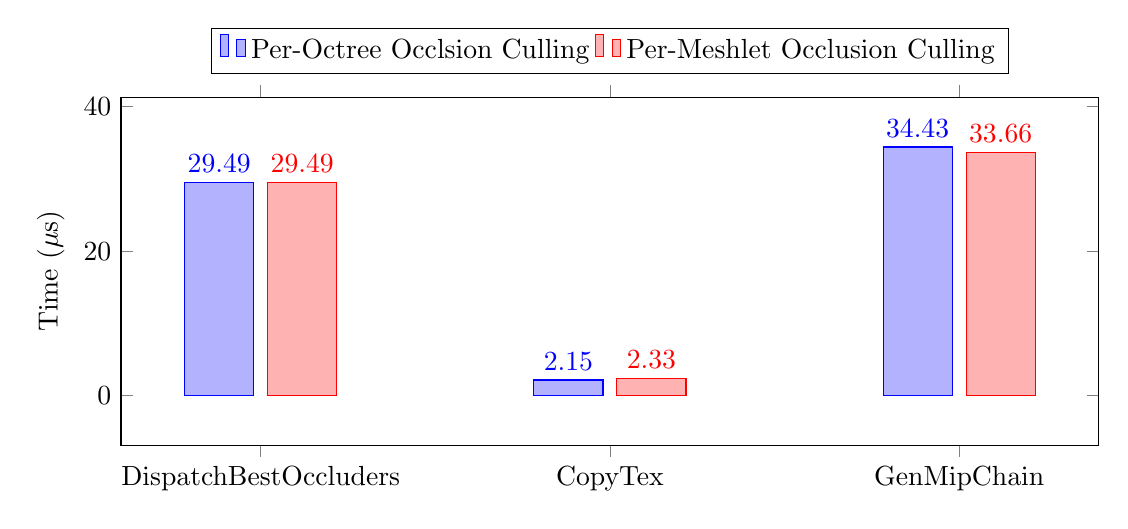
\begin{tikzpicture}
    \begin{axis}[
        height=6cm,
        width=14cm,
        x tick label style={/pgf/number format/1000 sep=},
        ylabel={Time ($\mu$s)},
        legend style={at={(0.5,1.2)}, anchor=north, legend columns=-1},
        symbolic x coords={DispatchBestOccluders, CopyTex, GenMipChain},
        xtick=data,
        ybar=0.4,
        bar width=25pt,
        ymin=0,
        nodes near coords,
        enlargelimits=0.2,
    ]
    \addplot+[bar shift=-15pt] coordinates {(DispatchBestOccluders,29.49) (CopyTex,2.15) (GenMipChain,34.43)};
    \addplot+[bar shift=15pt] coordinates {(DispatchBestOccluders,29.49) (CopyTex,2.33) (GenMipChain,33.66)};
    \legend{Per-Octree Occlsion Culling, Per-Meshlet Occlusion Culling}
    \end{axis}
  \end{tikzpicture}
  \caption{First: The complete time measured on the \ac{GPU}. The \emph{Depth Prepass} is the extra overhead 
  introduced by the \ac{HZB}. The \emph{Dispatch Mesh} is the drawing of the meshes, including the occlusion 
  culling. \emph{Miscellaneous} includes a small amount of \emph{Barriers} used for synchronisation and the 
  rendering of some debug \ac{UI}. It is considered to be more or less static in computation time and is not 
  part of the actual algorithm measured in this experiment. Second: The time measured in the \emph{Depth Prepass}. 
  The \emph{Dispatch Best Occluders} is the drawing to the depth buffer. The \emph{Copy Depth Buffer} computation 
  copies the depth buffers content into the final \ac{HiZ} resource. Finally, \emph{Generate HiZ Pyramid} shows 
  the \ac{HiZ} creation, which is done sequentially.}
  \label{fig:terrain-gpu-times}
\end{figure}

\subsubsection*{Overdraw}

\begin{figure}[!htb]
  \centering
  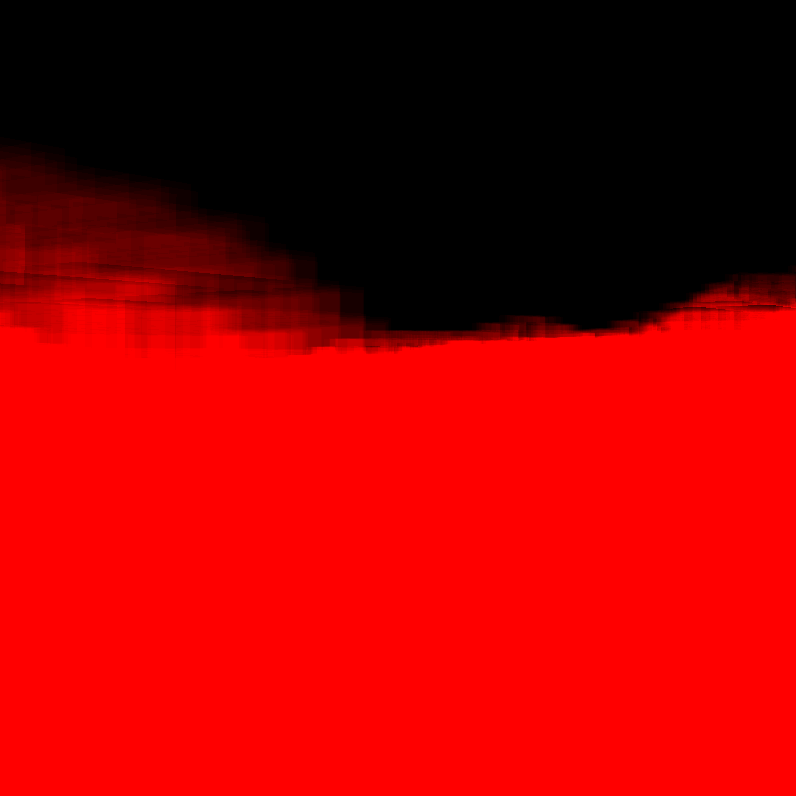
\includegraphics[height=100px]{images/graphics/overdraw-terrain1-nocull.png}
  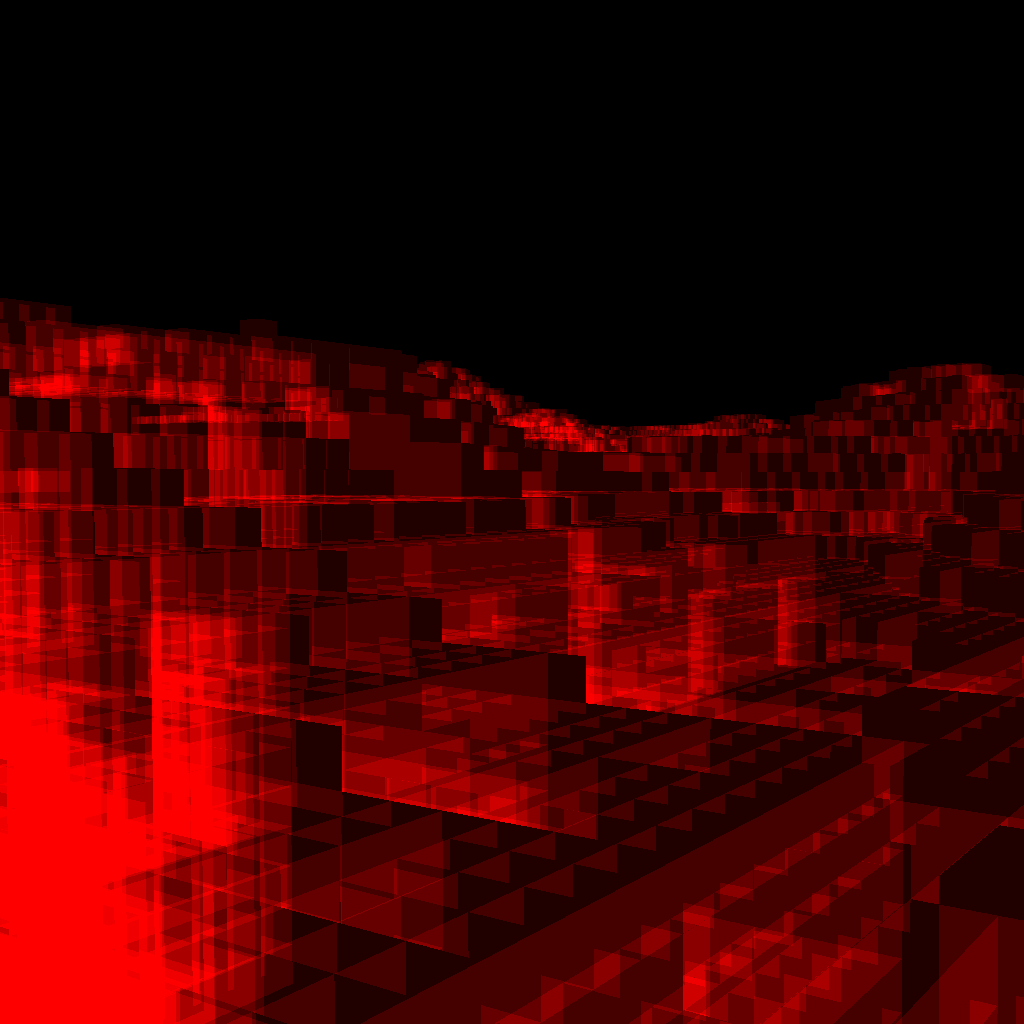
\includegraphics[height=100px]{images/graphics/overdraw-terrain1-pooc.png}
  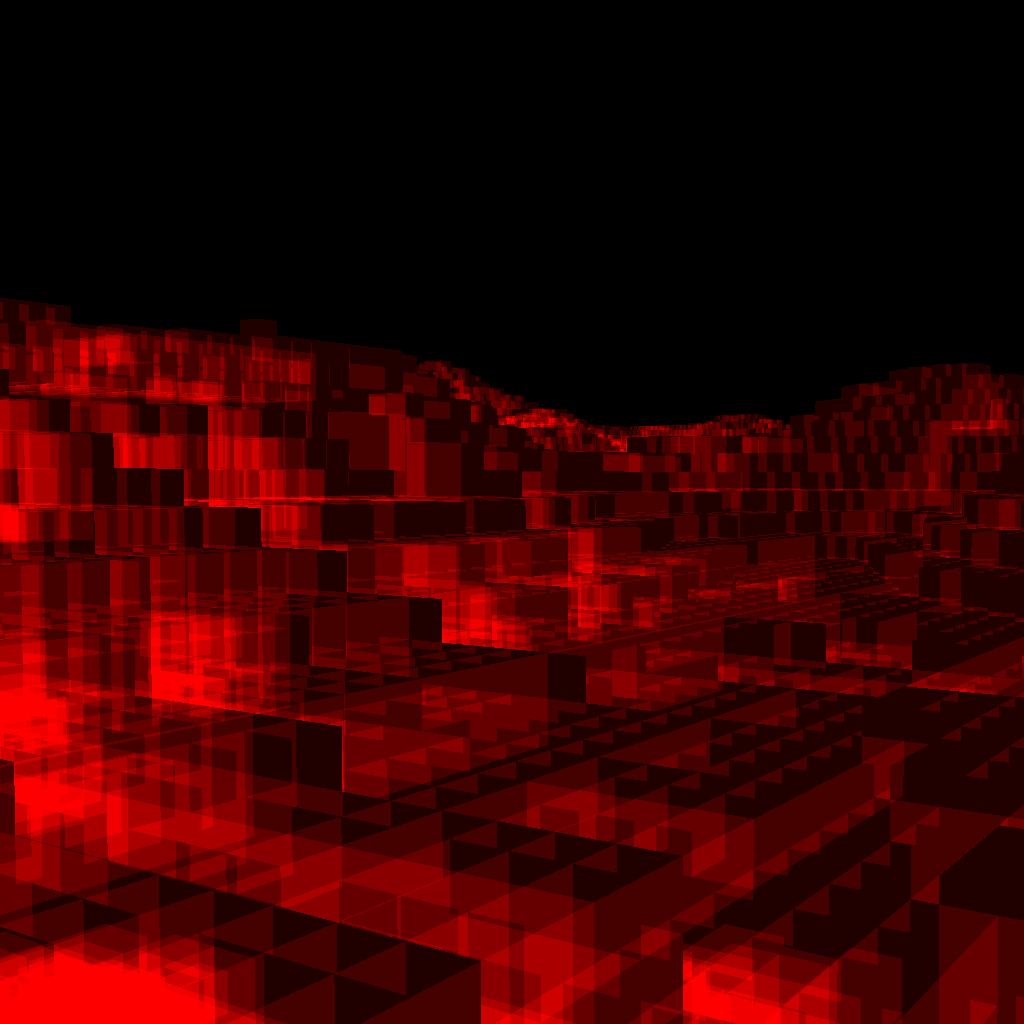
\includegraphics[height=100px]{images/graphics/overdraw-terrain1-pmoc.png}
  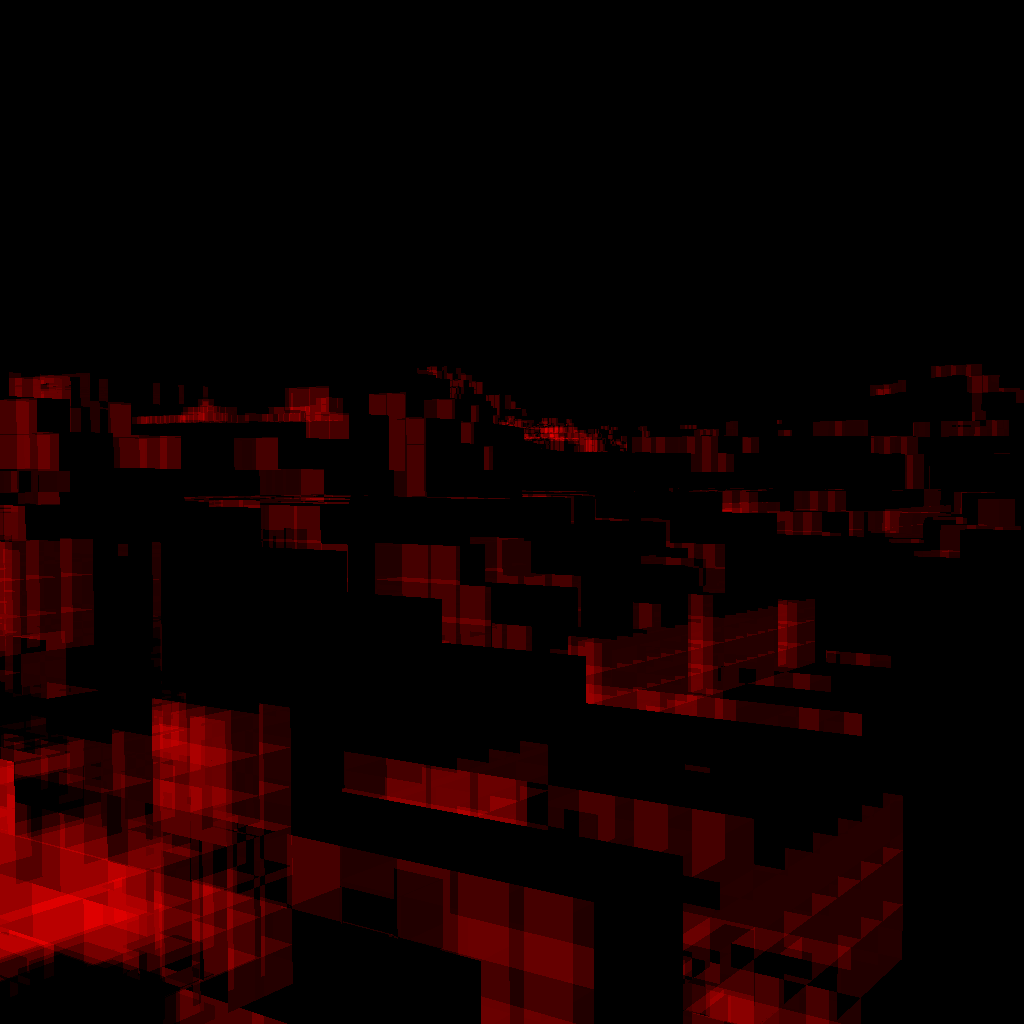
\includegraphics[height=100px]{images/graphics/overdraw-terrain1-diff.png}

  \begin{subfigure}{100px}
    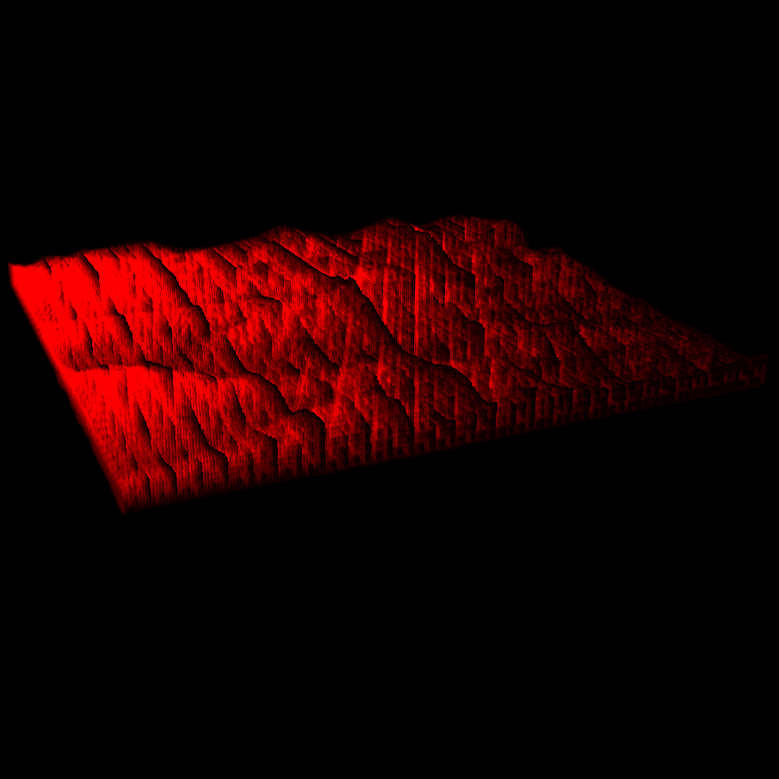
\includegraphics[height=100px]{images/graphics/overdraw-terrain2-nocull.png}
    \caption{}
    \parbox{\linewidth}{\centering\footnotesize No Occlusion\\Culling}
  \end{subfigure}
  \begin{subfigure}{100px}
    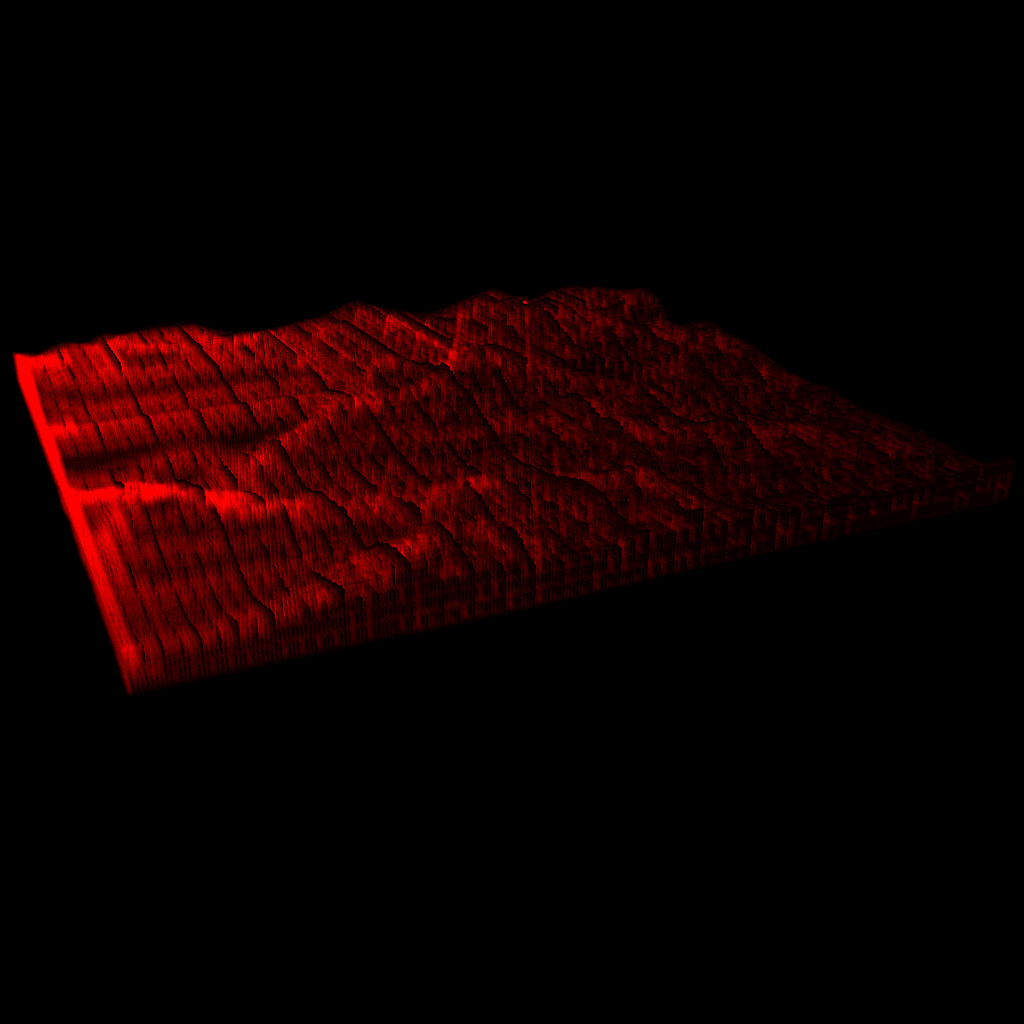
\includegraphics[height=100px]{images/graphics/overdraw-terrain2-pooc.png}
    \caption{}
    \parbox{\linewidth}{\centering\footnotesize Per-Octree Node\\Occlusion Culling}
  \end{subfigure}
  \begin{subfigure}{100px}
    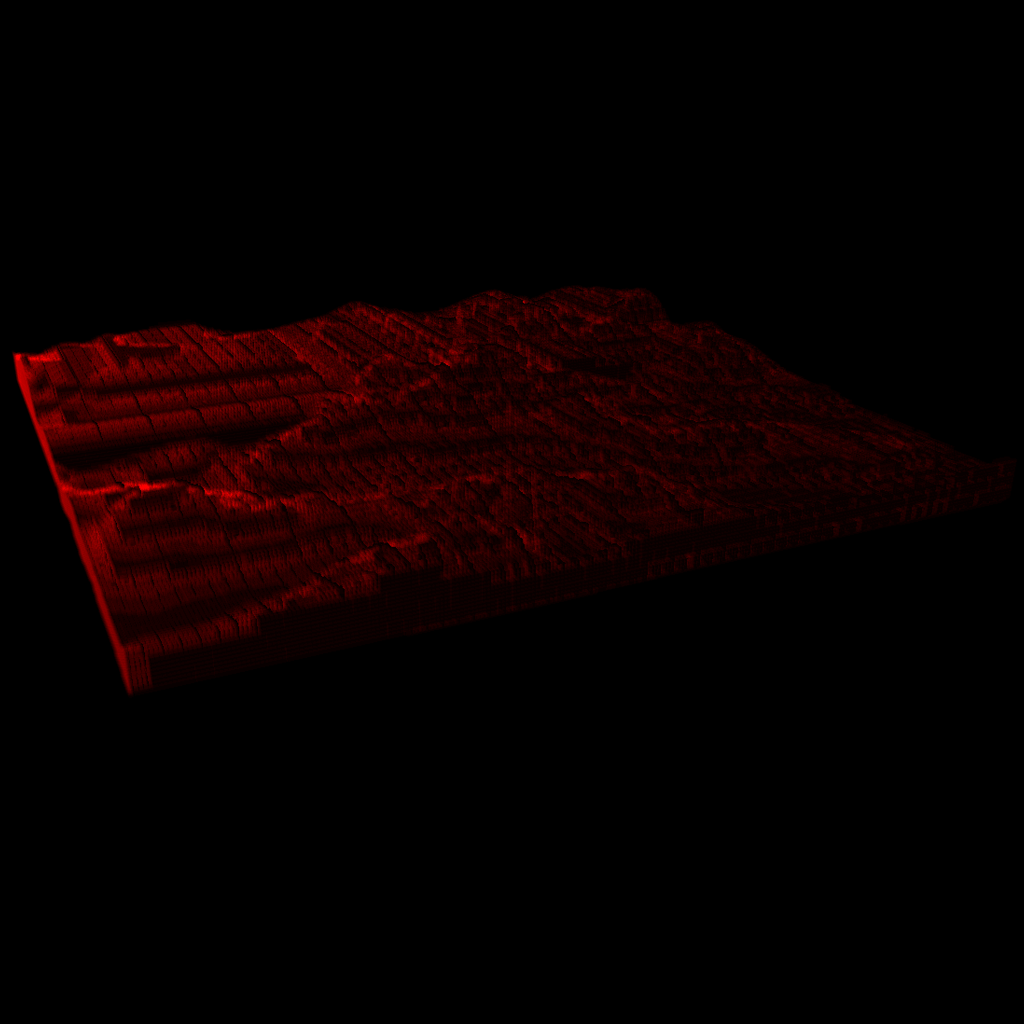
\includegraphics[height=100px]{images/graphics/overdraw-terrain2-pmoc.png}
    \caption{}
    \parbox{\linewidth}{\centering\footnotesize Per-Meshlet\\Occlusion Culling}
  \end{subfigure}
  \begin{subfigure}{100px}
    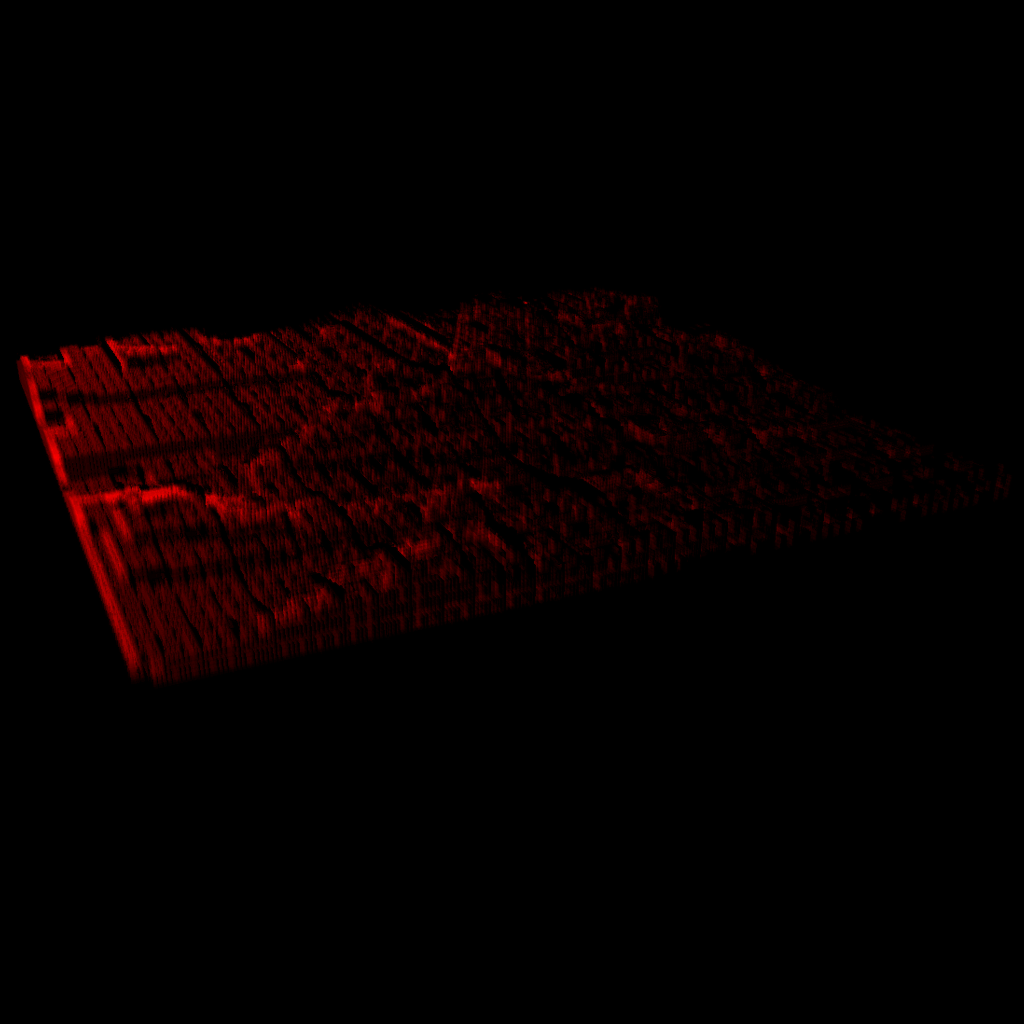
\includegraphics[height=100px]{images/graphics/overdraw-terrain2-diff.png}
    \caption{}
    \parbox{\linewidth}{\centering\footnotesize Difference\\(b) vs. (c)}
  \end{subfigure}

  \caption{Overdraw of the pixels from two different camera angles. 
  The image values are enhanced for better visualization.}
  \label{fig:terrain-overdraw}
\end{figure}


\noindent
As shown in Figure \ref{fig:terrain-overdraw}, the per-octree culling configuration clearly 
featured more overdraw than the comparison configuration. In the first row, it is evident that 
the left lower corner features a lot of overdraw, which was decreased by switching to the 
per-meshlet culling configuration. The maximum draws per pixel were 86 and 45, respectively, in 
favor of the per-meshlet culling. Without culling, the overdraw was 298 draws per pixel.

\clearpage




\subsection*{Hairball}

For low resolutions, the \emph{Hairball} is an inherently complex scene to render. It featuresa lot of 
tiny details, which were assumed to be not sufficient in density to completely fill octree nodes, 
resulting in an unfavorable data layout to test the limits of the occlusion culling algorithm.

\subsubsection*{Culling Results} \label{subsubsec-culling-results-hairball}

Figure \ref{plt:hairball-256-culling-res-voxels} shows the amount of culled voxels and octree nodes 
over the course of the test animation for both occlusion culling configurations. The average culling 
results are marked by the dotted lines in the graph. The hairball model was a particularly interesting 
model because of its fine and thin geometry. It was specifically chosen to provide insights into the 
limitations of the algorithm and to see how it handles models that are not ideal for this use case.\\

\noindent
The results show that the gain in performance wasn't as good for this model as for the other models.
First of all, the number of best occluders was lower than that of the \emph{Terrain} model, even though the 
\emph{Terrain} model had fewer total voxels than the \emph{Hairball} model. This characteristic led to 
a lower probability of octree nodes or meshlets being culled. When looking at the data, the amount of 
voxels being culled on average was $57.8\%$ for \ac{PONOC} and $64.8\%$ for per-meshlet 
occlusion culling, which represented a rather low increase relative to the other models. 

% -------------------------------------- HAIRBALL 256 -------------------------------------

\begin{figure}[!htb]              % Hairball 256 Voxels Test Anim
    \begin{center}
      \begin{tikzpicture}
        \begin{axis}[
            width=\linewidth, % Scale the plot to \linewidth
            height=100px,
            xlabel={Frames},
            ylabel={Visible Voxels},
            grid,
            xmin=0,
            xmax=940,
            ymin=450000,
            ymax=800000,
            legend style={at={(0.5,1.7)}, anchor=north, legend columns=2},
          ]
          \addplot[blue, no marks, solid] table[col sep=comma, x=frame, x expr=\thisrow{frame} * 940 / 940, y=visible_voxels]{./plotdata/hairball_256_voxels.csv};
          \addplot[blue, dotted, no marks, domain=0:940, samples=50] {697549};
          \addplot[red, no marks, solid] table[col sep=comma, x=frame, x expr=\thisrow{frame} * 940 / 1187, y=visible_voxels]{./plotdata/hairball_256_voxels_pmoc.csv};
          \addplot[red, dotted, no marks, domain=0:940, samples=50] {581663};
          \legend{Per-Octree Occlsion Culling, Per-Meshlet Occlusion Culling}
        \end{axis}
      \end{tikzpicture}

      \begin{tikzpicture}
        \begin{axis}[
            width=\linewidth, % Scale the plot to \linewidth
            height=100px,
            xlabel={Frames},
            ylabel={Computed Nodes},
            grid,
            xmin=0,
            xmax=940,
            ymin=15000,
            ymax=25000,
            legend style={at={(0.5,1.7)}, anchor=north, legend columns=2},
          ]
          \addplot[blue, no marks, solid] table[col sep=comma, x=frame, x expr=\thisrow{frame} * 940 / 940, y=visible_nodes]{./plotdata/hairball_256_nodes.csv};
          \addplot[blue, dotted, no marks, domain=0:940, samples=50] {21229};
          \addplot[red, no marks, solid] table[col sep=comma, x=frame, x expr=\thisrow{frame} * 940 / 1187, y=visible_nodes]{./plotdata/hairball_256_nodes_pmoc.csv};
          \addplot[red, dotted, no marks, domain=0:940, samples=50] {18925};
          \legend{Per-Octree Occlsion Culling, Per-Meshlet Occlusion Culling}
        \end{axis}
      \end{tikzpicture}

      \caption{First: The amount of visible voxels over the course of the test animation. 
      Second: The amount of visible octree nodes over the course of the test animation.}
      \label{plt:hairball-256-culling-res-voxels}
    \end{center}
  \end{figure}

% ----------------------------------------------------------------------------------------

\subsubsection*{CPU Performance Results} \label{subsubsec-cpu-performance-results-hairball}

[@TODO: Check: if Render() includes the GPU work, why no difference?]
The \ac{CPU} performance was not significantly diverging and was therefore considered static for 
both configurations. 

\begin{figure}[!htb]              % Hairball CPU times
  \begin{center}
    \begin{tikzpicture}
      \begin{axis}[
          width=\linewidth,
          height=100px,
          xlabel={Frames},
          ylabel={Update Time (s)},
          grid,
          xmin=0,
          xmax=940,
          ymin=0,
          ymax=0.00005,
          legend style={at={(0.5,1.7)}, anchor=north, legend columns=2},
        ]
        \addplot[brown!60, no marks, solid] table[col sep=comma, x=frame, x expr=\thisrow{frame} * 940 / 1301, y=time]{./plotdata/cpu/hairball_256_updateTime_nocull.csv};
        \addplot[blue, no marks, solid] table[col sep=comma, x=frame, x expr=\thisrow{frame} * 940 / 1421, y=time]{./plotdata/cpu/hairball_256_updateTime_pooc.csv};
        \addplot[red, no marks, solid] table[col sep=comma, x=frame, x expr=\thisrow{frame} * 940 / 1446, y=time]{./plotdata/cpu/hairball_256_updateTime.csv};
        \legend{No Occlusion Culling, Per-Octree Occlsion Culling, Per-Meshlet Occlusion Culling}
      \end{axis}
    \end{tikzpicture}
    \begin{tikzpicture}
      \begin{axis}[
          width=\linewidth,
          height=100px,
          xlabel={Frames},
          ylabel={Render Time (s)},
          grid,
          xmin=0,
          xmax=940,
          ymin=0,
          ymax=0.00025,
          legend style={at={(0.5,1.7)}, anchor=north, legend columns=2},
        ]
        \addplot[brown!60, no marks, solid] table[col sep=comma, x=frame, x expr=\thisrow{frame} * 940 / 1301, y=time]{./plotdata/cpu/hairball_256_renderTime_nocull.csv};
        \addplot[blue, no marks, solid] table[col sep=comma, x=frame, x expr=\thisrow{frame} * 940 / 1421, y=time]{./plotdata/cpu/hairball_256_renderTime_pooc.csv};
        \addplot[red, no marks, solid] table[col sep=comma, x=frame, x expr=\thisrow{frame} * 940 / 1446, y=time]{./plotdata/cpu/hairball_256_renderTime.csv};
        \legend{No Occlusion Culling, Per-Octree Occlsion Culling, Per-Meshlet Occlusion Culling}
      \end{axis}
    \end{tikzpicture}
    \caption{Overview of the render times over the course of the test animation. The upper graph shows the time 
    each frame took to execute the \emph{Update()} function on the \ac{CPU}. The lower graph shows the time each 
    frame took to execute the function \emph{Render()} on the \ac{CPU}. This includes the completion of the 
    \ac{GPU} computations.}
    \label{plt:hairball-256-culling-cpu-time}
  \end{center}
\end{figure}

\subsubsection*{GPU Performance Results} \label{subsubsec-gpu-performance-results-hairball}

Figure \ref{fig:hairball-gpu-times} shows the difference in \ac{GPU} timing, which was in favor of the 
\ac{PMOC}. Although the per-meshlet culling configuration still accelerated the \ac{GPU} 
operations, the differences got smaller compared to the other models, yielding only a $14.9\%$ decrease in 
computation time on average. The depth prepass diverged by only 0.75 microseconds in favor of the per-meshlet 
occlusion culling when comparing the average values.  

\begin{figure}[!htb]
  \centering
  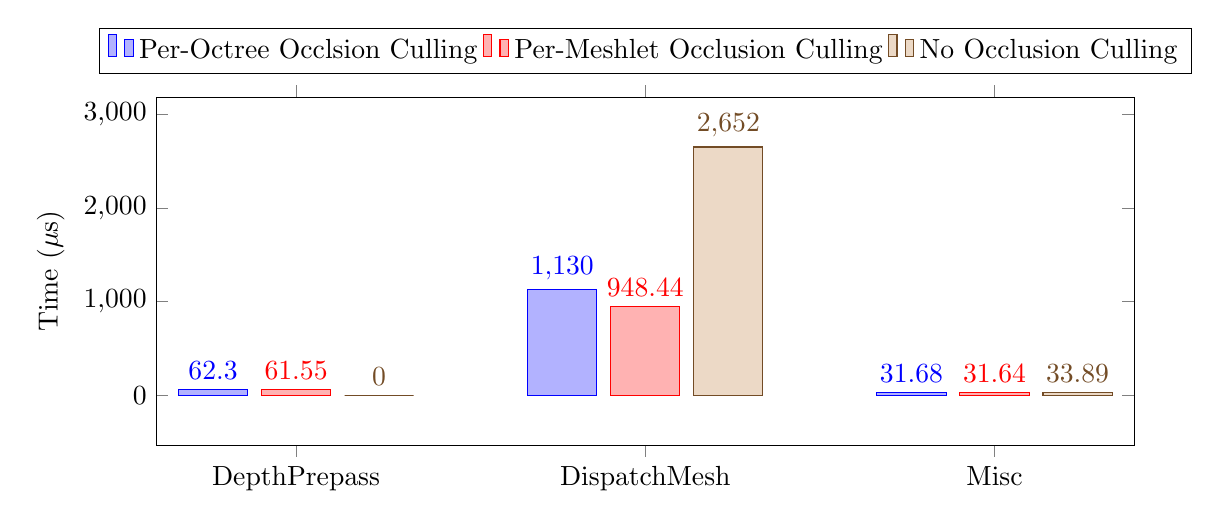
\begin{tikzpicture}
    \begin{axis}[
        height=6cm,
        width=14cm,
        x tick label style={/pgf/number format/1000 sep=},
        ylabel={Time ($\mu$s)},
        legend style={at={(0.5,1.2)}, anchor=north, legend columns=-1},
        symbolic x coords={DepthPrepass, DispatchMesh, Misc},
        xtick=data,
        ybar=0.4,
        bar width=25pt,
        ymin=0,
        nodes near coords,
        enlargelimits=0.2,
    ]
    \addplot+[bar shift=-30pt] coordinates {(DepthPrepass,62.30) (DispatchMesh,1130.00) (Misc,31.68)};
    \addplot+[bar shift=0pt] coordinates {(DepthPrepass,61.55) (DispatchMesh,948.44) (Misc,31.6354)};
    \addplot+[bar shift=30pt] coordinates {(DepthPrepass,0) (DispatchMesh,2652.00) (Misc,33.8856)};
    \legend{Per-Octree Occlsion Culling, Per-Meshlet Occlusion Culling, No Occlusion Culling}
    \end{axis}
  \end{tikzpicture}

  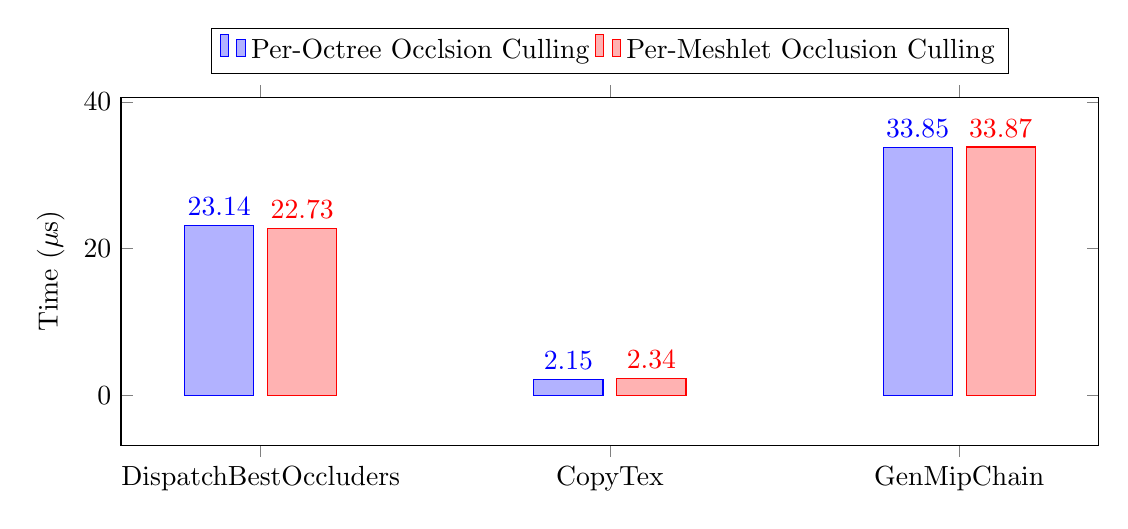
\begin{tikzpicture}
    \begin{axis}[
        height=6cm,
        width=14cm,
        x tick label style={/pgf/number format/1000 sep=},
        ylabel={Time ($\mu$s)},
        legend style={at={(0.5,1.2)}, anchor=north, legend columns=-1},
        symbolic x coords={DispatchBestOccluders, CopyTex, GenMipChain},
        xtick=data,
        ybar=0.4,
        bar width=25pt,
        ymin=0,
        nodes near coords,
        enlargelimits=0.2,
    ]
    \addplot+[bar shift=-15pt] coordinates {(DispatchBestOccluders,23.14) (CopyTex,2.15) (GenMipChain,33.85)};
    \addplot+[bar shift=15pt] coordinates {(DispatchBestOccluders,22.73) (CopyTex,2.34) (GenMipChain,33.87)};
    \legend{Per-Octree Occlsion Culling, Per-Meshlet Occlusion Culling}
    \end{axis}
  \end{tikzpicture}
  \caption{First: The complete time measured on the \ac{GPU}. The \emph{Depth Prepass} is the extra overhead 
  introduced by the \ac{HZB}. The \emph{Dispatch Mesh} is the drawing of the meshes, including the occlusion 
  culling. \emph{Miscellaneous} includes a small amount of \emph{Barriers} used for synchronisation and the 
  rendering of some debug \ac{UI}. It is considered to be more or less static in computation time and is not 
  part of the actual algorithm measured in this experiment. Second: The time measured in the \emph{Depth Prepass}. 
  The \emph{Dispatch Best Occluders} is the drawing to the depth buffer. The \emph{Copy Depth Buffer} computation 
  copies the depth buffers content into the final \ac{HiZ} resource. Finally, \emph{Generate HiZ Pyramid} shows 
  the \ac{HiZ} creation, which is done sequentially.}
  \label{fig:hairball-gpu-times}
\end{figure}

\noindent
The data clearly indicates that the \emph{Hairball} model wasn't using the culling algorithm as efficiently as 
the other models did. From this, it is possible to derive how the algorithm should ideally be applied and in 
which use case the overhead is greater than the time saving.

\subsubsection*{Overdraw}

\begin{figure}[!htb]
  \centering  
  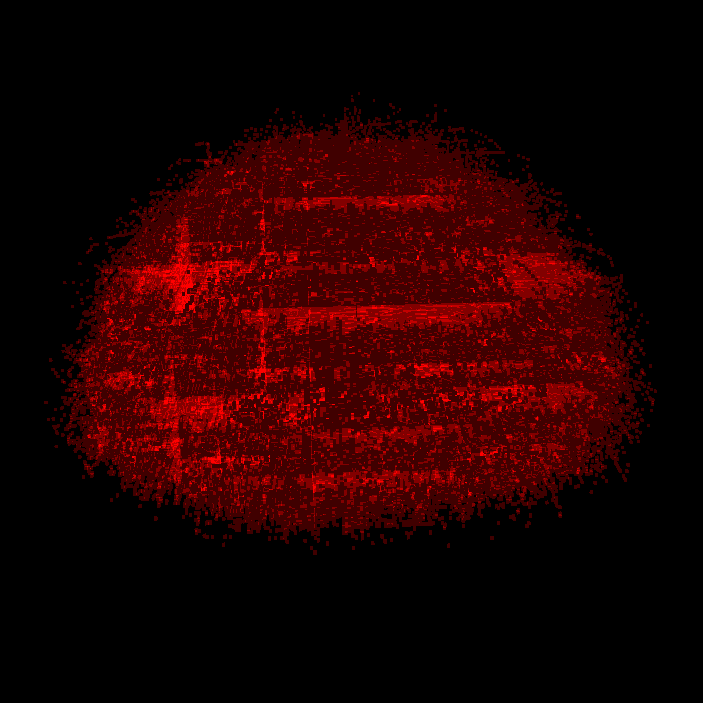
\includegraphics[height=100px]{images/graphics/overdraw-hairball1-nocull.png}
  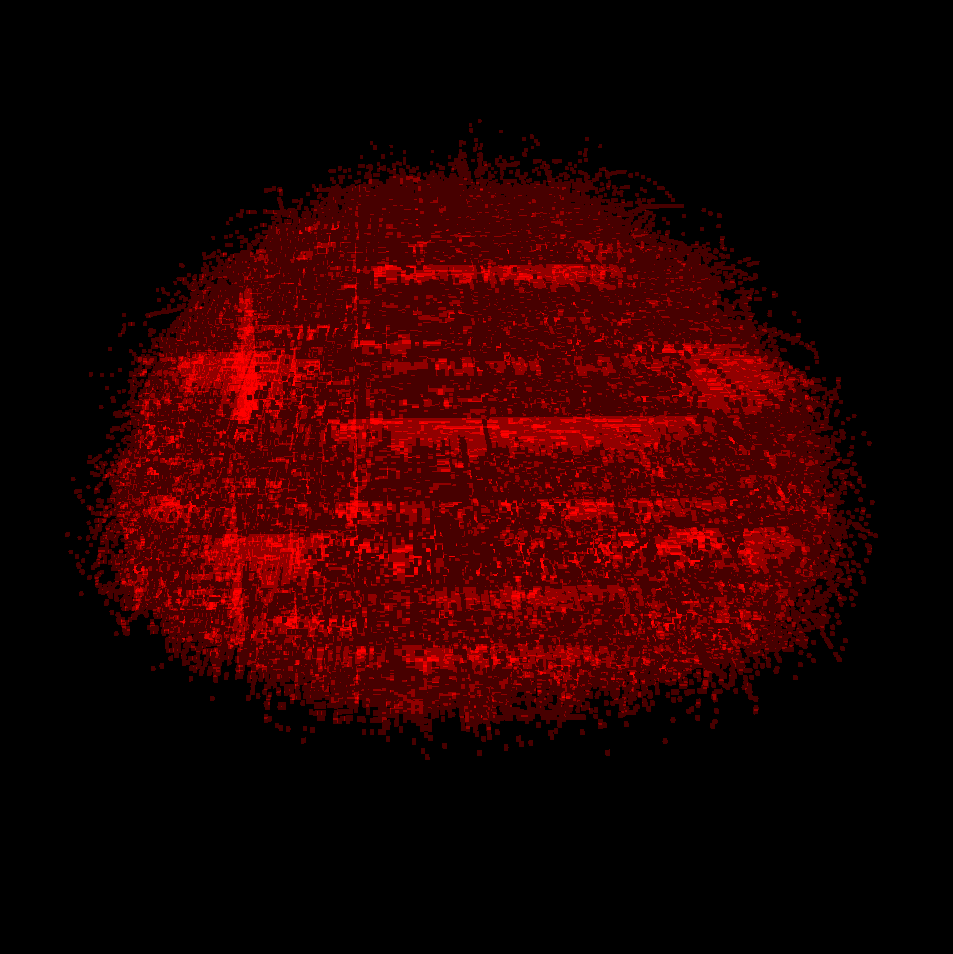
\includegraphics[height=100px]{images/graphics/overdraw-hairball1-pooc.png}
  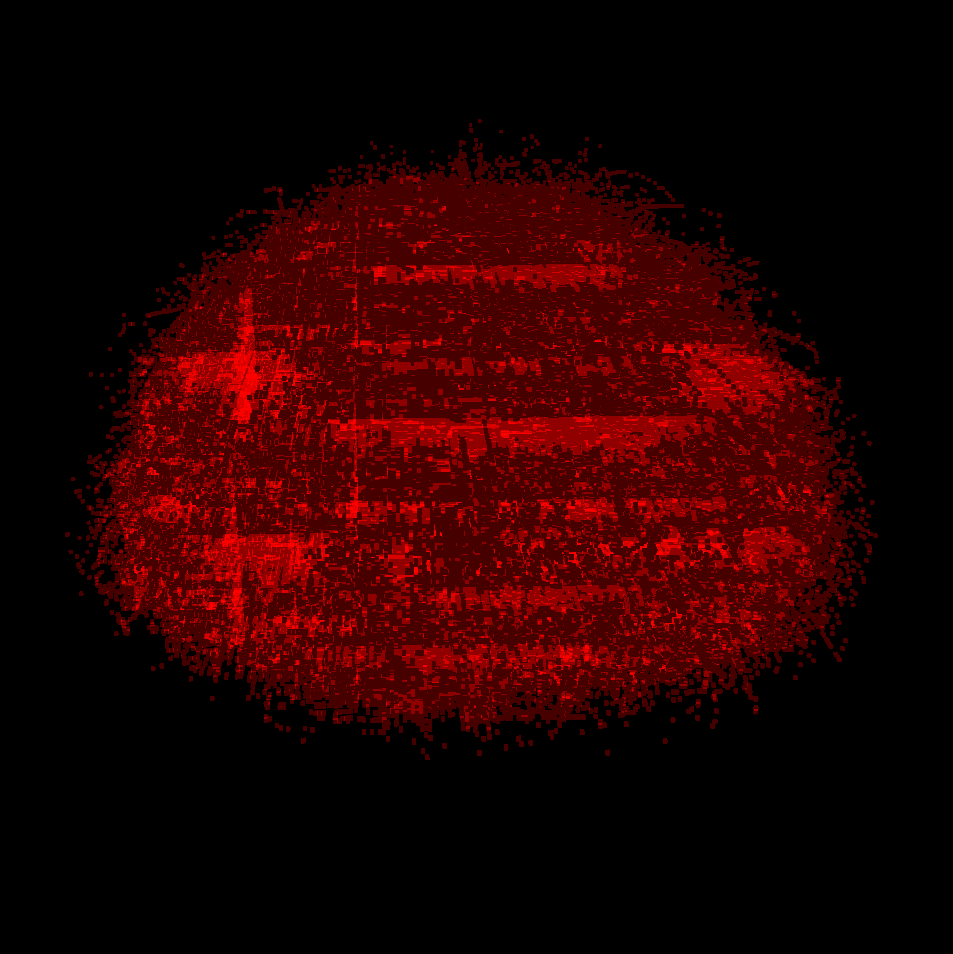
\includegraphics[height=100px]{images/graphics/overdraw-hairball1-pmoc.png}
  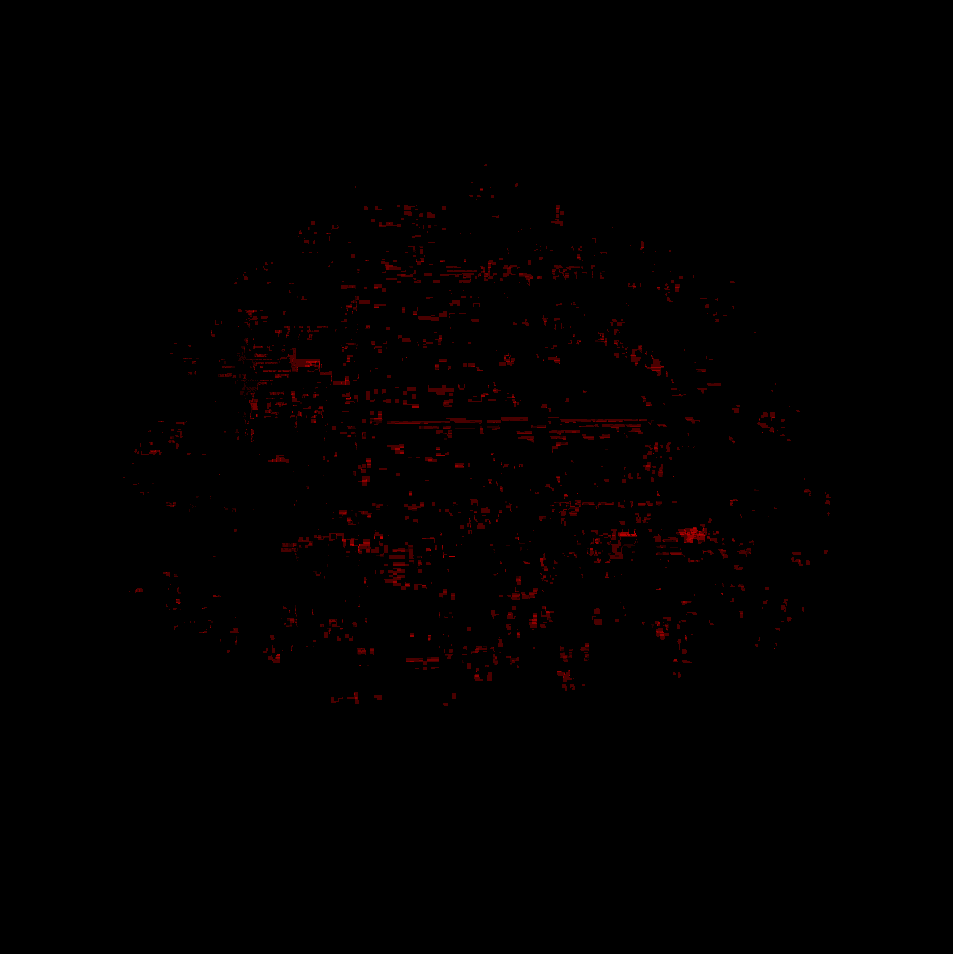
\includegraphics[height=100px]{images/graphics/overdraw-hairball1-diff.png}

  \begin{subfigure}{100px}
    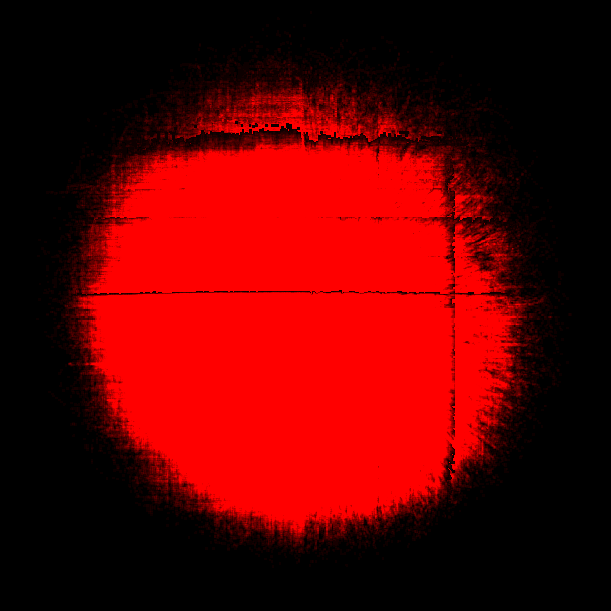
\includegraphics[height=100px]{images/graphics/overdraw-hairball2-nocull.png}
    \caption{}
    \parbox{\linewidth}{\centering\footnotesize No Occlusion\\Culling}
  \end{subfigure}
  \begin{subfigure}{100px}
    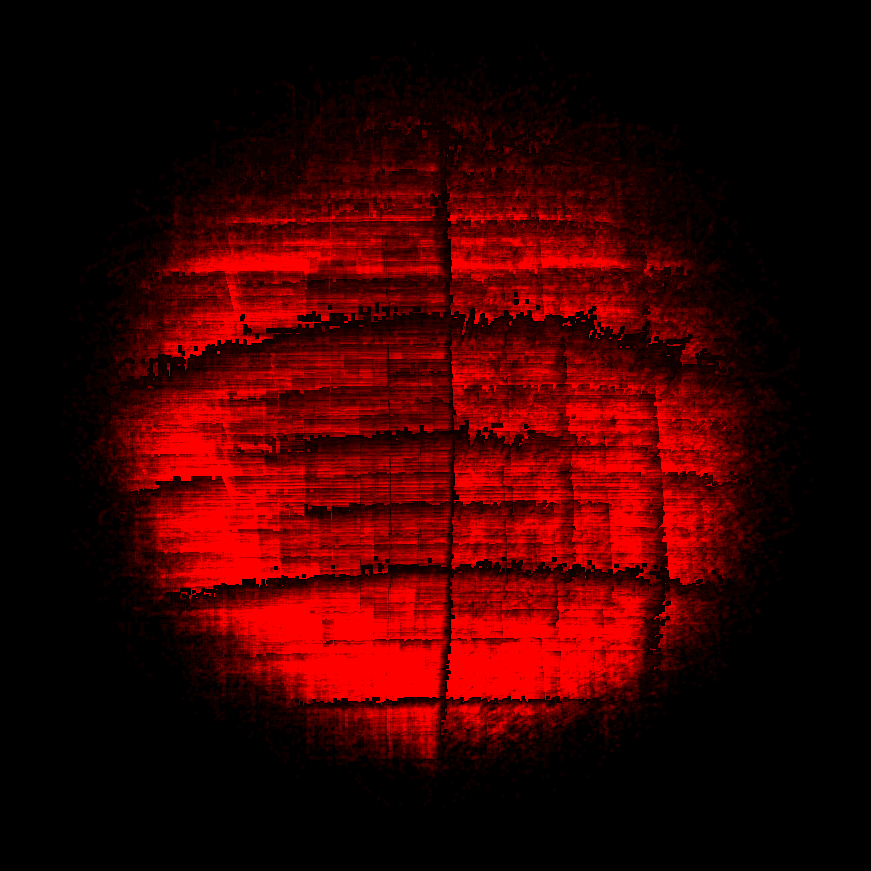
\includegraphics[height=100px]{images/graphics/overdraw-hairball2-pooc.png}
    \caption{}
    \parbox{\linewidth}{\centering\footnotesize Per-Octree Node\\Occlusion Culling}
  \end{subfigure}
  \begin{subfigure}{100px}
    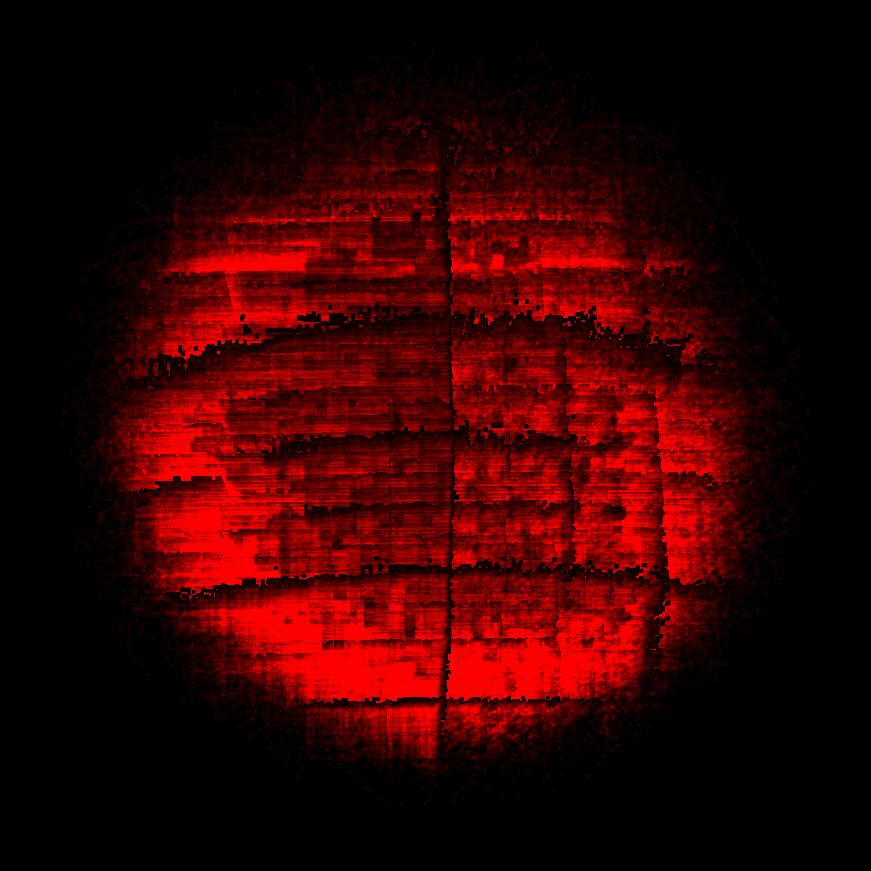
\includegraphics[height=100px]{images/graphics/overdraw-hairball2-pmoc.png}
    \caption{}
    \parbox{\linewidth}{\centering\footnotesize Per-Meshlet\\Occlusion Culling}
  \end{subfigure}
  \begin{subfigure}{100px}
    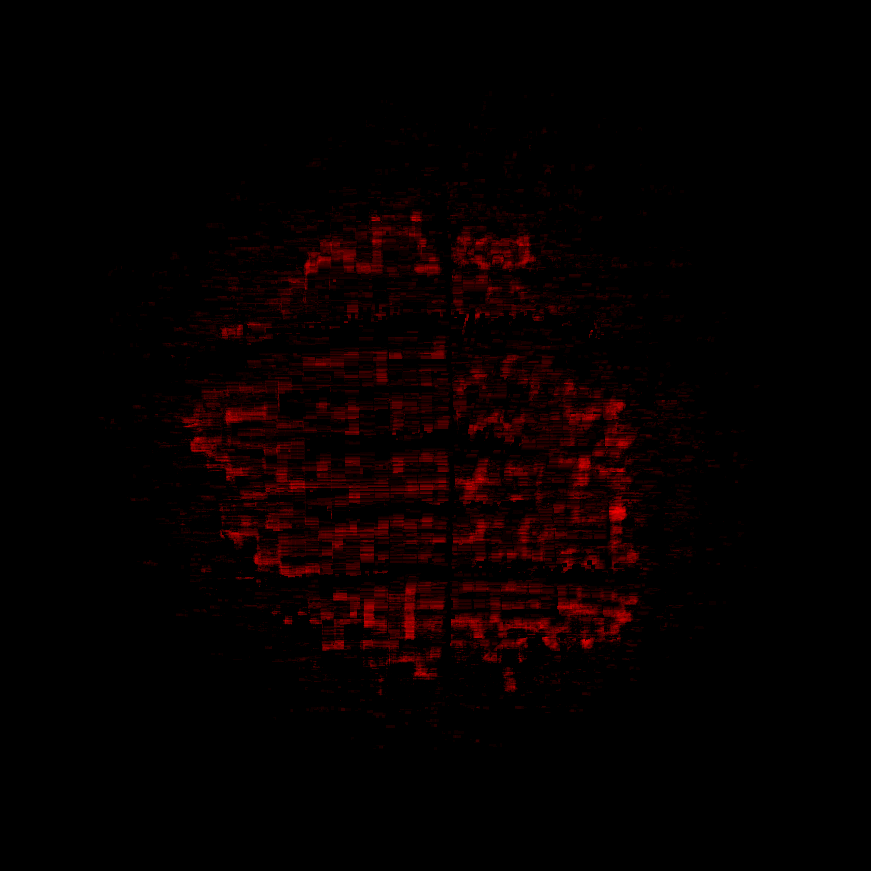
\includegraphics[height=100px]{images/graphics/overdraw-hairball2-diff.png}
    \caption{}
    \parbox{\linewidth}{\centering\footnotesize Difference\\(b) vs. (c)}
  \end{subfigure}

  \caption{Overdraw of the pixels from two different camera angles. 
  The image values are enhanced for better visualization.}
  \label{fig:hairball-overdraw}
\end{figure}

\noindent
Figure \ref{fig:hairball-overdraw} shows that the overdraw was similar for both configurations, 
but still in favor of \ac{PMOC}. The last column featuring the difference 
values between both configurations shows this particularly well. There is only a small difference 
between both measurements, which is also reflected in the maximum amount of overdraw. The 
per-octree node culling resulted in a maximum of 54 draws to one pixel, and the per-meshlet 
culling configuration resulted in a maximum of 51 draws. Without occlusion culling, the overdraw 
reached its maximum at 117 draws to one pixel. 

Again, the top view resulted in more 
overdraw than the front view.

\clearpage




\section*{Measurment Overview}

Now that each model has been analyzed individually, the data is cross-compared over all models to 
discuss the overall results the measurements provided. Table \ref{tbl:culling-result-overview} shows 
an overview of all models and some of the most interesting data points. 
  
\begin{table}[!htb]
  \begin{tabular}{|lccccc|}
    \hline
    \multicolumn{1}{|l|}{}                          & \multicolumn{1}{|c|}{\textbf{Stanford Lucy}}  & \multicolumn{1}{c|}{\textbf{Stanford Bunny}}  & \multicolumn{1}{c|}{\textbf{Torus}}   & \multicolumn{1}{c|}{\textbf{Terrain}}     & \multicolumn{1}{c|}{\textbf{Hairball}}    \\ \hline
    \multicolumn{1}{|l|}{Best Occluder Count}       & \multicolumn{1}{c|}{1600}                     & \multicolumn{1}{c|}{8256}                     & \multicolumn{1}{c|}{7168}             & \multicolumn{1}{c|}{6976}                 & \multicolumn{1}{c|}{5056}                 \\ 
    \multicolumn{1}{|l|}{Total Voxel Count}         & \multicolumn{1}{c|}{331,254}                  & \multicolumn{1}{c|}{3,379,738}                & \multicolumn{1}{c|}{2,311,006}        & \multicolumn{1}{c|}{953,362}              & \multicolumn{1}{c|}{1,652,435}            \\
    \multicolumn{1}{|l|}{Total Octree Nodes}        & \multicolumn{1}{c|}{6,830}                    & \multicolumn{1}{c|}{57,481}                   & \multicolumn{1}{c|}{39,794}           & \multicolumn{1}{c|}{18,465}               & \multicolumn{1}{c|}{39,591}               \\
    \multicolumn{1}{|l|}{Avg. Node Population}      & \multicolumn{1}{c|}{\textbf{48.5 \%}}         & \multicolumn{1}{c|}{\textbf{91.9 \%}}         & \multicolumn{1}{c|}{\textbf{90.7 \%}} & \multicolumn{1}{c|}{\textbf{80.7 \%}}     & \multicolumn{1}{c|}{\textbf{65.2 \%}}     \\ \hline
    \multicolumn{6}{|c|}{\textbf{Scene Resolution: $256^3$ - Per-Octree Occlusion Culling}}                                                                                                                                                                                         \\ \hline
    \multicolumn{1}{|l|}{Avg. Visible Voxels}       & \multicolumn{1}{c|}{140,842}                  & \multicolumn{1}{c|}{385,210}                  & \multicolumn{1}{c|}{359,313}          & \multicolumn{1}{c|}{396,228}              & \multicolumn{1}{c|}{697,549}              \\
    \multicolumn{1}{|l|}{Avg. Culled Voxels}        & \multicolumn{1}{c|}{190,412}                  & \multicolumn{1}{c|}{2,994,528}                & \multicolumn{1}{c|}{1,951,693}        & \multicolumn{1}{c|}{557,134}              & \multicolumn{1}{c|}{954,886}              \\
    \multicolumn{1}{|l|}{Avg. Culled Voxel Ratio}   & \multicolumn{1}{c|}{\textbf{57.5 \%}}         & \multicolumn{1}{c|}{\textbf{88.6 \%}}         & \multicolumn{1}{c|}{\textbf{84.5 \%}} & \multicolumn{1}{c|}{\textbf{58.4 \%}}     & \multicolumn{1}{c|}{\textbf{57.8 \%}}     \\ \hline
    \multicolumn{1}{|l|}{Avg. Visible Nodes}        & \multicolumn{1}{c|}{3,460}                    & \multicolumn{1}{c|}{8,519}                    & \multicolumn{1}{c|}{7,712}            & \multicolumn{1}{c|}{8,207}                & \multicolumn{1}{c|}{21,229}               \\
    \multicolumn{1}{|l|}{Avg. Culled Nodes}         & \multicolumn{1}{c|}{3,370}                    & \multicolumn{1}{c|}{48,962}                   & \multicolumn{1}{c|}{32,082}           & \multicolumn{1}{c|}{10,258}               & \multicolumn{1}{c|}{18,362}               \\
    \multicolumn{1}{|l|}{Avg. Culled Node Ratio}    & \multicolumn{1}{c|}{\textbf{49.3 \%}}         & \multicolumn{1}{c|}{\textbf{85.2 \%}}         & \multicolumn{1}{c|}{\textbf{80.6 \%}} & \multicolumn{1}{c|}{\textbf{55.6 \%}}     & \multicolumn{1}{c|}{\textbf{46.4 \%}}     \\ \hline
    \multicolumn{6}{|c|}{\textbf{Scene Resolution: $256^3$ - Per-Meshlet Occlusion Culling}}                                                                                                                                                                                        \\ \hline
    \multicolumn{1}{|l|}{Avg. Visible Voxels}       & \multicolumn{1}{c|}{84,082}                   & \multicolumn{1}{c|}{180,266}                  & \multicolumn{1}{c|}{170,772}          & \multicolumn{1}{c|}{180,440}              & \multicolumn{1}{c|}{581,663}              \\
    \multicolumn{1}{|l|}{Avg. Culled Voxels}        & \multicolumn{1}{c|}{247,226}                  & \multicolumn{1}{c|}{3,199,472}                & \multicolumn{1}{c|}{2,140,234}        & \multicolumn{1}{c|}{772,922}              & \multicolumn{1}{c|}{1,070,722}            \\
    \multicolumn{1}{|l|}{Avg. Culled Voxel Ratio}   & \multicolumn{1}{c|}{\textbf{74.6 \%}}         & \multicolumn{1}{c|}{\textbf{94.7 \%}}         & \multicolumn{1}{c|}{\textbf{92.6 \%}} & \multicolumn{1}{c|}{\textbf{81.1 \%}}     & \multicolumn{1}{c|}{\textbf{64.8 \%}}     \\ \hline
    \multicolumn{1}{|l|}{Avg. Visible Nodes}        & \multicolumn{1}{c|}{2,483}                    & \multicolumn{1}{c|}{5,415}                    & \multicolumn{1}{c|}{4,768}            & \multicolumn{1}{c|}{3,832}                & \multicolumn{1}{c|}{18,925}               \\
    \multicolumn{1}{|l|}{Avg. Culled Nodes}         & \multicolumn{1}{c|}{4,347}                    & \multicolumn{1}{c|}{52,066}                   & \multicolumn{1}{c|}{35,026}           & \multicolumn{1}{c|}{14,633}               & \multicolumn{1}{c|}{20,666}               \\
    \multicolumn{1}{|l|}{Avg. Culled Node Ratio}    & \multicolumn{1}{c|}{\textbf{63.6 \%}}         & \multicolumn{1}{c|}{\textbf{90.6 \%}}         & \multicolumn{1}{c|}{\textbf{88.0 \%}} & \multicolumn{1}{c|}{\textbf{79.2 \%}}     & \multicolumn{1}{c|}{\textbf{52.2 \%}}     \\ \hline
    
  \end{tabular}
  \caption{An overview comparing the most significant measures for all models. 
  The table shows results for the \ac{PONOC} configuration and below for the 
  \ac{PMOC} configuration.}
  \label{tbl:culling-result-overview}
\end{table}
  
\noindent
The table shows the average culling data for all models. The row \emph{Average Node Population} is 
particularly interesting as it shows how the culling results related to the degree to which the octree 
nodes were filled. The higher this value, the more the octree nodes were filled on average. A high 
average fill indicates the existence of a lot of best occluders relative the amount of voxels and 
octree nodes present in the scene. This measure strongly correlates with the average ratio of culled 
coxels and octree nodes. \\

\noindent
The table also shows the same aspects for the \ac{PMOC} configuration. It shows that the 
occlusion culling algorithm was able to cull a greater amount of voxels when using the per-meshlet culling 
configuration. Additionally, across all models, a higher amount of best occluders consequently resulted in a 
higher culling ratio, and the average node population correlated with the average voxel culling ratio.

\begin{figure}    % GPU time overview
  \begin{center}
    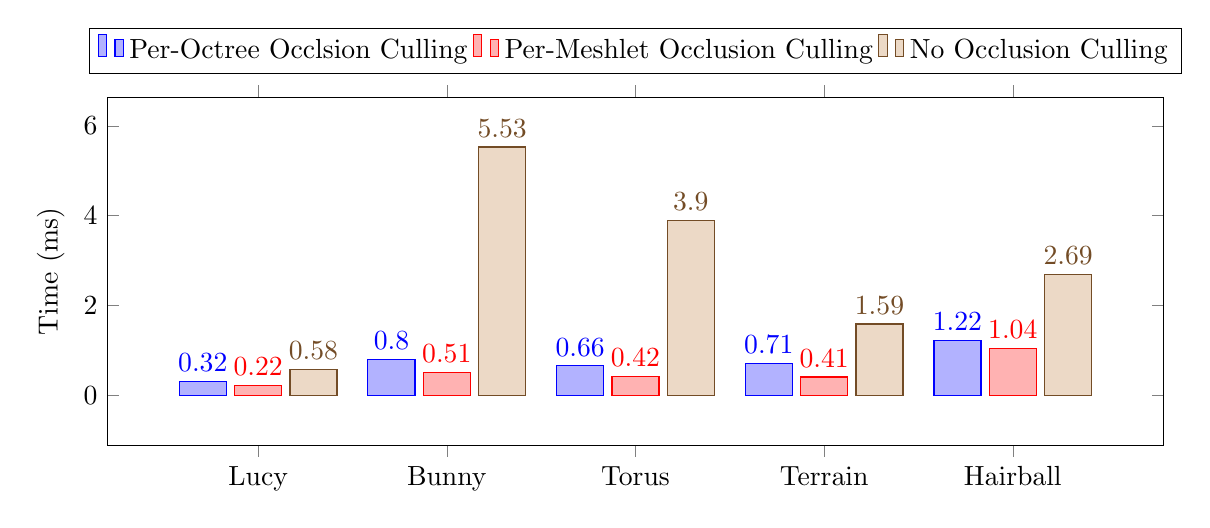
\begin{tikzpicture}
      \begin{axis}[
          height=6cm,
          width=15cm,
          x tick label style={/pgf/number format/1000 sep=},
          ylabel={Time (ms)},
          legend style={at={(0.5,1.2)}, anchor=north, legend columns=-1},
          symbolic x coords={Lucy, Bunny, Torus, Terrain, Hairball},
          xtick=data,
          ybar=0.4,
          bar width=17pt,
          ymin=0,
          nodes near coords,
          enlargelimits=0.2,
      ]
      \addplot+[bar shift=-20pt] coordinates {(Lucy,0.32) (Bunny,0.80) (Torus,0.66) (Terrain,0.71) (Hairball,1.22)};
      \addplot+[bar shift=0pt] coordinates {(Lucy,0.22) (Bunny,0.51) (Torus,0.42) (Terrain,0.41) (Hairball,1.04)};
      \addplot+[bar shift=20pt] coordinates {(Lucy,0.58) (Bunny,5.53) (Torus,3.90) (Terrain,1.59) (Hairball,2.69)};
      \legend{Per-Octree Occlsion Culling, Per-Meshlet Occlusion Culling, No Occlusion Culling}
      \end{axis}
    \end{tikzpicture}
  \end{center}
  \caption{An overview of the average \ac{GPU} timings for all tested models.}
  \label{fig:gpu-performance-overview}
\end{figure}

\noindent
The measurements show that the culling significantly benefitted the \ac{GPU} performance throughout all 
models. Figure \ref{fig:gpu-performance-overview} shows an overview of all models comparing the time spent 
on the \ac{GPU} between both tested configurations. The \ac{CPU} performance did not show any significant 
differences that could reliably be traced back to the tested approaches. Small differences were usually in the 
order of about 1-10 microseconds and could not be reliably attributed to either of the two culling 
configurations. \\


\noindent
The individual overdraw measurements indicate that the amount of overdraw significantly varies with the 
change of the camera angle. It is evident that the overdraw could be reduced best using models with high 
volumes and avoiding small and thin details. In general, the per-meshlet culling approach was able to 
achieve better results in terms of overdraw, although it was highly dependent on camera angle and dense 
best occluder coverage. Usually, outer edges of models with curved surfaces could not be covered very well 
because of the lack of best occluders. \\



[@TODO: Add throughput data]
[@TODO: Where do I write about the scaling of computation times with screen res / voxel count / ...?]